\documentclass{article}

% Language setting
% Replace `english' with e.g. `spanish' to change the document language
\usepackage[ngerman]{babel}
% Set page size and margins
% Replace `letterpaper' with`a4paper' for UK/EU standard size
\usepackage[letterpaper,top=2cm,bottom=2cm,left=3cm,right=3cm,marginparwidth=1.75cm]{geometry}
% Useful packages
\usepackage{amsmath}
\usepackage{graphicx}
\usepackage[colorlinks=true, allcolors=blue]{hyperref}

\usepackage[utf8]{inputenc}
\usepackage{xcolor}
\usepackage{graphicx}
\usepackage[style=numeric, backend=biber]{biblatex}
\usepackage{fvextra}
\usepackage{csquotes}
\usepackage{svg}
\usepackage{amsmath}
\usepackage{datetime}
\usepackage{hyperref}
\usepackage[font={small,it}]{caption}
\usepackage{acronym}
\usepackage{listings}
\usepackage[T1]{fontenc}
\usepackage{subfig}

\usepackage{CJKutf8}

\usepackage{amssymb}
\usepackage{pifont}
\usepackage{wasysym}

\usepackage{tikz}
\usepackage{tkz-euclide}
\usetikzlibrary{automata, positioning, arrows}

\usepackage{pgfplots}

% example texts
\usepackage{blindtext}
\usepackage{lipsum}

% Table
\usepackage{tabularx}
\usepackage{longtable}

\usepackage{fancyhdr}
\usepackage{minted}
\newcommand{\newparagraph}[1]{\paragraph{#1}\mbox{}\\\\}
\renewcommand{\listfigurename}{Abbildungsverzeichnis}
\providecommand*{\listingautorefname}{Quellcode-Ausschnitt}

\renewcommand{\listoflistingscaption}{Quellcodeverzeichnis}
\renewcommand\listingscaption{Quellcode-Ausschnitt}
\setlength\headheight{16pt}
\pgfplotsset{compat=1.18}

%\pdfcompresslevel=0
%\pdfobjcompresslevel=0

\addbibresource{0.bib/bib.bib}

\title{Design und Implementierung eines Resource Management Games}
\author{Justin Nicola, Mat. 35441124, Informatik PO2018}

\begin{document}


% Begin Deckblatt
\thispagestyle{empty}

% Seminardaten
\begin{flushleft}
	Universität Kassel \hfill \today \linebreak
	Fachgebiet Gender/Diversity \linebreak
	Exposé Bachelorarbeit \linebreak
	Sommersemester 2022 \linebreak
\end{flushleft}

\vfill

% Titel
\begin{center}
	{\Huge \bfseries Bachelorarbeit} \\[12pt]
	{\huge Design und Implementierung eines Resource-Management-Games} \\[24pt]
	{\Large \bfseries Justin Nicola}
\end{center}

\vfill
\vfill

% persönliche Daten
\begin{flushleft}
	Justin Nicola \linebreak
	\href{mailto:065369@student.uni-kassel.de}{065369@student.uni-kassel.de} \linebreak
	Matrikelnummer: 35441124 \linebreak
	8. Fachsemester \linebreak
	Studienfach: Informatik, PO2018
\end{flushleft}

% End Deckblatt


\section*{Glossar}

%\begin{tabularx}{0.8\textwidth} { 
%    | >{\raggedright\arraybackslash}X 
%   | >{\centering\arraybackslash}X 
%    | >{\raggedleft\arraybackslash}X | }
%   \hline
%   Game Engine & Ein Framework zur Erstellung und Entwicklung von Computerspielen \\
%   \hline
%  \hline
%  \end{tabularx}


\maketitle
\section{Einleitung}

Bereits seit dem Jahr 1964 existieren Ressource Management Games. Das erste verzeichnete Spiel trägt dem Titel \glqq The Sumerian Game\grqq, wurde entwickelt von Mabel Addis und spielt in dem antiken sumerischen Stadtstaat Lagash \cite{rmgwiki}. Die Aufgabe des Spielers war es, in drei verschiedenen Segmenten mit jeweils eigenen Runden, die Bevölkerung und die Ressourcen so anzuordnen, dass ein erfolgreiches Überleben der Einwohner gesichert ist, trotz zufälliger Katastrophen oder Events. Seitdem hat sich in der Branche des Game Developments und der Kategorie der Ressource Management Games einiges getan, von SimCity über Anno, bis hin zu RimWorld oder Factorio. Es gibt verschiedenste Unterkategorien von Ressource Management Games, welche alle eigene Siegbedingungen, Tücken und Eigenschaften besitzen, wie auch typische UI-Elemente und -Anordnungen. Die Branche ist erfolgreicher denn je und erfreut sich stetigem Wachstum, doch die Frage ist, in welche Richtung werden sich Ressource Management Games entwickeln? Gibt es zurzeit Optimierungsbedarf an bestimmten Stellen? Was hält den Spieler dazu an, weiter das Spiel zu spielen, und wie kann man den Spaß optimieren? Was sind gängige Ressourcen, und was eher untypische? Gibt es eine (bisher) minimale und maximale Komplexität?


\section{Motivation}
Videospiele integrieren sich mehr und mehr in den Alltag eines jeden, und ist auch seit meiner Kindheit ein Teil der Freizeit. Das erste Videospiel, das ich jemals spielen durfte, war \textit{Age of Empires}, kurze Zeit später auch \textit{Starcraft II} und \textit{Anno 1701}. Alle diese Spiele haben als zentrale Eigenschaft die Verwaltung von Ressourcen und erfordern damit ein taktisches Geschick und kreatives, effizientes Denken, was mich als Kind faszinierte. Der Erfolg des Spieles stand oder fiel mit der eigenen Effizienz, man musste erst Scheitern und aus den Fehlern lernen, um Fortschritte zu machen und bei dem nächsten Versuch die Hürde zu überwinden. Seitdem begeistert mich dieses Genre mit stetig neuen Ideen und Konzepten, welche neue Herausforderungen und Erfolge bieten. Die Palette der Spiele ist selbstverständlich deutlich zu groß, um in diesen wenigen Seiten erfasst werden zu können, aber diese Arbeit soll einen kleinen Einblick in das Genre an sich bieten, wie auch die Konzepte, die Entwicklung der Ideen und die letztendliche Implementierung.

\section{Definition}

Um die Kategorie der Ressource Management Games zu definieren, ist es essenziell zu erfassen, welche Eigenschaften ein Spiel haben muss, damit es als Ressource Management Game kategorisiert werden kann. Laut \cite*[]{definition:ressourcemanagement} ist Ressource Management \glqq [...] the practice of planning, scheduling, and allocating people, money, and technology to a project or program. In essence, it is the process of allocating resources to achieve the greatest organizational value.\grqq. Demnach sind nicht nur die Ressourcen von großer Bedeutung, sondern auch der Prozess des Zuweisens der jeweiligen Ressourcen, um den daraus größten Nutzen für das derzeitige Ziel zu gewinnen. \cite*[]{definition:ressourcemanagementfandom} geht einen Schritt weiter, und beschreibt das Sammeln und Überwachen der Ressourcen als zentrales Element. Außerdem spielt der Informationsgehalt des Spielers eine Rolle, jedes komplexe Resource Management Game \glqq [...] will involve imperfect decisions, leading to interesting strategy.\grqq \cite*[]{definition:ressourcemanagementfandom}. 
Im Zentrum dieser Kategorie stehen also die \textit{Ressourcen}, das \textit{Verwalten} dieser Ressourcen innerhalb einer \textit{Ökonomie}, und der zu einem gegebenen Zeitpunkt vorhandene \textit{Informationsgehalt} des Spielers.

\subsection{Ressourcen}
Der erste fundamentale Bestandteil sind die \textit{Ressourcen}. Als Stützpfeiler von Ökonomien kann jegliches Konzept, was numerisch erfasst und gemessen werden kann als Ressource gelten. Speziell auf Spiele bezogen gibt es also etliche Möglichkeiten eine Ressource zu etablieren. So sind Geld, Energie oder eigene Einheiten verschiedene Ressourcen, aber nach genannter Definition auch gegnerische Einheiten, Zeit und Geschwindigkeit. Statische und nicht interaktive Objekte oder Gebäude hingegen sind keine Ressourcen \cite*[]{book:gamedesign:resources}. Es ist jedoch keine \textit{Kontrollierbarkeit} gefordert, so ist \textit{Zeit} auch eine Ressource, auch wenn diese nie mehr werden kann und vom Menschen nicht beeinflussbar ist.

Eine Ressource gilt als \textit{greifbar} (engl. \textit{tangible}), wenn diese Ressource in der physischen oder virtuellen Welt tatsächlich existiert und wahrgenommen werden kann. Die Ressource besitzt also eine eindeutige Koordinate im Raum. Beispielhaft dafür wären wiederum Einheiten, Bäume oder Eisenminen. Im Gegensatz dazu stehen \textit{nicht greifbare} (engl. \textit{intangible}) Ressourcen. Darunter fallen alle Ressourcen, die keine Koordinate im physischen oder virtuellen Raum haben. Lebenspunkte einer Einheit sind beispielsweise keine greifbare Ressource. 

Diese beiden Gegensätze können in Wechselwirkung stehen, so kann ein vom Spieler eingesammelter Gegenstand (greifbar) dazu führen, dass sich die Lebenspunkte erhöhen (nicht greifbar), wodurch der eingesammelte Gegenstand aus dem Raum verschwindet. Dadurch entsteht eine Art Transition von einer greifbaren zu einer ungreifbaren Ressource \cite*[]{book:gamedesign:resources}. 

Ressourcen können weiterhin gruppiert werden in \textit{konkret} (engl. \textit{concrete}) oder \textit{abstrakt} (engl. \textit{abstract}). Konkrete Ressourcen sind dabei jegliche Form von Ressourcen, welche der Spieler tatsächlich als diese wahrnimmt, also etwa Holz, Lebenspunkte oder Bäume. Abstrakte Ressourcen hingegen werden nicht vom Spieler als solche erkannt und nicht gezeigt, sondern für Hintergrundberechnungen verwendet. Ein klassisches Beispiel einer solchen Ressource ist der Wert der einzelnen Spielsteine beim Schach. Ein Bauer hat einen numerischen Wert von \textit{1}, die Königin hingegen einen Wert von \textit{9}. Der König hat als einziger Spielstein keinen Wert, da mit dessen Fall das Spiel endet \cite*[]{chesspieces}. Diese Werte werden im Spiel nicht thematisiert und auch nicht in dessen Konzept eingebunden, sondern existieren einzig für den Zweck der Wertebestimmung eines Spielers.

\subsection{Ökonomie}
Eine \textit{Ökonomie}, oder auch \textit{Wirtschaft}, ist ein System und \glqq [...] besteht aus Einrichtungen, Maschinen und Personen, die Angebot und Nachfrage generieren und regulieren.\grqq \cite*[]{definition:economy}. Diesem System sind vier verschiedene Funktionen inne \cite*[]{book:gamedesign:economy,article:medium:economy}:

\newparagraph{Quellen}
Als \textit{Quelle} (engl. \textit{source}) wird eine Mechanik beschrieben, welche neue Ressourcen generiert. Ob dabei durch Konditionen ausgelöst oder in kontinuierlichem Fluss ist dabei nicht von Bedeutung. Ein Beispiel einer solchen Quelle ist die natürliche Lebensregeneration von Einheiten, wobei diese Quelle erst mit Erfüllung einer Kondition neue Lebenspunkte generiert, da für gewöhnlich die Lebenspunkte zuerst unter dem Maximum liegen müssen.

\newparagraph{Abflüsse}
Als \textit{Abflüsse} (engl. \textit{drains}) werden die zu Quellen gegenteiligen Mechaniken beschrieben. Ein Abfluss entfernt also bestimmte Ressourcen aus dem Spiel. In Ego-Shootern ist die Munition hierfür ein gängiges Beispiel, da geschossene Kugeln in keine andere Ressource umgewandelt werden, sondern durch einen \textit{Abfluss} aus dem Spiel entfernt werden.

\newparagraph{Umwandler}
Ein Umwandler (engl. \textit{converter}) ist die Mechanik einer Transition zwischen verschiedenen Ressourcen. So können Bäume in einer bestimmten Relation zu Holz umgewandelt werden. Für gewöhnlich kann auf diese Relation vom Spieler Einfluss genommen werden, in dem durch beispielsweise technologische Verbesserungen mehr Holz pro Baum erhalten werden kann.

\newparagraph{Händler}
Die Mechanik des \textit{Händlers} (engl. \textit{trader}) beschreibt den Austausch von Ressourcen. Anders als ein Umwandler werden jedoch keine Ressourcen erschaffen oder zerstört, sondern lediglich vorhandene ausgetauscht. Diesem Austausch liegt eine \textit{Austauschregel} zugrunde, so kann ein beispielsweise in einem virtuellen Laden vorhandener Gegenstand ein gewisser Betrag an Währung kosten. Durch das Durchführen dieses Austausches erhält das Gegenüber dann den in der Austauschregel geforderten Betrag der Währung, und man selber erhält den geforderten Gegenstand.

\subsection{Informationsgehalt}
Ein weiterer Pfeiler von Ressource Management Games ist der zu einem Zeitpunkt gegebene \textit{Informationsgehalt}. Um das Spiel spannender zu gestalten, kann es sinnvoll sein, dem Spieler bestimmte Informationen vorzuenthalten. Der Spieler ist folglich dazu gezwungen, Entscheidungen zu treffen basierend auf den derzeit gegebenen Informationen beziehungsweise dem, was der Spieler glaubt zu wissen \cite*[]{paper:information}, was zu interessanten Ansätzen führen kann und Variation in das Spielgeschehen bringt \cite*[]{definition:ressourcemanagementfandom}. Ein Beispiel von fehlenden Informationen ist der sogenannte \textit{fog of war}. Ursprünglich aus einem militärischen Kontext stammend hat dieses Wort große Bedeutung in der Gaming Branche gefunden, speziell in Spielen des Genres \textit{Realtime Strategy} (Echtzeitstrategie). Für gewöhnlich ist in diesem Genre der größte Teil der Karte am Anfang verdeckt. Der Spieler kann sich dazu entscheiden, die Karte zu erkunden und dadurch Informationen zu sammeln, zum Beispiel die Position des Gegners. Fallen bereits aufgedeckte Teile der Karte außerhalb des Sichtfelds der Einheiten des Spielers, so werden sie durch den \textit{fog of war} verdeckt \cite*[]{article:fogofwar}. Der Spieler sieht lediglich den letzten Zustand der Karte, als die Einheiten dort noch Sicht hatten. Um also die Informationen zu aktualisieren ist der Spieler dazu angehalten, erneut Sicht darauf zu erhalten. Diese Mechanik entzieht dem Spieler also bewusst Informationen und spornt dazu an, Entscheidungen über Erkundung und Einheitenplatzierung zu treffen. 

Eine weitere Möglichkeit, bewusst Informationen vorzuenthalten und den Spieler zu Entscheidungen zu bewegen sind \textit{Events}. Ein Event im Kontext von Game Design ist eine vorprogrammierte Erfahrung, die dem Spieler widerfahren wird. Welche Auswirkungen das auf das Spielgeschehen haben wird ist nicht inbegriffen, sollte aber bei der Erstellung solcher Events berücksichtigt werden. Dem Spieler wird im Voraus meist jedoch nicht mitgeteilt, welche Events stattfinden werden, in welcher Reihenfolge oder zu welchem Zeitpunkt. Die Kernidee ist, dass der Spieler adaptiv darauf reagiert, wodurch eine hohe Vielfalt an möglichen Spielverläufen entsteht und ein Spiel unter Umständen \textit{Wiederspielbarkeit} (engl. \textit{replayability}) verleiht, sodass der Spieler ein Spiel auch mehrfach spielen möchte und keine Langeweile nach bereits kurzer Zeit einsetzt. Diese Art des Entscheidungszwangs bricht also die Monotonie und birgt Potenzial für Strategie \cite*[]{article:events}. Ein Beispiel eines solchen Events wäre in einem Städteaufbauspiel eine plötzliche Hungersnot oder der Ausbruch eines Feuers, wodurch der Spieler dazu angehalten wird, Ressourcen umzulagern oder ähnliche Entscheidungen zu treffen.

\subsection{Verwaltung}
Die \textit{Verwaltung} beziehungsweise in diesem Kontext und in dieser Arbeit referenziert als \textit{Management}, stellt den letzten Pfeiler eines Resource Management Games dar. Die Verwaltung von Ressourcen beschreibt die essenzielle Tätigkeit der Verwendung der bereits zuvor erläuterten ökonomischen Funktionen zum Erfüllen eines bestimmten Zwecks. Diese Verwaltung ist jedoch nicht in den ökonomischen Funktionen begrenzt, sondern kann sich auch auf die Positionsveränderung der Koordinaten einer konkreten Ressource beziehen, etwa einer Einheit, die die Position wechselt. Der Spieler besitzt also eine gewisse Freiheit, Entscheidungen zu treffen über die Verwendung der gegebenen Ressourcen. Kombiniert mit dem zuvor betonten \textit{Entscheidungszwang} und der geforderten Adaptivität des Spielers hat der Spieler keine andere Wahl, als zu Verwalten, vorausgesetzt der Spieler setzt sich als Ziel, das Spiel nicht zu verlieren. 
Bricht also ein Feuer in einer vom Spieler gebauten Stadt aus, und es ist keine Feuerwehr vorhanden, die auf dieses Event reagieren kann, könnte es sinnvoll sein, die vorhandenen Ressourcen, gegebenenfalls Geld, in eine Feuerwehr zu investieren, um damit auf den Entscheidungszwang zu reagieren.

\section{Beispiele}
Für die Sektion der Beispiele werden sich primär Klassiker angeschaut, welche als Grundlage und Überblick des Genres dienen sollen.
Als Klassiker werden im folgenden Spiele genannt, welche bereits etwas älter sind, und maßgeblich beteiligt waren an der Bildung und Entwicklung dieses Genres. Vorwiegend haben die genannten Spiele also großen Anklang in der Community gefunden und wurden sehr gut aufgenommen. Der Zeitraum beschränkt sich folgend auf die Jahre 1980 - 2010. Die genannten Spiele sind dabei lediglich ein Ausschnitt aller vorhandenen Klassiker und Meilensteine des Genres. Ein weiteres Beispiel eines Resource Management Games, welches erst kürzlich (2018) erschien, wird in der folgenden Sektion \textit{Analyse} genauer untersucht und dabei maßgeblich für die Entwicklung des Prototypen sein.

\subsection{Age of Empires}
Das Spiel \textit{Age of Empires} ist ein von \textit{Ensemble Studios} entwickeltes und von \textit{Microsoft} publiziertes, historisches Echt-Zeit-Strategie-Spiel für Einzel- und Mehrspieler, welches in Amerika im Jahr 1997 erschien. Die verwendete \textit{game engine} ist \textit{Genie}, welche hauptsächlich 2D \textit{sprites} verwendet \cite{aoe}. Age of Empires ist dabei der erste Teil der Reihe, mit drei weiteren Nachfolgern \textit{Age of Empires II, Age of Empires III} und \textit{Age of Empires IV}, und einem Ableger mit mythologischem Hintergrund \textit{Age of Mythology} \cite{aoe2}. Das Spiel wird in einer isometrischen Perspektive dargestellt (vgl. \autoref{image:aoe}). Es gibt verschiedenste Ressourcen und Einheiten, welche verschiedene Taktiken ermöglichen mit wiederum verschiedenen Konterstrategien. Ressourcen sind dabei finit, was bedeutet, dass ein gefällter Baum nicht wieder nachwachsen wird. Eine Kernkomponente des Spiels sind die verschiedenen Zeitalter, in welche der Spieler voranschreiten kann. Damit werden jeweils neue Technologien und Einheiten freigeschaltet, welche auf dem Weg zum Sieg hilfreich sein könnten. Die Zeitalter gliedern sich dabei auf in \textit{Altsteinzeit}, \textit{Jungsteinzeit}, \textit{Bronzezeit} und \textit{Eisenzeit} \cite*[]{aoe}. Es gibt dabei 12 verschiedene Völker, die an historische Völker angelehnt sind. Diese sind \textit{Ägypter, Assyrer, Babylonier, Chosonen, Griechen, Hethiter, Minoer, Perser, Phönizier, Shang, Sumerer} und \textit{Yamato}. Dabei hat jedes Volk eine andere Gesamtauswahl aus dem Technologiebaum. Alle wichtigen Eckdaten zu dem Spiel sind in \autoref{table:aoe} einsehbar.
\paragraph*{Siegbedingungen}
\begin{itemize}
    \item Alle Gegenspieler eliminieren mittels Militär
    \item Alle \textit{Artefakte} / Runen erobern
    \item Ein \textit{Weltwunder} bauen und erfolgreich bis Ende verteidigen
\end{itemize}

\paragraph*{Ressourcen}
\begin{itemize}
    \item Nahrung
    \item Holz
    \item Stein
    \item Gold
\end{itemize}\cite*[]{aoe:ressources}
\newparagraph{Rezensionen}
\begin{tabularx}{0.8\textwidth} { 
    | >{\raggedright\arraybackslash}X 
    | >{\centering\arraybackslash}X 
    | >{\raggedleft\arraybackslash}X | }
   \hline
   PC Games & 93\% \cite*[]{aoepcgames}\\
   \hline
   PC Player & 5/5 \cite*[]{aoepcplayer}\\
  \hline
  Power Play & 84\% \cite*[]{aoepowerplay}\\
  \hline
  GameRankings & 87,1\% \cite*[]{aoegamerankings}\\
  \hline
  IGDB & 85\% \cite*[]{aoe}\\
  \hline
\end{tabularx}

\begin{table}[]
    \centering
    \caption{Age of Empires Eigenschaften (\cite*[]{aoe,aoe:ressources,aoe2, aoe:technologies})}
    \label{table:aoe}
    \begin{tabular}{|l|l|}
    \hline
    Erscheinungsjahr & 1997                              \\ \hline
    Entwickler       & Ensemble Studios                  \\ \hline
    Publisher        & Microsoft                         \\ \hline
    Multiplayer        & Ja                         \\ \hline
    Ressourcen       & Nahrung, Holz, Stein, Gold        \\ \hline
    Siegbedingungen  & Domination, Artefakte, Weltwunder \\ \hline
    Spielbare Völker & 12                                \\ \hline
    Perspektive      & Isometrisch                       \\ \hline
    Technologien     & 53                                \\ \hline
    \end{tabular}
    \end{table}


\begin{figure}
    \begin{center}
        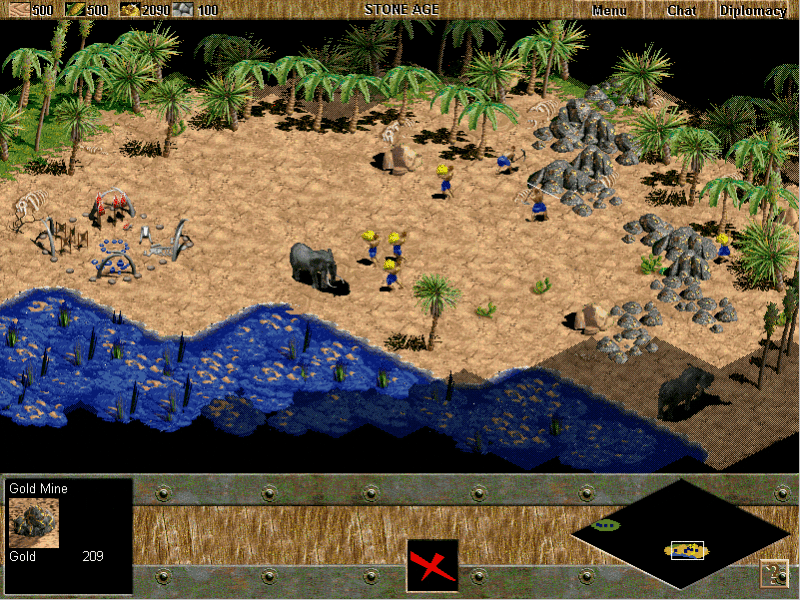
\includegraphics[width=300px]{0.bilder/aoe.png}
    \end{center}
    \caption{Screenshot aus Age of Empires (\cite{aoe})} \label{image:aoe}
\end{figure}
\subsection{Sid Meier's Civilization}
Das 1991 erschienene Spiel \textit{Sid Meier's Civilization} ist ein von \textit{MicroPose} entwickeltes und publiziertes, rundenbasiertes Strategiespiel \cite*[]{civigdb}. \textit{MicroPose} ist ein 1982 von Bill Stealey und Sid Meier gegründetes Softwareunternehmen, wovon von letzterem auch der Name abgeleitet wird \cite*[]{civhistory}. Man startet im Jahr 4000 B.C. und bewegt sich zeitlich bis ins Informationszeitalter, während man neue Städte gründet, Technologien erforscht und anderen Gegenspielern beziehungsweise Reichen und deren Herrschern begegnet, Diplomatie führt und gegebenenfalls auch Kriege. Unter den spielbaren Herrschern sind unter anderem \textit{Alexander der Große, Napoleon} und \textit{Julius Cäsar}. Das Spiel besitzt einen nicht-linearen Technologiebaum mit den wichtigsten Errungenschaften der Menschheit, darunter das Rad oder Navigation, verschiedene baubare Wunder, zum Beispiel die Pyramiden oder die Große Mauer und besitzt fünf verschiedene Schwierigkeitsgrade, mit denen der Spieler die Herausforderung selber setzen \cite*[]{civ}. Je nach Fokus des Spielers ist also jedes Match ein neues, und es gibt durch verschiedene Ressourcen und Entscheidungsmöglichkeiten einige Strategien denen sich der Spieler bedienen kann. \\
Das Spiel erhielt fünf weitere Nachfolger \textit{Civilization II, Civilization III, Civilization IV, Civilization V} und \textit{Civilization VI} \cite*[]{civall}, wobei sich manche Teile stark von anderen Unterscheiden, etwa in der Perspektive oder der Geometrie des Spielfeldes. So wurde von \textit{Civilization IV} auf \textit{Civilization V} das Spielfeld von einem \textit{Square Grid} auf ein \textit{Hex Grid} umgestellt \cite*[]{civallcompare}. Neben den Nachfolgern gab es einige Ableger, darunter \textit{Sid Meier's Civilization: Beyond Earth}, welches 2014 erschien und zwei Erweiterungen erhielt. Dieser Teil spielt, anders als alle anderen, auf einem fremden Planeten und hat eine Sci-Fi Thematik, statt wie üblich, eine historische \cite*[]{civbe}. Das Spiel besitzt, im Gegensatz zu allen anderen Nachfolgern, noch eine Vogelperspektive, statt wie später, eine isometrische (vgl. \autoref{image:civ}). Außerdem sind auch politische Auswahlmöglichkeiten wie Regierungen, oder religiöse Auswahlmöglichkeiten vorhanden. Die wichtigsten Eigenschaften sind in \autoref{table:civ} zusammengefasst.



\paragraph*{Siegbedingungen}
\begin{itemize}
    \item Alle Gegenspieler eliminieren mittels Militär
    \item Ein Raumschiff bauen und Alpha Centauri als erster erreichen
    \item Überleben bis die Zeit ausgelaufen ist \cite*[]{civwin}
\end{itemize}

\paragraph*{Ressourcen}
\begin{itemize}
    \item Kohle
    \item Fisch
    \item Wild
    \item Wild (Tundra)
    \item Edelsteine
    \item Gold
    \item Pferde
    \item Oasen
    \item Öl
    \item Robben
\end{itemize}\cite*[]{civ:ressources}
\newparagraph{Rezensionen}
\begin{tabularx}{0.8\textwidth} { 
    | >{\raggedright\arraybackslash}X 
    | >{\centering\arraybackslash}X 
    | >{\raggedleft\arraybackslash}X | }
    \hline
    IGDB & 93\% \cite*[]{civigdb}\\
    \hline
    AllGame & 5/5 \cite*[]{civ:review:allgame}\\
    \hline
    Game Informer & 8.5/10 \cite*[]{civ:review:gameinformer}\\
    \hline
    Next Generation & 4/5 \cite*[]{civ:review:nextgeneration}\\
    \hline
\end{tabularx}

\begin{table}[]
    \centering
    \caption{Civilization Eigenschaften (\cite*[]{civallcompare,civigdb,civwin, civ:ressources})}
    \label{table:civ}
    \begin{tabular}{|l|l|}
    \hline
    Erscheinungsjahr & 1991                                                                           \\ \hline
    Entwickler       & MicroPose                                                                      \\ \hline
    Publisher        & MicroPose                                                                      \\ \hline
    Multiplayer      & Nein                                                                      \\ \hline
    Ressourcen       & Kohle, Fisch, Wild, Wild (Tundra), Edelsteine, Gold, Pferde, Oasen, Öl, Robben \\ \hline
    Siegbedingungen  & Domination, Space Race, Time                                                   \\ \hline
    Spielbare Völker & 14                                                                             \\ \hline
    Perspektive      & Vogel                                                                          \\ \hline
    Technologien     & 67                                                                             \\ \hline
    \end{tabular}
\end{table}

\begin{figure}
    \begin{center}
        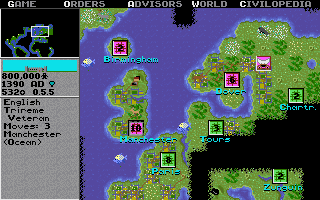
\includegraphics[width=300px]{0.bilder/civ.png}
    \end{center}
    \caption{Screenshot aus Civilization (\cite{civigdb})} \label{image:civ}
\end{figure}
\subsection{Sim City 2000}
Sim City 2000 ist ein im Jahr 1993 erschienenes Städteaufbauspiel für Einzelspieler, welches in das Genre \textit{Simulation} fällt \cite{simcity:ea}. Das Spiel wurde ursprünglich von \textit{Maxis} für den Mac entwickelt und publiziert, wurde in den kommenden Jahren jedoch für weitere Konsolen herausgegeben, darunter \textit{SNES, PlayStation} und \textit{Nintendo 64}. Im Jahr 2005 erschien es schließlich für den PC unter Windows \cite{simcity:igdb}. Der Spieler startet auf einer ausgewählten Karte, welche ein \textit{Square Grid} mit verschiedenen Höhen und Terrain besitzt. Die dabei zentrale Ressource ist Geld in Form von US Dollars. Der Spieler kann mit diesem Geld aus einer breiten Palette an Gebäuden wählen, darunter \textit{Schulen, Bibliotheken, Krankenhäuser} und \textit{Kraftwerke} \cite*[]{simcity:igdb}, welche die Bedürfnisse der Einwohner befriedigen und für Recht und Ordnung in der Stadt sorgen. Diese Gebäude besitzen einen Radius, was ein weiteres strategisches Element dieses Spiels darstellt, da auf möglichst sinnvolles Platzieren der jeweiligen Gebäude geachtet werden muss. Für Wohn-, Industrie- und Kaufhausgebäude markiert der Spieler Zonen, statt die Gebäude einzeln zu setzen. Die Gebäude dieser Zonen werden dann, je nach Bedarf, Stück für Stück aufgebaut oder wieder verlassen. Der Bedarf jeweiliger Zonen ist in \autoref{image:simcity} anhand des grünen (Wohngebäude), des blauen (Kaufhausgebäude) und des gelben (Industriegebäude) Balkens am linken Auswahlbalken erkennbar. Zeigt ein Balken dabei in die Richtung des \textit{+}, so signalisiert das \textit{Bedarf}, zeigt der Balken jedoch in die Richtung des \textit{-}, ist \textit{Überschuss} vorhanden. Zwischen diesen Zonen herrscht eine Relation, so benötigen Kaufhausgebäude die Industriegebäude als Produktionsquelle, und Wohngebäude als Käufer. Die Wohngebäude wiederum benötigen Arbeitsplätze, sowohl in Kaufhausgebäuden als auch in Industriegebäuden. Die Industriegebäude benötigen die Arbeitskräfte der Wohngebäude und Abnehmer für die produzierte Ware in Form von Kaufhausgebäuden. Diese Relation wird wie folgt berechnet (R:C:I beschreibt die Relation zwischen Wohngebäuden zu Kaufhausgebäuden zu Industriegebäuden): 
\newpage
\begin{itemize}
    \item Unter 10.000 Einwohnern: R:C:I = 4:1:3
    \item Zwischen 10.000 und 60.000 Einwohnern: R:C:I = 4:2:2
    \item Über 60.000 Einwohner: R:C:I = 4:3:1 \cite*[]{simcity:somacon}
\end{itemize}
Die Wohngebäude brauchen \textit{Strom, Wasser, Bildung, Sicherheit} und \textit{Freizeitaktivitäten}, welche allesamt durch platzierbare Gebäude gegeben werden können. Bildung ist eine Kernkomponente des Spiels, denn je nach Bildungsgrad der Stadt steigt oder fällt die Kriminalitätsrate und entscheidet auch darüber, welche Industrien blühen oder bankrottgehen. Der Bildungsgrad wird gemessen am EQ (\textit{education quotient}), so erhöht beispielsweise eine Schule den EQ von den 5 bis 20 Jahre alten Bewohnern. Es gibt insgesamt 156 Gebäude, welche in 8 Kategorien eingeteilt werden können, darunter verschiedene Arten von Wohngebäuden, Kaufhausgebäuden oder Industriegebäuden, wie auch verschiedene Parks, Statuen oder Kraftwerke \cite*[]{simcity:fandom}. \\
Ein weiteres zentrales Element des Spiels ist das \textit{Budget}, welche am Ende jedes Spieljahres adjustiert werden kann. So kann man die \textit{Steuern} erhöhen, die die Einwohner zahlen müssen, wie auch die \textit{Ausgaben} für verschiedene Institutionen anpassen. So kann beispielsweise das Budget der Polizei verringert werden oder das Budget der Feuerwehr erhöht werden, woraus jeweils Effektivitätsboni oder -mali folgen \cite*[]{simcity:video}. \\
Das Spiel hat keine Siegbedingungen, die Ziele setzt sich der Spieler selber. Mögliche Ziele sind dabei eine möglichst schöne Stadt, eine Stadt mit möglichst vielen Einwohnern oder man spielt vor sich hin und versucht ein Problem nach dem anderen zu lösen. Auch wenn das Spiel an sich nicht gewonnen werden kann, gibt es dennoch einen Endzustand und eine Art Gewinnsequenz. Der Endzustand ist ein Game Over, bei dem der Spieler durch \$100.000 Dollar Schulden aus \glqq seinem Büro eskortiert wird\grqq, siehe \autoref{image:simcitygameover}. Die mögliche Gewinnsequenz, die einem Sieg am ehesten kommt, ist durch baubare Arkologien bedingt. Arkologien sind sich selbst erhaltende Städte mit einer hohen Bevölkerungsdichte innerhalb eines meist hohen Gebäudes. Der Begriff wurde in den 50er Jahren von dem italienisch-amerikanischen Architekten Paolo Soleri geprägt, jedoch wurde bis heute noch keine echte Arkologie gebaut, auch wenn es dazu bereits einige Experimente, beispielsweise in Arizona, gibt \cite*[]{misc:arcology}. Nachdem der Spieler 301 sogenannte \textit{launch arcos} gebaut hat und das Jahr 2051 bereits angebrochen wurde, erscheint dem Spieler eine Nachricht, in Englisch \textit{\glqq The Exodus has begun\grqq}, woraufhin alle gebauten Arkologien explodieren und dem Spieler suggeriert wird, die Schiffe wären aufgebrochen, um neue Planeten zu besiedeln \cite*[]{simcity:arcology}. \\
Auch wenn das Spiel ein reines \textit{Singleplayer} Game ist, also lediglich ein menschlicher Spieler gleichzeitig spielen kann, spielt man dennoch gegen max. vier weitere Computerspieler, auch genannt \textit{KIs} (Künstliche Intelligenzen). Die maximal vier weiteren angrenzenden Karten der jeweils zu Anfang ausgewählten Karte werden von \textit{KIs} besiedelt und ebenfalls bebaut. Diese Nachbarstädte können mittels gegebener Transportmöglichkeiten, zum Beispiel Flugzeug oder Zug, Gewinn bringen, da die Bewohner der Nachbarstädte in beispielsweise den Kaufhäusern Geld ausgeben \cite*[]{simcity:manual}. \\
Eine weitere Eigenheit des Spiels sind die sogenannten \textit{Katastrophen} beziehungsweise \textit{Desaster}. Diese können vom Spieler komplett ausgeschaltet werden, falls gewollt. Die meisten Desaster können zufällig und natürlich passieren, darunter Feuer, Aufstände oder Fluten. Alle Desaster können ebenfalls vom Spieler selbst initiiert werden, um die Grenzen der eigenen Stadt auf die Probe zu stellen. Manche Katastrophen sind verkettet, so können Aufstände zu Feuer führen, oder Erdbeben zur Explosion von Kernkraftwerken führen, welche wiederum zu Feuern und Aufständen führen kann \cite*[]{simcity:manual}.\\
Das Spiel hatte einen Vorgänger \textit{Sim City}, welcher bereits 1989 erschien, und erhielt neun Nachfolger, darunter \textit{Sim City 3000, Sim City 4} und den neusten Teil \textit{SimCity: BuildIt}, welcher lediglich für mobile Endgeräte verfügbar ist und 2014 erschien. Der letzte Teil für den Computer erschien 2013 und trägt den Titel \textit{SimCity 2013} \cite*[]{simcity:timeline}. \\ Wichtige Eckdaten sind in \autoref{table:simcity} vorzufinden.

\paragraph*{Ressourcen}
\begin{itemize}
    \item Dollar
\end{itemize}
\newparagraph{Rezensionen}
\begin{tabularx}{0.8\textwidth} { 
    | >{\raggedright\arraybackslash}X 
    | >{\centering\arraybackslash}X 
    | >{\raggedleft\arraybackslash}X | }
    \hline
    IGDB & 78\% \cite*[]{simcity:igdb}\\
    \hline
    AllGame & 4.5/5 (PC) \cite*[]{simcity:review:allgame}\\
    \hline
    MacUser & 4.5/5 (Mac) \cite*[]{simcity:review:macuser}\\
    \hline
    Sega Saturn Magazine & 86\% (SAT) \cite*[]{simcity:review:segasaturn}\\
    \hline
\end{tabularx}

\begin{table}[]
    \centering
    \caption{Sim City 2000 Eigenschaften (\cite*[]{simcity:igdb})}
    \label{table:simcity}
    \begin{tabular}{|l|l|}
    \hline
    Erscheinungsjahr & 1993                                                                           \\ \hline
    Entwickler       & Maxis                                                                      \\ \hline
    Publisher        & Maxis                                                                      \\ \hline
    Multiplayer      & Nein                                                                           \\ \hline
    Ressourcen       & Dollars \\ \hline
    Siegbedingungen  & Keine                                               \\ \hline
    Endzustände  & Game Over                                               \\ \hline
    Perspektive      & Isometrisch                                                                          \\ \hline
    \end{tabular}
\end{table}

\begin{figure}
    \begin{center}
        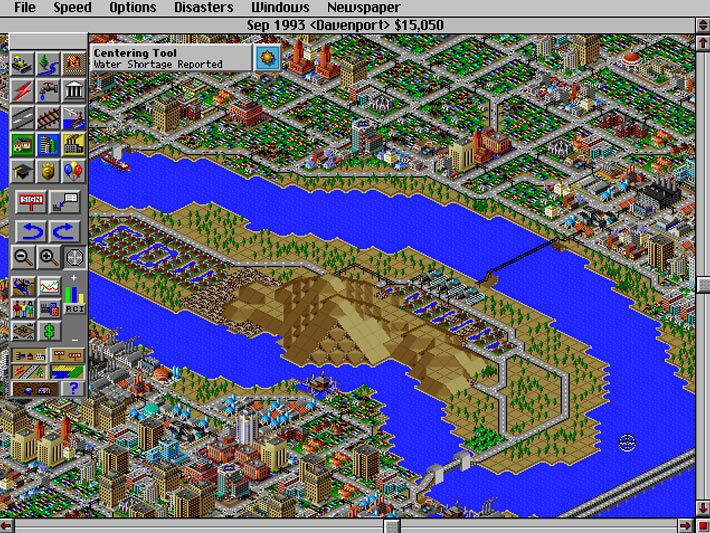
\includegraphics[width=300px]{0.bilder/simcity.jpg}
    \end{center}
    \caption{Screenshot aus Sim City 2000 (\cite{simcity:igdb})} \label{image:simcity}
\end{figure}
\begin{figure}
    \begin{center}
        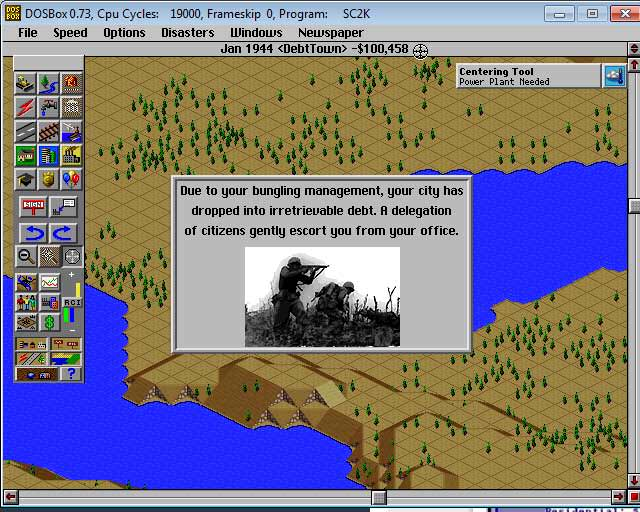
\includegraphics[width=300px]{0.bilder/simcityend.jpeg}
    \end{center}
    \caption{Game Over in Sim City 2000 (\cite{simcity:gameover})} \label{image:simcitygameover}
\end{figure}
\subsection{Weitere Beispiele}
Um den Überblick bestimmter Vertreter des Genres weiter auszubauen, werden im Folgenden weitere interessante Titel genannt, welche eigene Mechaniken innehaben und damit das Genre vorantreiben. Es ist 

\paragraph*{Factorio} Ein im August 2020 erschienenes Strategiespiel, welches von \textit{Wube Software LTD.} entwickelt und publiziert wurde \cite*[]{igdb:factorio} und einen großen Fokus auf Automatisierung und Effizienz legt. Der Spieler beginnt mit dem manuellen Abbau von Ressourcen, und beginnt allmählich primitive Prozesse zu automatisieren mittels Fliesbänder, Öfen und Kisten. Es gibt dabei etliche Produktionsketten mit verschiedenen Tücken und Tricks welche automatisiert werden können und dem Spieler Freiraum für kreatives Denken geben. Nebenbei ist der Spieler der Gefahr von außerirdischen Kreaturen ausgesetzt, welche ab und an angreifen und gegen welche er sich verteidigen muss.

\paragraph*{Frostpunk} Das von \textit{11 bit studios} entwickelte und publizierte Strategiespiel \cite*[]{igdb:frostpunk} fokussiert sich auf das Überleben im Eis. Überlebende Menschen in einer komplett gefrorenen Welt versuchen, eine Stadt zu gründen. Die Tücke dabei ist die Temperatur. Im Kern der Stadt befindet sich ein Generator, welcher stetig mit Kohle betrieben werden muss, da sonst die Menschen der Stadt erfrieren. Ressourcen sind sehr begrenzt und können außerdem über Spähtrupps von der Außenwelt gefunden und zurückgebracht werden, falls diese die Reise überleben. Der Spieler wird immer wieder mit Schneestürmen konfrontiert, welche stetig härter und schwieriger werden. Die Bevölkerung besitzt außerdem ein Level an Moral, welches aufrechterhalten werden muss. Fällt die Moral unter einen gewissen Punkt, endet das Spiel.

\paragraph*{Warcraft III} Veröffentlicht im Jahr 2002, entwickelt und publiziert von \textit{Blizzard Entertainment} \cite*[]{igdb:warcraft}. Das Spiel stellt einen Meilenstein des \textit{Real Time Strategy} Genres dar, wobei man zwischen vier verschiedenen Völkern wählen kann, welche allesamt eigene Einheiten, Eigenschaften und Mechaniken bieten. Außerdem gibt es verschiedene Heldeneinheiten, welche Gegenstände aufsammeln und tragen können und diese damit verstärken.

\paragraph*{Siedler von Catan} Das 1995 erschienene Brettspiel ist bis heute ein gespieltes Gesellschaftsspiel, welches von \textit{Klaus Teuber} entworfen wurde. Das Spielfeld ist in Hexagone aufgeteilt und rundenbasiert, wobei jedes Hexagon einer bestimmten Ressource zugeordnet ist. Die Spieler bauen zwischen den jeweiligen Hexagonen Siedlungen und im Verlauf des Spiels auch Städte, um auf diese Ressourcen Zugriff zu erhalten. 


\section{Analyse}
Im Folgenden wird eine IST-Analyse des Spiels \textit{RimWorld} durchgeführt, um anhand eines Colony Management Games herauszufinden, welche Mechaniken und Eigenschaften dieses Spiel auszeichnen, und welche davon gegebenenfalls übernommen werden könnten für den Prototyp eines neuen Spiels. Dazu wird zu allererst das Spiel näher untersucht, darunter die Mechaniken, die Kernelemente und das User-Interface. Anschließend werden Leitfaden-Interviews durchgeführt, dessen Ergebnisse und Transkripte verwendet werden, um Hypothesen für den Prototypen aufzustellen. Diese Hypothesen werden letztendlich mit einer Umfrage geprüft und mit der Implementierung des Prototypen schlussendlich umgesetzt. 

\subsection{RimWorld}
Das Strategiespiel \textit{RimWorld} ist ein im Jahr 2018 erschienenes Sci-Fi \textit{Colony Management} Game und wurde von \textit{Ludeon Studios} entwickelt und publiziert. Im normalen Szenario startet man mit drei Überlebenden eines Raumschiffabsturzes und versucht seine Kolonie aufzubauen und am Leben zu halten. Das Spiel hat etliche Mechaniken und Tücken, und durch den \textit{AI Storyteller}, welcher eine Vielfalt an Events plant und durchführt, ist eine hohe \textit{replayability} gegeben. Dieser kann auf eine gewünschte Schwierigkeit gestellt werden, von friedfertig bis unfair. Nachdem man den gewünschten Storyteller ausgewählt hat kann man den Planeten generieren (vgl. \autoref{image:rimworld}) und seinen Startpunkt innerhalb der Spielwelt bestimmen (vgl. \autoref{image:rimworld2}).

\begin{figure}
    \begin{center}
        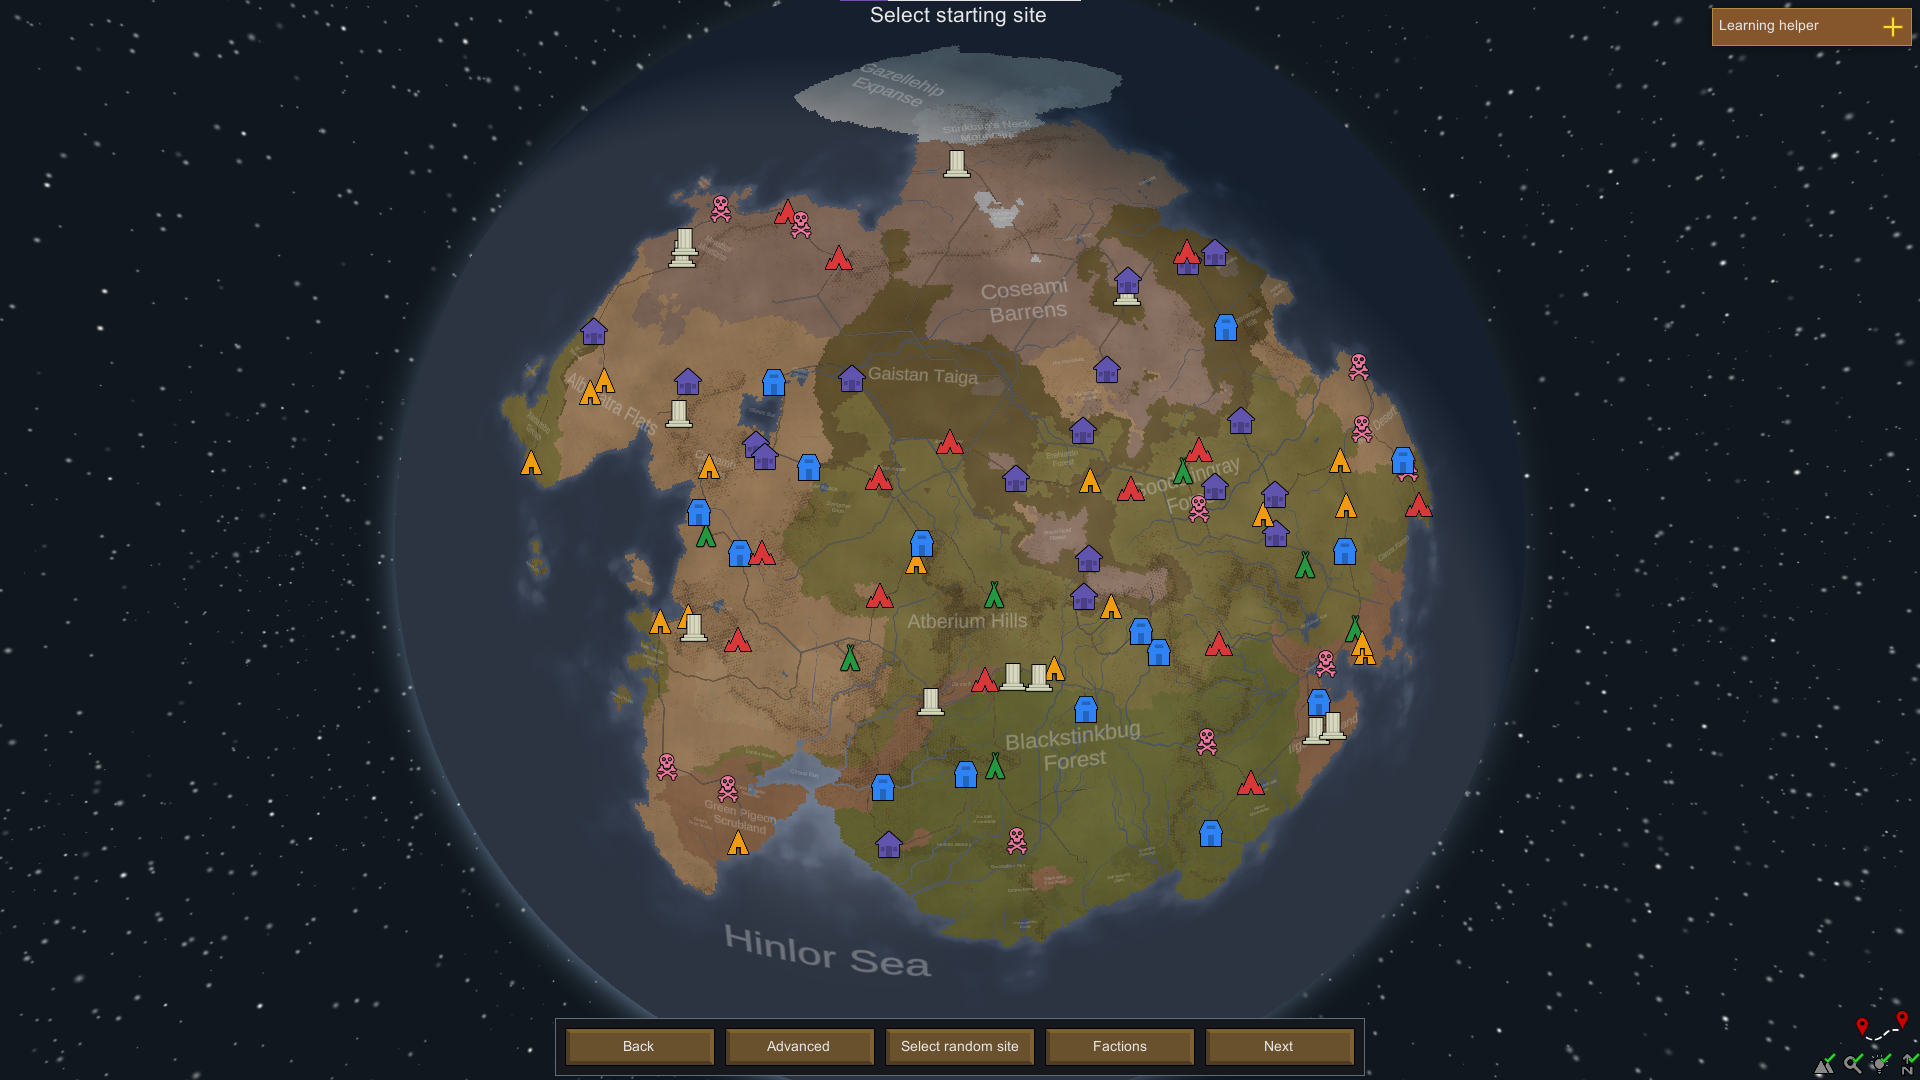
\includegraphics[width=300px]{0.bilder/rimworld.png}
    \end{center}
    \caption{Generierter Planet, Screenshot aus RimWorld} \label{image:rimworld}
\end{figure}

\begin{figure}
    \begin{center}
        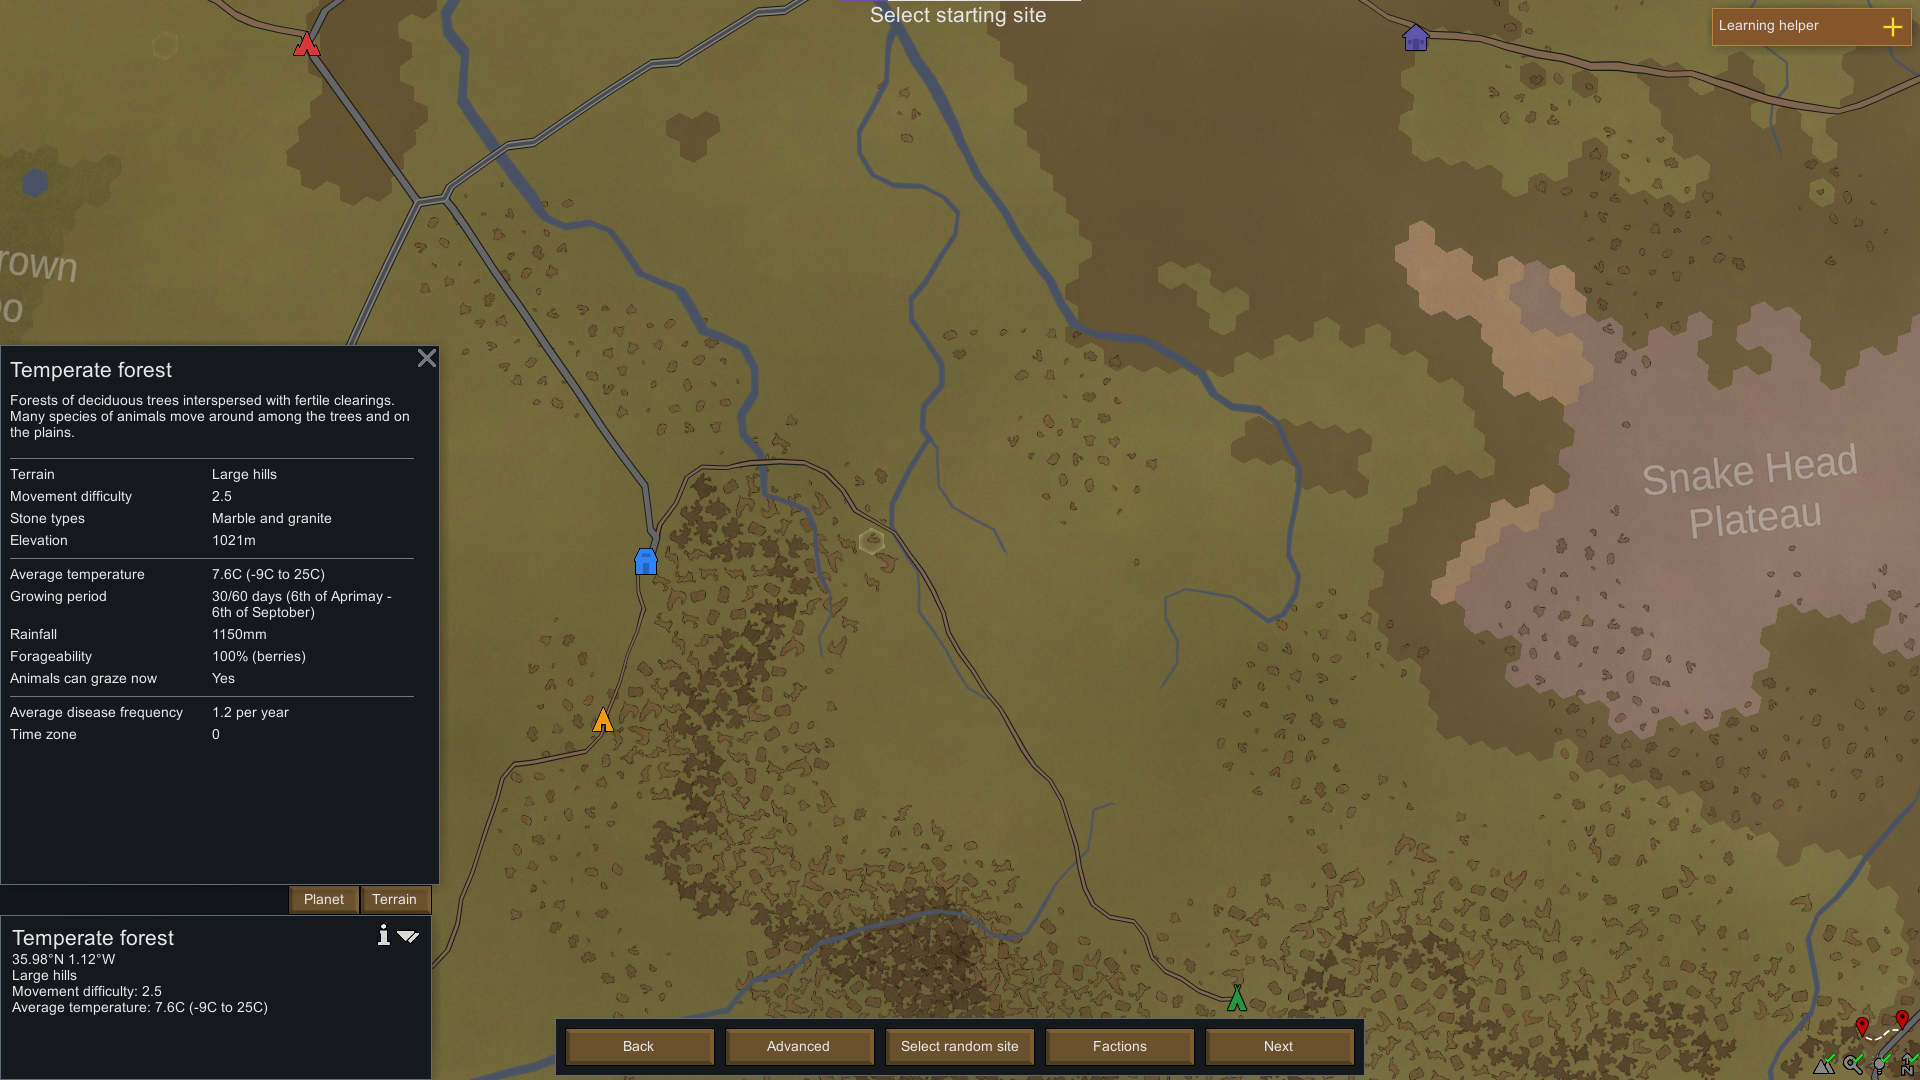
\includegraphics[width=300px]{0.bilder/rimworld2.png}
    \end{center}
    \caption{Ausgewählter Startpunkt für die Kolonie, Screenshot aus RimWorld} \label{image:rimworld2}
\end{figure}

\newparagraph{Spielwelt}
Die Welt ist für gewöhnlich eine Pangaea-artige Landmasse auf einem dreidimensionalen, blauen Planeten mit einem Äquator und einem Pol (vgl. \autoref{image:rimworld}). Der Planet ist aufgeteilt in hexagonale Kacheln, welche jeweils eine Karte symbolisieren. Die Kacheln haben dabei jeweils verschiedene Eigenschaften, die dann auf der gesamten Karte, welche der Spieler aussucht, gelten. Auf \autoref{image:rimworld2} lassen sich am linken Rand die meisten Eigenschaften anzeigen. Darunter die Terrain-Eigenschaften, wie viel Berge es gibt und damit auch Erzquellen, welche Steinarten es gibt und die Höhe der Karte. Außerdem ist ein maßgeblicher Faktor die Extreme der Temperaturen, zu welchen Zeiten man Felder anbauen kann und wie viel Regen für gewöhnlich fällt. Der Name der Kacheln, in diesem Fall \glqq Temperate Forest\grqq, gibt außerdem Aufschluss darüber, wie bewaldet die Kachel ist. Je nach Distanz zum Pol oder Äquator ändern sich diese Eigenschaften. Außerdem besitzen manche Kacheln einen Fluss oder bestehen gänzlich aus Wasser oder Eis, oder haben eine Anbindung zu einer Straße (grau) oder einem Feldweg (braun). Wählt man eine Kachel aus und drückt auf \glqq Next\grqq\;am unteren Bildschirmrand, gelangt man in die Auswahl der Kolonisten.

\newparagraph{Kolonisten}
Das Herz des Spielgeschehens sind die Kolonisten, die, mit manchen Ausnahmen, ihre zugewiesenen Aufgaben erfüllen. Die drei Startkolonisten kann man so lange neu generieren, bis man zufrieden ist. Es gibt dabei mehrere Eigenschaften, die ein Kolonist mit sich bringt. Die darunter fundamentalsten Eigenschaften sind die \textit{Skills}, welche mittig in \autoref{image:rimworldcharacter} zu sehen sind. Es gibt 12 verschiedene Skills, wovon jeder Kolonist ein bestimmtes Level hat. Diese werden zwischen \textit{0 - 5} generiert, wonach noch die \textit{Hintergründe} (engl. \textit{backstories}) und \textit{Eigenschaften} (engl. \textit{traits}) der jeweiligen Kolonisten addiert werden \cite*[]{rimworld:colonist}. Manche Hintergründe addieren oder subtrahieren Level von Skills, manche machen manche Tätigkeiten und damit einhergehende Skills auch unmöglich, darunter der Hintergrund \textit{Romanschriftsteller} (engl. \textit{novelist}), welcher es dem Kolonisten unmöglich macht, einfache Arbeiten zu erledigen, etwa Putzen oder Gegenstände umhertragen \cite*[]{rimworld:backstories}. Eigenschaften sind analog zu den Hintergründen zufällig generiert, beziehen sich größtenteils jedoch auf soziale Interaktionen oder bringen bestimmte Boni oder Mali für die \textit{Stimmung} des Kolonisten, darunter Sexualitäten, wie schnell der Kolonist lernen kann, oder exotischere Eigenschaften wie \textit{Kannibale} oder \textit{Psychopath} \cite*[]{rimworld:traits}. Die Flammen neben dem Level der Skills stehen für die \textit{Passion} des Kolonisten für bestimmte Skills. Ist keine Flamme neben dem Level zu sehen, so lernt der Kolonist diese Fähigkeit beim Durchführen davon mit einem Faktor von \textit{35\%}. Ist eine Flamme vorhanden, ist der Kolonist \textit{interessiert} und hat einen Lernfaktor von \textit{100\%}. Sind zwei Flammen vorhanden, \textit{brennt} der Kolonist für diese Tätigkeit und lernt mit einem Faktor von \textit{150\%}. Da viele verschiedene Tätigkeiten zu bestimmten Zeitpunkten ausschlaggebend für das Überleben der Kolonie sein könnten, kann es sinnvoll sein, eine breite Palette verschiedener Passionen und hochrangigen Skills zu haben. Ältere Kolonisten haben für gewöhnlich höhere Skills, sind jedoch davon öfter von \textit{Gesundheitsproblemen} betroffen, etwa Verlust von Seh- und Hörvermögen, oder langsamere Laufgeschwindigkeit. Außerdem haben manche Startkolonisten bereits zuvor gebildete \textit{Beziehungen} zu manch anderen, welche bestimmte Interaktionen vereinfachen oder erschweren.
 
\begin{figure}
    \begin{center}
        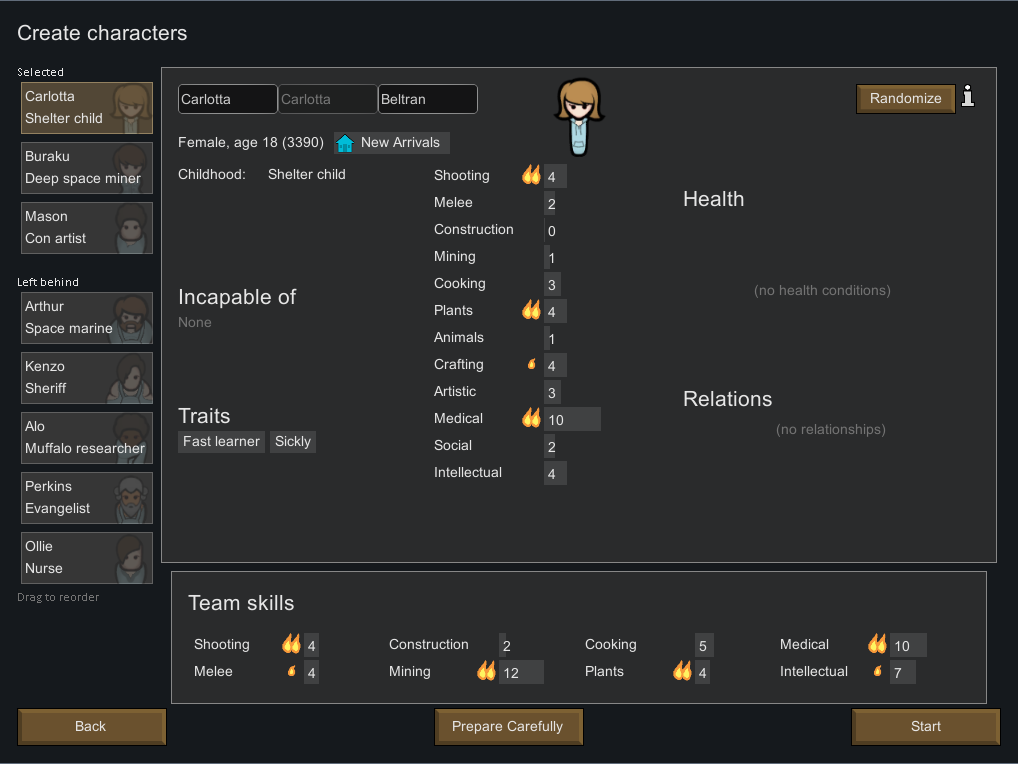
\includegraphics[width=300px]{0.bilder/rimworldcharacter.png}
    \end{center}
    \caption{Auswahl der Startkolonisten, Screenshot aus RimWorld} \label{image:rimworldcharacter}
\end{figure}

\newparagraph{Spielgeschehen}
Der Spieler wird nach der Anfangssequenz des Absturzes der Kolonisten nicht an die Hand genommen. Ein großer Teil des Spieles besteht darin, Strategien für das Überleben der Kolonie zu finden. Für gewöhnlich beginnt man damit, erste Teile der zukünftigen Basis zu bauen, wie diese aussehen soll und aus welchem Material diese besteht ist, wie so oft in diesem Spiel, dem Spieler selbst überlassen. Jeder Kolonist hat eine \textit{Stimmung} (engl. \textit{mood}), welche es gilt im Auge zu behalten (vgl. \autoref{image:rimworldmood}). Sollte die Stimmung zu lange zu niedrig sein, wird der Kolonist in einen nicht kontrollierbaren Zustand fallen, auch engl. \textit{mental break} genannt, wovon es verschiedene gibt. Darunter \textit{tantrum}, wobei der Kolonist alle möglichen Gebäude und Strukturen in seiner Sichtweite attackiert und möglicherweise zerstört, oder \textit{given up and leaving}, wobei der Kolonist die Spielerkolonie verlässt und aus dem Spiel entfernt wird \cite*[]{rimworld:mentalbreak}. Um diese Zustände zu vermeiden muss der Spieler sinnvoll die zu Anfang gegebenen Ressourcen nutzen, und für Nahrung, Unterschlupf, Wärme, Licht und etliche weitere Gegebenheiten sorgen. Je nach gewählten AI Storyteller passieren selten oder öfter Events, welche das Spielgeschehen maßgeblich beeinflussen können. Darunter sind \textit{raids}, wobei fremde Kolonien die Spielerkolonie angreifen, Gebäude zerstören, Reichtümer stehlen oder Kolonisten verschleppen, oder ein zufälliger Ansturm an Biebern, welche sämtliche Bäume auf der Karte Stück für Stück abholzen \cite*[]{rimworld:events}. Um gegebene Probleme zu Lösen kann der Spieler neue Technologien erforschen, welche letztendlich bis zum Bau eines Raumschiffes führen, was das vorprogrammierte Endziel des Spiels ist. Auf dem Weg zum Bau des Raumschiffes wird der Spieler also konstant vor neue Probleme, Launen der Kolonisten und Ressourcenmanagement gestellt, wodurch eine hohe replayability gegeben ist.

\begin{figure}
    \begin{center}
        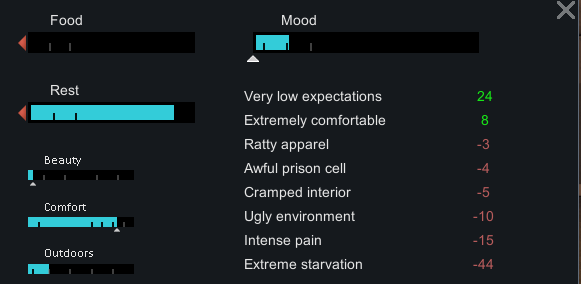
\includegraphics[width=300px]{0.bilder/rimworldmood.png}
    \end{center}
    \caption{Stimmungsbalken und -einflüsse, Screenshot aus RimWorld} \label{image:rimworldmood}
\end{figure}

\newparagraph{User Interface}
Das UI von RimWorld ist recht gefüllt, denn in jeder Ecke des Bildschirms finden sich direkt mehrere verschiedene Informationen, welche der Spieler erst kennenlernen und verstehen muss. Im Folgenden wird sich stark auf \autoref{image:rimworldui} berufen, anhand dessen das UI analysiert wird. Das UI ist zum besseren Verständnis in 13 verschiedene Stücke aufgeteilt, welche allesamt eigene Funktionen und einen bestimmten Mehrwert bieten. 

\begin{figure}
    \begin{center}
        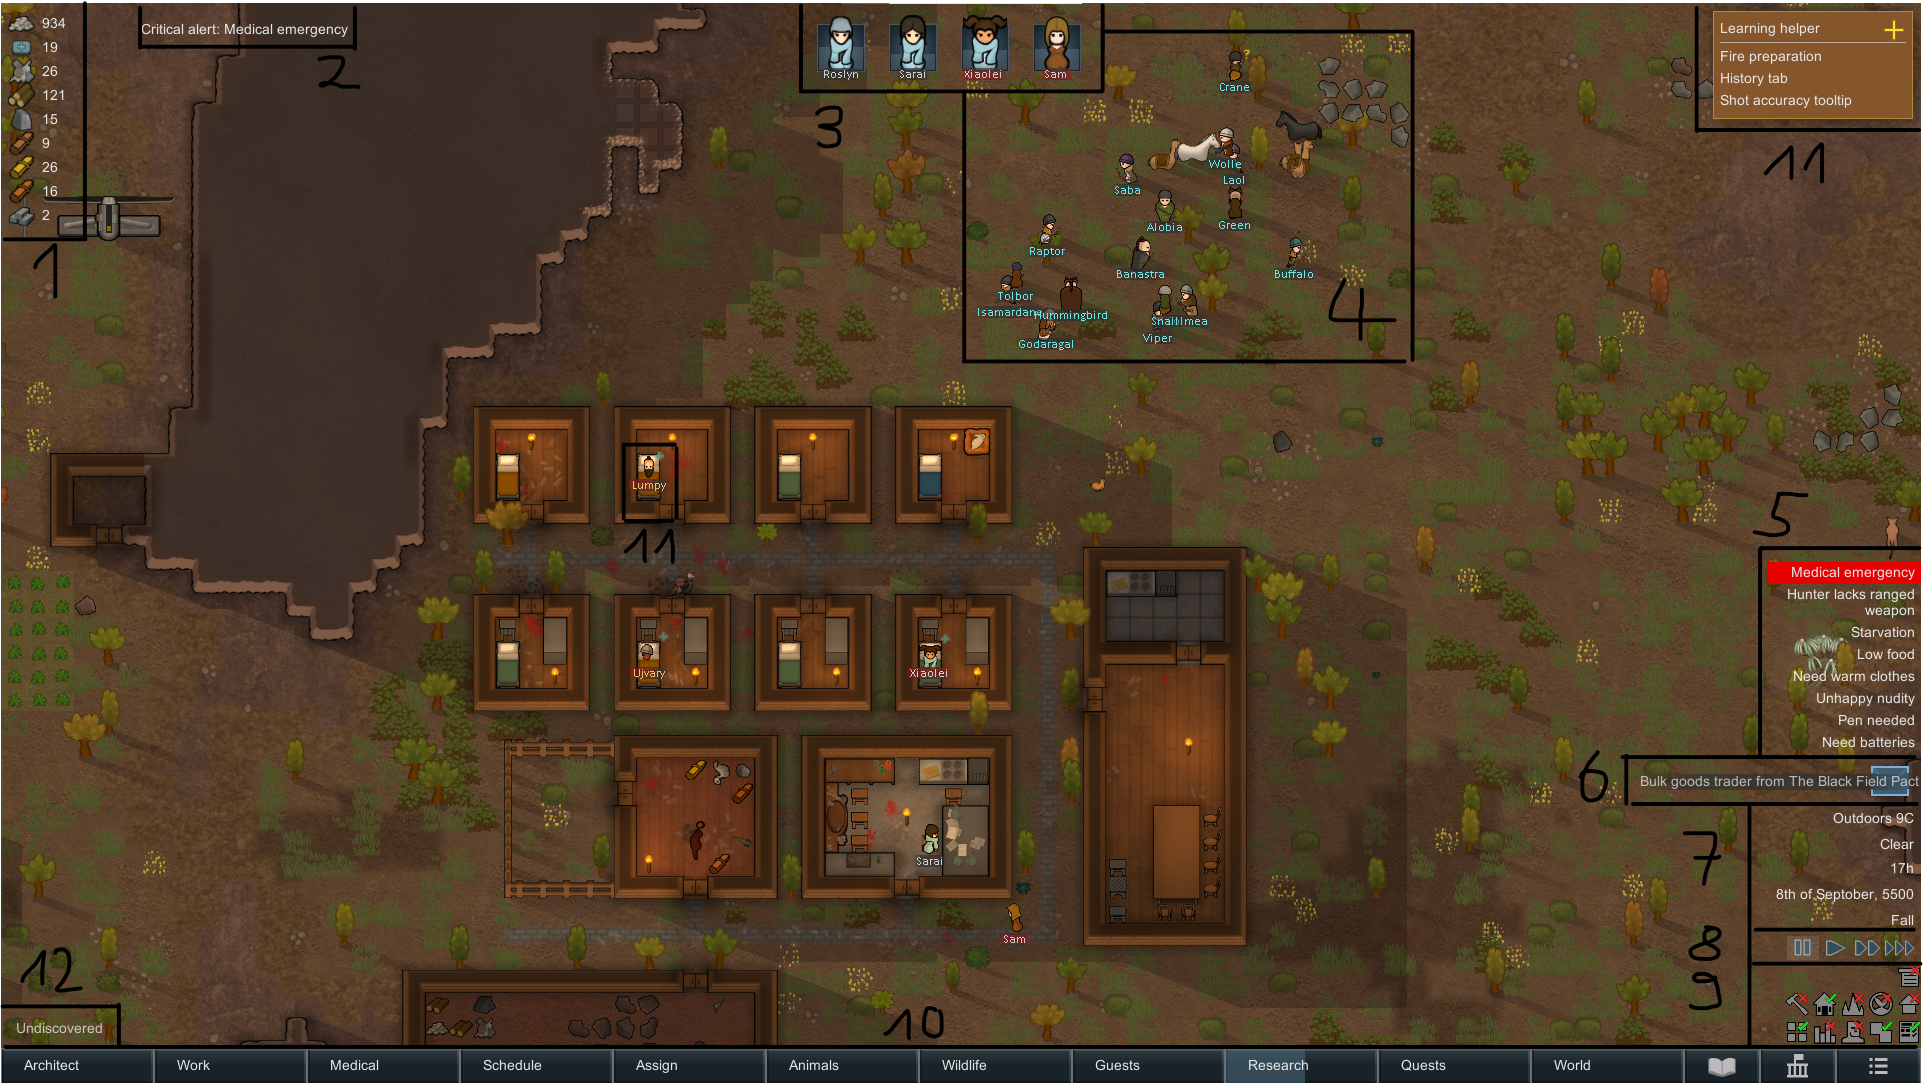
\includegraphics[width=400px]{0.bilder/rimworldui.png}
    \end{center}
    \caption{User Interface, Screenshot aus RimWorld} \label{image:rimworldui}
\end{figure}

Der erste Bereich des UI (1) zeigt die Ressourcen im Besitz des Spielers. Nicht alle Ressourcen werden vom Spieler besessen, sondern erst jene, die im definierten Lager vorhanden sind.
Der zweite Bereich (2) ist für kritische Meldungen, die sofortiges Handeln erfordern, in diesem Fall ein medizinischer Notfall, welcher zum Tod des Kolonisten führen kann.
In Bereich (3) werden alle Kolonisten, die Teil der eigenen Kolonie sind, angezeigt. Man kann dort sowohl Namen, als auch Aussehen, derzeitige Lebenspunkte und momentane Stimmung ablesen (hellblaue Füllung im Hintergrund des Quadrats).
Im vierten Bereich (4) ist gerade ein Event zu sehen, welches zufällig generiert wurde. In diesem Fall wird die Spielerkolonie von einer Händlerkarawane besucht, welche ein eigenes Inventar hat und mit dem Spieler handeln kann, also auch ein \textit{Händler} im Sinne einer ökonomischen Funktion.
Bereich (5) zeigt einige Zustände der Spielerkolonie an, darunter derzeitig hungernde Kolonisten, oder dass ein Jäger keine Waffe zum Jagen besitzt. Sehr dringende Zustände mit sofortigem Handlungsbedarf werden, wie in der Grafik zu erkennen, rot hinterlegt dargestellt.
In Bereich (6) werden ausschließlich vom AI Storyteller generierte Events mitgeteilt, also Hitzewellen, Angriffe oder, wie in diesem Fall, Besuche von Händlerkarawanen.
Im siebten Bereich (7) erkennt man meteorologische Informationen zu derzeitigen Wettergegebenheiten, der Temperatur, den derzeitigen Monat und die Jahreszeit.
Bereich (8) beinhaltet die Elemente zur Steuerung der Spielgeschwindigkeit.
Bereich (9) zeigt verschiedene Optionen zum Anzeigen bestimmter Informationen. Man kann sich beispielsweise noch die Fruchtbarkeitsgrade des Bodens einblenden lassen, oder die Schönheit der Umgebung aus der Sicht eines Kolonisten.
Der zehnte Bereich (10) stellt die Menüleiste dar, unter welcher man die meisten Aktionen im Spiel durchführen kann. Unter dem Reiter \textit{Architect} finden sich zum Beispiel Möbel und Strukturen (vgl. \autoref{image:rimworlduimenu}), welche man platzieren kann. Der am besten passende Kolonist wird dann dieser Tätigkeit zugeordnet. Bereich (11) zeigt einen im Bett liegenden Kolonisten, welcher zuvor verwundet wurde und sich nun regeneriert. Bereich (12) zeigt Informationen über das Element, auf welche die Maus gerade liegt. Dort können interessante Informationen bereitgestellt werden, zum Beispiel auf dem Boden befindlicher Dreck oder Blut, welches aufgeräumt werden sollte. Der letzte, nicht markierte Bereich ist der restliche Bereich des Bildschirms, wo sämtliches Spielgeschehen simuliert wird. Man erkennt den Anfang einer Kolonie, bestehend aus einigen Holzbaracken, einer Küche, einem Raum mit Tisch, um dort zu essen, ein kleines Lager und einen Produktionsraum, wo die Kolonisten die meiste ihrer Arbeit verrichten.

\begin{figure}
    \begin{center}
        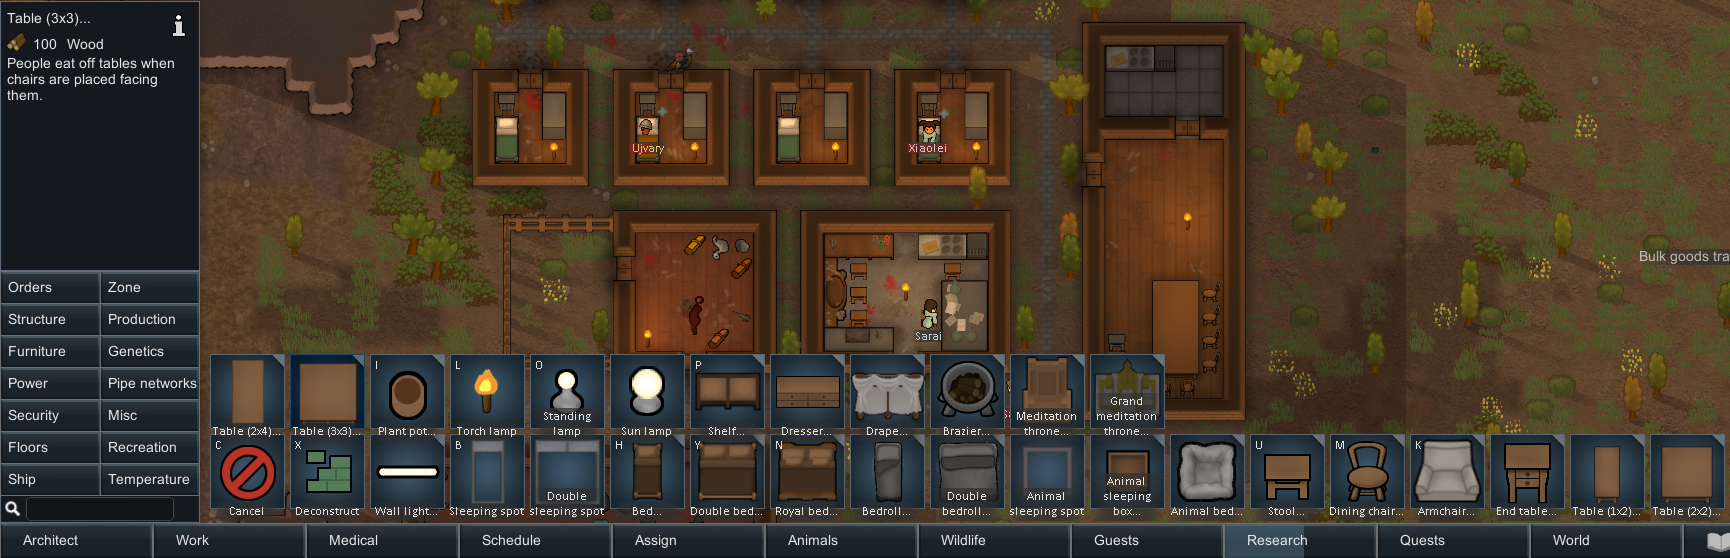
\includegraphics[width=400px]{0.bilder/rimworlduimenu.png}
    \end{center}
    \caption{Baumenü, Screenshot aus RimWorld} \label{image:rimworlduimenu}
\end{figure}

\newparagraph{Prioritäten}
Ein Großteil des Spielgeschehens läuft über die Prioritäten der Kolonisten. Man kann für jegliche mögliche Tätigkeit eine manuelle Priorität setzen (vgl. \autoref{image:rimworlduipriorities}), wodurch die Kolonisten erst bestimmte Tätigkeiten verrichten, bevor manch andere angefangen werden. Die Prioritäten reichen dabei von \textit{4} - niedrige Priorität, bis \textit{1} - hohe Priorität. Durch Linksklick auf ein Prioritätenfeld erhöht man die Priorität, durch Rechtsklick erniedrigt man sie. Man kann ebenfalls die Priorität auf \textit{nichts} setzen, wodurch die Tätigkeit unter keinen Umständen ausgeführt wird. Es kann daher sinnvoll sein, die Prioritäten höher zu setzen bei überlebenswichtigen Dingen wie Feuerlöschen oder medizinischer Hilfe, falls darin geübt.
\begin{figure}
    \begin{center}
        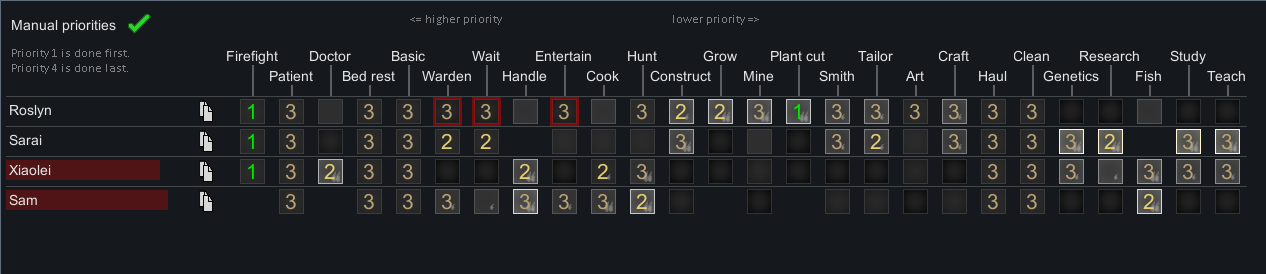
\includegraphics[width=400px]{0.bilder/rimworlduipriorities.png}
    \end{center}
    \caption{Prioritäten, Screenshot aus RimWorld} \label{image:rimworlduipriorities}
\end{figure}

\newparagraph{Steuerung der Kolonisten}
Anders als traditionelle Resource Management Games (Age of Empires, Civilization), steuert man seine Einheiten nicht \textit{direkt}, in dem man diese auswählt und dann auf das gewünschte Feld klickt, sondern \textit{indirekt}. Man wählt zuerst die auszuführende Tätigkeit aus der Liste der möglichen Befehle aus (vgl. \autoref{image:rimworldorders}), markiert den Bereich für den Befehl und der nächstbeste Kolonist, der diese Aufgabe erfüllen kann und die höchste Priorität dafür hat, wird zugewiesen sich darum zu kümmern. Das macht die zuvor genannten Prioritäten unerlässlich, um einen reibungslosen Spielverlauf zu haben. Der Vorteil dieser Mechanik ist ganz klar, dass sich das Management der Kolonisten eher anfühlt wie das einer Ameisenkolonie, statt dem herkömmlichen direkten Kommandieren der einzelnen Einheiten. Der klare Nachteil davon ist, dass man nicht immer die gewünschten Dinge erledigen lassen kann, die man gerade hätte. In manchen Situationen sind andere Tätigkeiten prioritär, wodurch man die Prioritäten stetig im Auge behalten muss und öfter mal anpasst, sodass auch wirklich das erledigt wird, was gerade notwendig ist.

\newparagraph{Ressourcen}
Das Spiel hat eine große Vielfalt an verschiedener Ressourcen. Darunter fallen Grundbedarfsgüter, wie eine einfache Mahlzeit, Heu oder Reis. Es gibt von einigen Rohstoffen allerdings verschiedenste Ausführungen, so hat beispielsweise Leder \textit{20} verschiedene Variationen (Schweinehaut, Hundeleder, Fuchsfell, \dots). Es gibt weiterhin sehr exotische Güter, zum Beispiel verschiedene bionische Körperteile, mit welchen man fehlende ersetzen kann, oder Nanobots, die fehlende Organe wiederherstellen können \cite*[]{rimworld:resources}. Es gibt eine Vielfalt an verschiedener, zubereitbarer Mahlzeiten, welche verschiedene Boni auf die Stimmung geben und jeweils verschiedene Rohstoffe benötigen.


\begin{figure}
    \begin{center}
        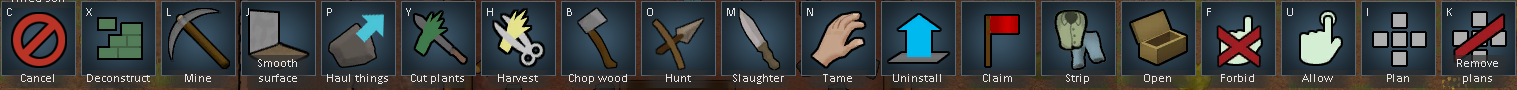
\includegraphics[width=400px]{0.bilder/rimworldorders.png}
    \end{center}
    \caption{Befehle, Screenshot aus RimWorld} \label{image:rimworldorders}
\end{figure}

\newparagraph{Haltbarkeiten}
Viele greifbare Ressourcen, welche auch in der realen Welt aufgrund von Korrosion zerstört würden oder als Lebensmittel mit der Zeit ablaufen, besitzen eine Haltbarkeit. Diese sinkt stetig mit vergehender Zeit von 100 auf 0. Ist diese auf 0 gesunken, verschwindet die Ressource aus dem Spiel, damit stellt diese Mechanik der Haltbarkeit ein Drain dar. Manche Ressourcen benötigen ein Dach oder einen Raum, damit die Haltbarkeit nicht weiter sinkt, andere wiederum und darunter primär Lebensmittel, benötigen eine sehr niedrige Temperatur, damit sie konserviert werden können.


\begin{figure}
    \begin{center}
        
\includegraphics[width=400px]{0.bilder/interviewphases.png}
    \end{center}
    \caption{Die Vier Phasen des Interviews} \label{image:interviewphases}
\end{figure}
\subsection{Interviews}
Für die Ermittlung gut funktionierender Mechaniken und Konzepte wird auf die Methode der nutzungsorientierten Gestaltung des kontextuellen Interviews zurückgegriffen \cite*[]{holtzblatt_beyer_1997}. Dazu wird ein Leitfadeninterview angefertigt, um qualitative Daten von den Teilnehmern zu extrahieren und daraus Hypothesen anzufertigen \cite*[]{baur_blasius}. Nachdem die Hypothesen erarbeitet wurden, werden diese mittels einer Umfrage in einem breiten Umfang überprüft. Es werden drei Personen ausgewählt, wobei die Erfahrung aller Personen in Bezug auf das Spiel und das Genre generell variiert. Diese Personen, im Folgenden auch \textit{Probanden} genannt, werden in Einzelgesprächen dazu gebeten, dass Spiel eine Stunde lang zu spielen. Einzelgespräche beziehungsweise -interviews sind Gruppengesprächen vorzuziehen, da die einzelnen Probanden einen entspannteren Zeitplan haben, sich gänzlich auf das Spiel und die Fragen fokussieren können und keine Gefahr laufen, abgelenkt zu werden oder mit anderen Probanden in Gespräche zu gelangen \cite*[]{lankoski_bjork}. Das Interview gliedert sich in vier Phasen (vgl. \autoref{image:interviewphases}).

\subsubsection{Versuchsaufbau}
Im Zentrum des Interviews steht, neben den Einleitungs- und Abschlussfragen, das Videospiel \textit{RimWorld}, welches für eine Stunde lang von den Probanden gespielt wird. Das Spiel läuft zu dem Zeitpunkt der Interviews auf der Version \textit{1.3.3387}, ist auf die englische Sprache eingestellt und wird über die Online-Vertriebsplattform für Computerspiele \textit{Steam} ausgeführt.
Das Interview ist, wie bereits erläutert, in vier Phasen gegliedert und wird in der Wohnung des Interviewers durchgeführt. Wichtig ist, dass alle Probanden leicht andere Qualifikationen besitzen, sodass ein breites Bild über den Zustand des untersuchten Spiels erstellt werden kann. Es ist fundamental zu erkennen, wie ein Spiel von Kennern, wie auch von Neulingen empfunden wird. Jedes Interview wird dabei mit einem Mikrofon aufgenommen und anschließend transkribiert. Die Transkripte sind wörtlich und nicht lautsprachlich angefertigt. Dies bietet den einfachen Vorteil, dass die später aufgestellten Hypothesen mit Textbelegen der Aussagen der jeweiligen Teilnehmer aufgestellt beziehungsweise belegt werden können. Allerdings werden die Namen der Teilnehmer nicht genannt und stattdessen durch ein Pseudonym ersetzt \cite*[S.97]{lankoski_bjork}. Alle angefertigten Transkripte sind im Anhang auffindbar, wovon für den kommenden Abschnitt \hyperref[transcript:A]{Transkript A}, \hyperref[transcript:B]{Transkript B} und \hyperref[transcript:C]{Transkript C} relevant sind.
 
\newpage
\paragraph {Einleitung}
Um die erhobenen Daten richtig kategorisieren zu können, werden als erstes grundlegende Daten zu der Person an sich erfasst:
\begin{itemize}
    \item F1: Wie alt bist du?
    \item F2: Nach welchem Geschlecht identifizierst du dich?
\end{itemize}

\paragraph{Aufwärmen}
Im zweiten Schritt des Interviews werden etwas spezifischere Fragen zu der Erfahrung und dem Verhalten bezüglich Videospielen gestellt:
\begin{itemize}
    \item F3: Hast du bereits Erfahrung in Videospielen?
    \item F4: Hast du bereits Erfahrung in Resource Management Games?
    \item F5: Hast du RimWorld bereits zuvor gespielt?
\end{itemize}

\paragraph{Beobachtung}
Die Phase der Beobachtung beschreibt die Spielphase. Der Proband wird dazu aufgefordert, das Videospiel \textit{RimWorld} zu spielen. Es ist von fundamentaler Wichtigkeit für diese Phase, das die beobachtende Person keinerlei Versuch unternimmt, sich in das Spielgeschehen oder das Verhalten der beobachteten Person einmischt. Es wird auch unterlassen, begangene Fehler aufzuklären oder in irgend einer anderen Art und Weise zu helfen, falls nicht anders möglich. Außerdem ist es wichtig zu erwähnen, dass nicht alle Fragen zwangsweise gestellt werden. Diese Fragen dienen lediglich als Katalog möglicher Fragen, die situativ gestellt werden können.

\begin{itemize}
    \item F6: Welche Emotion wird gerade verspürt?
    \item F7: Ist das Spiel für den Probanden immersiv?
    \item F8: Hat der Proband Verlustängste bezüglich der Kolonisten?
    \item F9: Wieso machst du \_\_\_?
    \item F10: Weißt du, was du nun tun kannst?
    \item F11: Was ist dein nächstes Ziel?
    \item F12: Verwendet der Proband die Prioritätenliste?
    \item F13: Kommt der Proband gut mit der indirekten Anweisungsmechanik zurecht?
\end{itemize}

\paragraph{Abschluss}
In der Abschlussphase wird der Proband gebeten, eine eigene Meinung abzugeben. Außerdem können Fehler aufgeklärt werden und inhaltliche Fragen beantwortet werden, ohne dass sie nun das Verhalten im Spiel verzerren.

\begin{itemize}
    \item F14: Was hast du als gut empfunden?
    \item F15: Was hast du als schlecht empfunden?
    \item F16: Wie findest du das indirekte Anweisen?
    \item F17: Was sagst du zu der Ressourcenvielfalt?
    \item F18: Was hältst du von dem Prioritätensystem?
    \item F19: Wie findest du die vielen zufällig generierten Umstände?
\end{itemize}

\subsubsection{Probanden}
Für die Interviews werden exakt drei Personen ausgewählt, welche sich allesamt in ihrer Erfahrung in Videospielen und auch in ihrer Erfahrung in RimWorld unterscheiden. Es ist damit zu erhoffen, dass ein möglichst breites Spektrum an Informationen extrahiert werden kann. Da Proband C sich zu dem Zeitpunkt des Interviews nicht vor Ort befand, wurde mit dieser Person stattdessen über Discord ein Meeting gehalten, in welchem der Bildschirm des Probanden dem Interviewer geteilt wurde. Der Prozess lief unwesentlich unkomplizierter ab, da beide Personen bereits vertraut mit der Software waren. 

% Please add the following required packages to your document preamble:
% \usepackage{graphicx}
\begin{table}[]
    \centering
    \caption{Jeweilige Antworten der Probanden auf die Einleitungsfragen}
    \label{table:interview}
    \begin{tabular}{|l|c|c|c|}
    \hline
                                  & Proband A & Proband B & Proband C \\ \hline
    Alter                         & 19        & 23        & 24        \\ \hline
    Geschlecht                    & \female        & \male         & \male        \\ \hline
    Erfahrung Videospiele         & $\upchi$      & \checkmark        & \checkmark        \\ \hline
    Erfahrung Resource Management & $\upchi$      & \checkmark        & \checkmark       \\ \hline
    Erfahrung RimWorld            & $\upchi$      & $\upchi$      & \checkmark       \\ \hline
    \end{tabular}
    \end{table}

\subsubsection{Ablauf}
Jegliches Interview beginnt mit den Einleitungsfragen, wobei die Antworten der Probanden zusammengefasst in \autoref{table:interview} zu finden sind. Die Altersspanne der Teilnehmer liegt zwischen 19 und 24 Jahren, mit einem Altersdurchschnitt von 22 Jahren. Zwei der drei Probanden sind männlich, ein Teilnehmer ist weiblich. Die beiden männlichen Teilnehmer weisen beide bereits Erfahrung in Videospielen und Resource Management Games auf, wobei lediglich einer der beiden männlichen Teilnehmer bereits RimWorld zuvor gespielt hat. Alle Teilnehmer wurden darüber in Kenntnis gesetzt, dass ihre Stimmen aufgezeichnet werden, und waren damit einverstanden. Die im Folgenden aufgestellten Hypothesen werden mit [HX] gekennzeichnet, wobei das X eine fortlaufende Nummerierung der jeweiligen Hypothesen darstellt. Die Referenzen auf die Transkripte werden mit [X, Z.Y] dargestellt, wobei X in diesem Fall das Pseudonym des jeweiligen Probanden ist (A, B, C), und Y die jeweilige Zeile in dem gegebenen Transkript.

Zu Beginn fällt auf, dass der Startbildschirm des Spiels sehr viele Buttons enthält, und die Option \glqq New Colony\grqq für Neulinge nicht unbedingt eindeutig assoziiert wird mit dem Beginn eines neuen Spiels [A, Z.27-30]. Es wäre daher sinnvoll, die Anzahl der Knöpfe auf ein Minimum zu reduzieren [H1]. Die Steuerung und die einzelnen Symbole auf der generierten Weltkarte sind nicht eindeutig assoziierbar [A, Z.39-48][B, Z.38-54], eine gewisse, gut sichtbare Erklärung oberhalb der Weltkugel wäre eine hilfreiche Ergänzung [H2]. Für spezielle, stark herausfordernde Gegner oder Umgebungseigenschaften empfiehlt sich die Möglichkeit, diese auch ausstellen zu können [H3]. Das gibt dem Spieler mehr Kontrolle über mögliche Frustration [C, Z.37-40]. Außerdem fällt auf, dass, gerade für Neulinge, die englische Sprache in Videospielen etwas speziell sein kann. Diese Spiele enthalten Begriffe, welche im schulischen oder alltäglichen Kontext eher weniger auftreten und daher erst gelernt werden müssen. Es ist daher sinnvoll, möglichst viele Sprachen aufgrund der höheren Inklusion und den dadurch niedrigeren Frust zu implementieren [H4][A, Z.49]. Die Auswahl der Startkachel hängt scheinbar sehr stark mit der Erfahrung des Probanden zusammen, Proband A wählt den Startpunkt zufällig [A, Z.41-48], um möglichst schnell das eigentliche Spiel zu beginnen, während Proband B den Startpunkt abhängig von den benachbarten Fraktionen macht, da diese als positiv assoziiert werden [B, Z.56-59]. Proband C ist der einzige Proband, welcher sich die Eigenschaften der einzelnen Kachel anschaut und basierend auf konkreteren Informationen die Entscheidung fällt, darunter die Anbauzeit und die Terrain-Beschaffenheit [C, Z.43-44]. Dieser Lernprozess und die damit verbundene, gewonnene Erfahrung, ist nicht schlecht. Es lässt Raum für Verbesserung und Lerneffekte. Dem Spieler sollte daher nicht mitgeteilt werden, welche Kacheln sinnvoller wären, als andere [H5]. In der Auswahl der Kolonisten fällt auf, dass selbst Spieler, welche bereits Erfahrung in anderen Spielen des Genres haben, leicht überfordert mit der Anzahl und Diversität der Eigenschaften der Kolonisten haben können [B, Z.74-77]. Für den Umfang von RimWorld ergibt diese Entscheidung durchaus Sinn, jedoch ist wichtig zu erkennen, das hier gegebenenfalls unnötige Komplexität hinzugefügt wird, welche Spieler frustrieren kann. Daher sollten die Traits auf eine kleinere Menge reduziert werden und intuitiv benannt und gestalten sein, damit sowohl neue, als auch erfahrene Spieler dieses System als gut empfinden [H6]. Mit der Zeit entstehen eigene Taktiken, welche Traits gut und welche als schlecht empfunden werden [B, Z.67-71][C, Z.46-53], was eine durchaus positive Entwicklung ist. Es sollte daher nicht klar erkennbar sein, welche Traits die besten, und welche die schlechtesten sind, der Spieler sollte dies über Zeit und durch mehrfaches Ausprobieren lernen [H7]. Die in \autoref{image:rimworldui} in Bereich (5) dargestellten Hinweise auf den Zustand der Kolonie erweisen sich als sehr hilfreich, da jeder der drei Probanden diese als Informationsquelle verwendet [B, Z.82]. Es könnte daher hilfreich sein, kleine, nicht zu viel verratende, Informationen über negative Eigenschaften an den Spieler preiszugeben [H8]. Somit wäre der Spieler nicht komplett auf sich alleine gestellt, aber dennoch nicht an die Hand genommen, sodass ein Lernprozess stattfinden kann. Das Lagersystem in RimWorld scheint für den Großteil der Probanden nicht ersichtlich zu sein, Proband A findet keine Möglichkeit zu lagern, während Proband B erst nach einer sprachlichen Klärung des Begriffes \glqq Stockpile\grqq\; die Lagermechanik beginnt zu begreifen [B, Z.89-92]. Statt einem versteckten Lagersystem sollte das Lager deutlich ersichtlicher dem Spieler präsentiert werden, in Form einer baubaren Struktur, analog zu einer Kiste oder einem Ablageplatz [H9]. Eine weitere nicht ersichtliche Information ist die momentane Uhrzeit (vgl. \autoref{image:rimworldui}, Bereich (7)), welche zentraler dargestellt werden sollte [H10][B, Z.95-98]. Die Mechanik der Temperatur scheint für Proband B interessant zu sein [B, Z.98], wodurch eine analoge Mechanik eventuell für etwas mehr Komplexität sorgen könnte, ohne dabei mehr Erklärungsbedarf zu kreieren [H11]. Alle drei Probanden verstehen, dass Nahrung in irgendeiner Weise zubereitet werden sollte [A, Z.106-111][B, Z.107-111][C, Z.72-73], wodurch sinnvolle Converter-Mechaniken durchaus intuitiv sein können. Daher sollten Converter an einigen Stellen verwendet werden, um die Komplexität etwas zu erhöhen, ohne das Unverständnis des Spielers zu fördern [H12]. Es zeigt sich im Verlauf, dass die Steuerung der Kolonisten sehr unintuitiv sein kann, falls nicht anders bereits bekannt [A, Z.72]. Die Prioritätenliste, mit welcher die indirekten Anweisungen der Kolonisten optimiert werden können, wird von dem Großteil der Probanden nicht verwendet und teilweise auch falsch verstanden [A, Z.85-90][B, Z.127-128]. Das System der Prioritäten scheint positiven Anklang zu finden [A, Z.135][B, Z.155][C, Z.130-132], wodurch ein analoges System unbedingt implementiert werden sollte [H13], allerdings sollten die Nummern gegebenenfalls durch Symbole oder leichter zu verstehende Darstellungsmöglichkeiten ersetzt werden, welche keine Einbuße in der Komplexität darstellen, aber das Verständnis für neuere Spieler durchaus fördern können [H14]. Auch das indirekte Anweisen der Kolonisten wird größtenteils als positiv empfunden, und für den Anwendungsfall von RimWorld dem direkten Anweisen, wie zu finden in beispielsweise \textit{Age of Empires}, vorgezogen [A, Z.127][B, Z.155][C, Z.122-124]. Während dieses System bei neueren Spielern eher ein Gefühl von Machtlosigkeit auslöst [A, Z.129], schlägt diese Empfindung bei steigender Erfahrung in ein Gefühl von mehr Kontrolle und Vorausplanung [B, Z.160-161], und letztendlich in das positive Gefühl des Beobachtens eines eigenen \glqq Ameisenstamms\grqq [C, Z.123-124] um. Daher wird dieses System auf lange Sicht einen positiveren Effekt bringen, als die alternative des direkten Anweisens, und wird daher vorzugsweise implementiert [H15]. Allerdings sollte es Hinweise auf die Steuerung geben, um anfänglichen Frust zu vermeiden, und neuere Spieler direkt abzuholen [H16]. Es zeigt sich außerdem, dass die vielen, zufällig generierten Umstände, beginnend bei der Weltkugel, der Startkachel und den Kolonisten, tendenziell eher als positiv aufgefasst werden, auch wenn Anfangs etwas unübersichtlich [A, Z.139-134][B, Z.173-175][C, 133-136]. Laut Probanden erhöhe diese Zufälligkeit in vielerlei Hinsicht die replayability des Spiels. Es empfiehlt sich daher, eine ähnliche Struktur zu übernehmen, und eine zufällig generierte Karte, wie auch zufällig generierte Einheiten mit jeweils eigenen, distinkten Eigenschaften bereitzustellen [H17]. Für alle Probanden scheint das User-Interface in einigen Punkten undurchsichtig und unübersichtlich. Proband A empfindet die Menge an Text als sehr überwältigend und problematisch [A, Z.57], wodurch es sinnvoll sein könnte, einige Informationen eher als Bilder beziehungsweise Icons darzustellen, statt als Text [H18]. Proband B hat eher Probleme mit der Anordnung der dargestellten Informationen, darunter die bereits erwähnte Uhrzeit. Solche zentralen Elemente sollten daher sichtbarer dargestellt werden ([H10]). Eine frustrierende Eigenschaft des Spiels ist die teilweise zu stark anziehende Schwierigkeit, welche vermieden werden sollte bei der Implementierung des Prototypen. Die Schwierigkeit sollte schwer genug sein, damit das Gefühl einer Herausforderung entsteht, aber nicht zu schwer, sodass der Spieler sich teilweise auch zurücklehnen kann, und der Kolonie beim Arbeiten zuschauen kann, ohne stetig gezwungen zu sein, Input zu geben [H19][C, Z.114-119]. Letztendlich ist ein Tutorial für das Erlernen des Spiels unerlässlich aufgrund der vielen gegebenen Informationen [A, Z.121-124][B, Z.143-145]. Es gibt dabei verschiedene Möglichkeiten, ein Tutorial zu implementieren, aber dem Spieler sollte jederzeit eine Art Hilfestellung zur Verfügung stehen, damit kein Gefühl von Stagnation oder Frustration entsteht aufgrund fehlender Informationen [H20]. Zuletzt scheint die Kontrolle über die Geschwindigkeit des Spiels als essenzieller Bestandteil, sowohl Proband B [B, Z.78-81] als auch Proband C greifen darauf häufig zurück, lediglich Proband A sieht darin keinen Nutzen [A, Z.77-79], wobei dieser Nutzen mit der Erfahrung in Videospielen generell erkennbar wird. Demnach sollte eine solche Zeitkontrolle ebenfalls implementiert werden, um die Kontrolle des Nutzers zu erhöhen [H21]. 

Die hier aufgestellten Hypothesen sind zur besseren Übersicht und für spätere Referenzen in \autoref{table:hypotheses} aufgelistet.
 

\begin{table}[]
    \centering
    \caption{Übersicht aller aufgestellten Hypothesen der durchgeführten Interviews}
    \label{table:hypotheses}
    \begin{tabular}{|l|l|}
    \hline
    H1 & Die Auswahlmöglichkeiten im Startmenü auf das Nötigste reduzieren         \\ \hline
    H2 & Steuerung und Optionen oberhalb der Weltkugel anzeigen                    \\ \hline
    H3 & Herausfordernde Umgebungseigenschaften an- und ausschalten können         \\ \hline
    H4 & Mehrere Sprachen unterstützen für eine höhere Inklusion und weniger Frust \\ \hline
    H5 & Keine Hilfe bei der Auswahl der Startkachel                               \\ \hline
    H6 & Traits intuitiv und Anzahl gering halten                               \\ \hline
    H7 & Traits nicht eindeutig im Nutzen vergleichbar machen                               \\ \hline
    H8 & Kleine Hinweise auf Probleme geben                              \\ \hline
    H9 & Lagerplätze als baubare Strukturen erkenntlicher machen                              \\ \hline
    H10 & Zentrale Informationen (Uhrzeit) kenntlicher darstellen                             \\ \hline
    H11 & Temperatur als mögliche Erweiterung der Komplexität                             \\ \hline
    H12 & Intuitive Converter als Erweiterung der Komplexität                             \\ \hline
    H13 & Prioritätensystem schafft mehr Kontrolle                             \\ \hline
    H14 & Prioritäten in Form von Grafiken erhöhen das Verständnis                             \\ \hline
    H15 & Das indirekte Anweisen der Kolonisten verstärkt das Spielgefühl positiv                            \\ \hline
    H16 & Die Steuerung sollte ersichtlicher sein   \\ \hline
    H17 & Zufällige Startbedingungen erhöhen die replayability                            \\ \hline
    H18 & Grafiken erhöhen die Übersicht im User-Interface                            \\ \hline
    H19 & Die Schwierigkeit muss sinnvoll zwischen herausfordernd und entspannt balanciert werden                            \\ \hline
    H20 & Es bedarf einem Tutorial und/oder Hilfestellungen auf Abruf                            \\ \hline
    H21 & Eine Zeitkontrolle ist eine sinnvolle Ergänzung                            \\ \hline
    \end{tabular}
    \end{table}
\subsection{Umfrage}
Die zuvor erarbeiteten Hypothesen sollten ursprünglich im Folgenden über die empirische Methode der Online-Umfrage überprüft werden \cite*[]{Evans2005TheVO}.  Die Online-Umfrage sollte auf \textit{Discord}-Servern durchgeführt werden. Discord ist ein soziales Medium, welches dazu dient Videos oder Videos auszutauschen, oder sich über Sprach- oder Textkanäle miteinander zu vernetzen und zu kommunizieren \cite*[]{discord:usage}. Discord hat 140 Millionen aktive Nutzer pro Monat, Tendenz stark steigend (Stand 2021) \cite*[]{discord:statistics}. Es gibt dabei mehrere \textit{Discord-Server}, welchen man mit einer Einladung beitreten kann, auf welchem sich mehrere Personen befinden, mit welchen man kommunizieren kann. Es gibt für RimWorld einen dedizierten Discord-Server, auf welchem sich (Stand 15.08.2022) 37.634 Mitglieder befinden. Bei der Erarbeitung ist jedoch ein entscheidender Punkt aufgefallen, welcher die Umfrage überflüssig macht: Discord-Server dieser Art werden im Normalfall tendenziell eher von Leuten betreten, welche bereits viel Kontakt mit dem Spiel haben oder hatten, und Informationen austauschen wollen. Da die Hypothesen zu einem entscheidenden Teil aus Annahmen bestehen, welche das Spielgefühl für Anfänger optimieren sollen, wäre der Raum, in welchem die Umfrage stattfinden würde, unangemessen. Ein erfahrener Spieler ist bereits an das User Interface gewöhnt, weiß, wonach und wohin er schauen muss und hat eigene Strategien für das Spiel entwickelt, wie das Interview mit Proband C gezeigt hat, was die Hypothesen großteils unbrauchbar macht.

\section{Prototyp}
Für den praktischen Anteil dieser Arbeit wird auf Grundlage der gewonnenen Erkenntnisse aus vorheriger Sektionen ein Prototyp angefertigt. Es wird also auf die Hypothesen zurückgegriffen, welche durch die Interviews und Umfragen erarbeitet und überprüft wurden. Außerdem wird anhand eines geeigneten Beispiels der Natur eine Thematik Stück für Stück untersucht und in Mechaniken transformiert. Konkret werden in Folgendem die Vorgänge innerhalb einer Bienenkolonie genauer beleuchtet, und erörtert, welche Elemente sich für ein Resource Management Game eignen. Der Prototyp wird versioniert mittels GitHub und ist jederzeit in Form eines \href{https://github.com/ProgFroz/hexabees}{Repositories} \cite*[]{repository} aufrufbar.

\subsection{Thematik}
Für den Prototypen bedarf es einer Thematik beziehungsweise einer Idee für das Gesamtkonzept. Dafür wurde die Idee einer \textit{Bienenkolonie} für interessant befunden. Bienen und deren Kolonien sind aus vielerlei Hinsicht geeignet als Thematik für den Prototyp, darunter der Fakt, dass Bienen bekannt dafür sind, Honig zu produzieren, wobei Honig eine konkrete Ressource darstellt. Im Kontext eines Resource Management Games und mit Rücksicht auf das zuvor untersuchte Spiel \textit{RimWorld} eignet sich jedoch am besten eine ganz spezifische Art der Bienen, die \textit{Honigbiene}, genauer gesagt die \textit{Westliche Honigbiene} (lat. \textit{apis mellifera}) \cite*[]{bees:name}. Grund dafür ist die Verhaltensweise von Honigbienen, da diese, anders als nahe Verwandte, stärker dazu tendieren, in Kolonien zu leben. Hummeln beispielsweise formen zwar auch Kolonien, aber deutlich kleinere und kürzer lebende. Die meisten Arten der Wildbienen jedoch sind tendenziell Einzelgänger. Eine weibliche Wildbiene legt ein Nest und versorgt ihren Nachwuchs mit Pollen und Nektar \cite*[]{bees:wild}. Somit bietet die Gattung der Honigbiene einige Vorgänge, welche sich in ein Colony Management Game umsetzen lassen. Dazu werden im Folgenden interessante Vorgänge und Eigenschaften der Gattung der Honigbiene genauer untersucht. Es ist zu erwähnen, dass der folgende Abschnitt nicht dazu dient, das gesamte Spektrum einer Bienenkolonie zu untersuchen, sondern lediglich Aspekte, die förderlich für die Entwicklung des Resource Management Games wären.

\subsubsection{Nahrung}
Eine Honigbiene ernährt sich primär von \textit{Nektar}, welchen sie von Blumen sammelt. Dieser Nektar ist zuckerhaltiger Saft, welcher von den Pflanzen ausgeschieden wird, um damit Insekten verschiedener Arten anzulocken. Dabei sind Sonnenblumen, Obstblüten, Löwenzahn und Raps besonders gute Nektarquellen \cite*[]{bees:food}. Eine weitere Möglichkeit um an energiereichen Zucker zu gelangen ist der sogenannte \textit{Honigtau}, welcher von einigen Insekten, darunter Blatt- und Schildläusen, ausgeschieden wird. Aus diesen beiden zuckerhaltigen Säften können die Bienen den \textit{Honig} produzieren, welcher ebenfalls als Nahrungsquelle dient, aber vor allem über die Wintermonate besonders wichtig ist, da Honig sehr lange haltbar ist \cite*[]{bees:honeywinter}. Der durch Honigtau produzierte Honig wird von Imkern als \textit{Waldhonig} gekennzeichnet \cite*[]{bees:food}. Saugt eine Biene den Nektar einer Blüte auf, gelangt dieser in den \textit{Honigmagen}. Dort kommt er in Kontakt mit verschiedenen Enzymen, welche den Nektar in \textit{Glukose} (Traubenzucker) und \textit{Fruktose} (Fruchtzucker) \cite*[]{bees:glucosefructose} aufspalten. Diesen biochemisch veränderten Nektar gibt die \textit{Sammelbiene} im Bienenstock an die sich dort befindlichen \textit{Arbeitsbienen} durch Auswürgen weiter, welche den Nektar erneut aufnehmen und auswürgen. Mit jedem dieser Prozesse wird der Nektar viskoser, wodurch allmählich Honig entsteht \cite*[]{bees:nectartohoney}.

Neben dem Nektar, dem Honigtau und dem Honig, welche primär als Quellen für Kohlenhydrate dienen, benötigen Bienen außerdem noch Quellen für Fette und Proteine. Dafür werden \textit{Pollen} verwendet, wobei Pollen die männlichen Geschlechtszellen einer Samenpflanze sind. Da die Samenpflanze mehr Pollen produziert, als für die Fortpflanzung nötig, können diese ohne Probleme von den Sammelbienen aufgenommen werden \cite*[]{bees:honeywinter}. Die Pollen werden in \textit{Pollenpaketen} aufbewahrt (vgl. \autoref{image:pollenpaket}), wobei Teile der aufgesammelten Pollen nicht in diesen Pollenpaketen landen, sondern an den Hinterbeinen haften bleiben. Besucht diese Sammelbiene nun eine weitere Blüte, werden diese Pollen abgestreift und der Fortpflanzungsmechanismus der Samenpflanze profitiert. Besonders pollenreiche Quellen sind dabei Obstbäume, Mohn, Mais, Klee und Raps \cite*[]{bees:honeywinter}.

\begin{figure}
    \begin{center}
        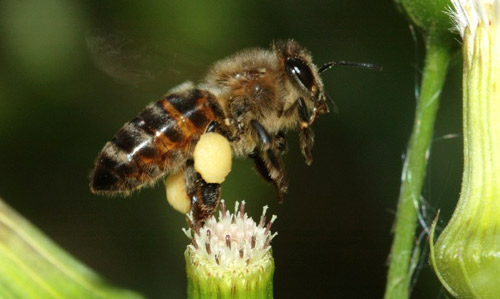
\includegraphics[width=300px]{0.bilder/pollenpaket.jpg}
    \end{center}
    \caption{Pollenpakete einer Honigbiene (\cite{bees:name})} \label{image:pollenpaket}
\end{figure}

Die letzte wichtige Ressource, welche Bienen für ihr Überleben benötigen, ist Wasser. Dieses kann von Flüssen oder Seen bezogen werden, wobei diese Quellen nicht mehr als 500 Meter weit vom Stock entfernt sein sollten. Erhalten Bienen nicht genug Wasser, können diese unter Verstopfungen leiden, was für das Überleben gefährlich sein kann \cite*[]{bees:honeywinter, bees:food}.

Es lassen sich somit wichtige Ressourcen identifizieren: \textit{Nektar, Honigtau, Honig, Pollen} und \textit{Wasser}. Außerdem ist die Aufteilung zwischen \textit{Sammel-} und \textit{Arbeitsbiene} eine mögliche Mechanik. Die Umwandlung von Nektar und Honigtau zu Honig könnte ebenfalls eine Mechanik darstellen, wie auch die naturgegebenen Quellen für Nektar, Honigtau und Pollen.

\subsubsection{Kasten}
Eine fundamentale Kategorisierung innerhalb einer Kolonie sind die \textit{Kasten}. Es gibt drei verschiedene Kasten beziehungsweise Arten von Bienen innerhalb solch einer Kolonie. Die erste Art ist die \textit{Bienenkönigin}. Diese Art der Biene ist genau ein mal vertreten und \textit{immer} ein Weibchen, zudem innerhalb einer Kolonie das einzige vollentwickelte. Die Hauptaufgabe der Königin ist das Brüten neuer Bienen und das Steuern des Schwarms mittels verschiedener Pheromone \cite*[]{bees:queen}. Die zweite Art sind die sogenannten \textit{Drohnen}. Diese Art ist \textit{ausschließlich männlich}. Diese Kaste ist lediglich zur Befruchtung der Königin da und ist nur von Frühling bis Sommer des Jahres in der Kolonie vertreten. Anschließend werden alle Drohnen gewaltsam aus der Kolonie entfernt, was als \textit{Drohnenschlacht} betitelt wird \cite*[]{bees:sex}. Die dritte und letzte Kaste der Kolonie sind die \textit{Arbeitsbienen}, welche, analog zur Königin, \textit{ausschließlich weiblich} sind, jedoch den deutlich größten Teil einer Kolonie ausmachen. Trotzdem legen diese Bienen in der Regel keine Eier, sind im Gegensatz dazu aber deutlich fürsorglicher gegenüber der Brut im Vergleich zur Königin. Die Arbeitsbienen sind prinzipiell für sämtliches weiteres Geschehen verantwortlich, darunter die Entfernung von Leichen oder die Nahrungsbeschaffung \cite*[S.2-3]{bees:frisch}. In \autoref{image:castes} werden die verschiedenen Kasten morphologisch unterscheidbar dargestellt mit einer Markierung verschiedener Merkmale. 

\begin{figure}
    \begin{center}
        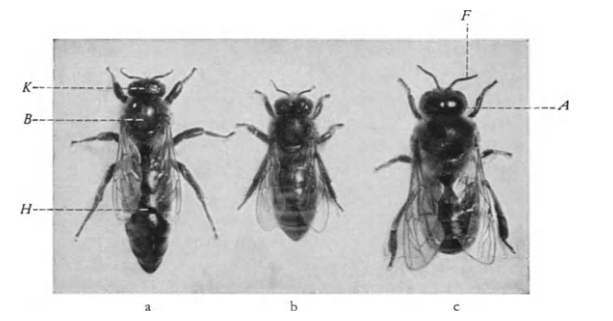
\includegraphics[width=300px]{0.bilder/castes.png}
    \end{center}
    \caption{(a) Königin, (b) Arbeitsbiene, (c) Drohne. (K) Kopf, (B) Brust, (H) Hinterleib, (A) Auge, (F) Fühler (\cite[S.2]{bees:frisch})} \label{image:castes}
\end{figure}



\subsubsection{Fortpflanzung}
Ein wichtiger Teil des Fortbestehens einer Kolonie ist die \textit{Vermehrung} beziehungsweise \textit{Fortpflanzung}. Wie bereits zuvor erwähnt gilt, dass sowohl Königinnen, als auch Arbeitsbienen jederzeit \textit{weiblich}, und Drohnen stets \textit{männlich} sind. Eine Königin ist in der Lage unbefruchtete Eier zu legen, oder diese Eier mittels Paarung mit Drohnen zu befruchten. Auch Arbeitsbienen sind in der Lage unbefruchtete Eier zu legen, was in einer Kolonie tendenziell selten passiert, da die Geschlechtsorgane der Arbeitsbienen zurückentwickelt und verkrümmt sind \cite*[]{bees:sex}. Wird allmählich eine neue Königin gebraucht, da die derzeitige Königin an das Ende ihres Lebens gelangt, sondert diese bestimmte Pheromone aus, wodurch dem Schwarm mitgeteilt wird, neue Königinnen heranzuziehen. Eine würde theoretisch ausreichen, aber um kein Risiko einzugehen werden mindestens \textit{sechs} Königinnen, oder mehr, versucht heranzuziehen. Nachdem eine geeignete Königin geschlüpft ist, werden die restlichen gewaltsam aus dem Schwarm entfernt \cite*[S.33]{bees:frisch}. Spätestens zwei Wochen später fliegt die neu geschlüpfte Königin aus und versprüht Pheromone, auch \textit{Königinnensubstanz} genannt, welche Drohnen eigener und fremder Völker anlocken, um sich mit der Königin zu paaren. Es wird mit maximal 12 Drohnen der Paarungsakt vollzogen, wobei die Königin bis zu \textit{zehn Millionen} Spermien aufnimmt, welche für die restliche Lebenszeit reichen \cite*[]{bees:queen}.

Einige Tage nachdem die Eier der zukünftigen Königinnen gelegt wurden, in der Regel neun Tage, beginnt der Akt des \textit{Schwärmens}. Dabei verlässt ein Teil der Kolonie, tausende von Bienen, zusammen mit der noch regierenden Königin den Schwarm, um sich auf die Suche nach einem neuen Zuhause zu machen und ein neues Bienenvolk zu gründen. Dieser Akt passiert in der Regel nur ein Mal pro Jahr, gegen Mai. \textit{Spurbienen} agieren als Späher und teilen Informationen über mögliche neue Heimatplätze. Laut Forschungen bedarf es 15 Spurbienen, welche dieselben Informationen über einen passenden Ort teilen, damit die Entscheidung gefällt wird \cite*[]{bees:swarm}. Dank der Pheromone der Königin bleibt der Schwarm während des Schwärmens stets zusammen \cite*[]{bees:queen}. 

Eine Königin besitzt einen \textit{diploiden} Chromosomensatz, dementsprechend \textit{2n = 32} Chromosomen. Die \textit{unbefruchteten} Eier werden von keinem zweiten Chromosomensatz ergänzt, wodurch die sich daraus entwickelnden Drohnen vorerst einen \textit{haploiden} Chromosomensatz besitzen, dementsprechend \textit{n = 16} Chromosomen in Summe. Diese werden jedoch nachträglich diploid, lediglich die Keimzellen bleiben haploid. Dadurch gilt, dass die anschließend diploiden Körperzellen der Drohne  \textit{homozygot} sind, da sie mittels \textit{Autopolyploidisierung} aus einer haploiden Eizelle entstanden sind. Beide Gene eines Merkmals stimmen also exakt überein \cite*[]{bees:homozygot}. Aus unbefruchteten Eiern schlüpfen ausschließlich Drohnen. Gegensätzlich dazu schlüpfen aus den \textit{befruchteten} Eiern Arbeitsbienen \textit{oder} Königinnen. Diese Eizellen sind durch die Beteiligung zweier Partien, der Königin und einer Drohne, sowohl \textit{heterozygot}, als auch diploid. Der Faktor, ob aus einem befruchteten Ei eine Arbeitsbiene oder eine Königin schlüpfen wird, ist modifikativ, also durch äußere Einflüsse, bestimmt. Der Unterschied liegt in der zugegebenen Nahrung der Maden in den ersten drei Lebenstagen. Während die zukünftigen Arbeitsbienen mit Pollen und Honig ernährt werden, erhalten die zukünftigen Königinnen ausschließlich \textit{Gelée Royal} (engl. \textit{Royal Jelly}) in ihren sogenannten \textit{Weiselzellen}, welche ausschließlich einer zukünftigen Königin vorenthalten sind \cite*[]{bees:swarm}. Somit gilt, dass Arbeitsbienen und Königinnen genetisch identisch sind, jedoch durch die zugegebene Nahrung modifikativ zu einer gewissen Kaste herangezogen werden können \cite*[]{bees:sex}. Es gilt also dass, auch wenn auf den ersten Blick paradox erscheinend, eine Drohne nie einen Vater, aber immer einen Großvater hat.

\subsubsection{Metamorphose}
Der Vorgang der \textit{Metamorphose} beschreibt das Anpassen der physischen Form oder ein plötzliches Ändern der äußeren Erscheinung \cite*[]{bees:metamorphosisdefinition}. Bienen durchlaufen vier verschiedene Zustände der Metamorphose, beginnend als \textit{Ei} (engl. \textit{egg}). Diese Eier werden von der Königin in eine leere Wabe gelegt, haben eine Größe von 1mm bis 1.5mm und ähneln einem Reiskorn. Nach circa \textit{drei Tagen} brechen die Eier und eine \textit{Larve} (engl. \textit{larva}) kommt hervor. Diese Larve ist weiß und C-förmig (vgl. \autoref{image:metamorphosis}). Die Dauer der kommenden Metamorphose hängt von der jeweiligen Kaste der zukünftigen Biene ab, Arbeitsbienen benötigen 6 Tage, Drohnen 6.5 Tage und Königinnen 5.5 Tage. Ist die Larve reif für die Metamorphose, richtet sie sich auf, sodass die Arbeitsbienen, welche Zuständig für die Brut sind, die Zelle mit \textit{Bienenwachs} bedecken. Die Larve verhärtet und wird zu einer \textit{Puppe} (engl. pupa). Analog zum vorherigen Stadium ist die Dauer bis zur kommenden Metamorphose abhängig von der Kaste der zukünftigen Biene. Eine Arbeitsbiene benötigt 12 Tage, eine Drohne 14.5 Tage und eine Königin 8 Tage. Ist die Zeit reif und die Metamorphose abgeschlossen beißt sich die Biene durch das Bienenwachs der Zelle und gesellt sich zu ihren Artgenossen \cite*[]{bees:name}.


\begin{figure}
    \begin{center}
        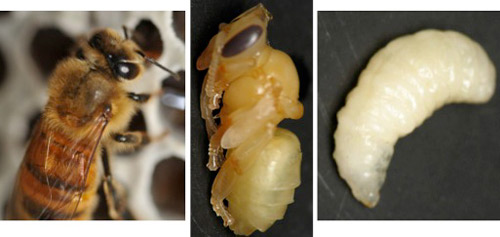
\includegraphics[width=300px]{0.bilder/metamorphosis.jpg}
    \end{center}
    \caption{Verschiedene Stadien einer Honigbiene, ausgewachsen (links), Puppe (mitte), Larve (rechts) (\cite[]{bees:name})} \label{image:metamorphosis}
\end{figure}

\subsubsection{Aufgabenverteilung}
Die Aufgaben der Königin und der Drohnen wurde zuvor bereits ausgiebig erläutert.
Eine Arbeitsbiene hat drei exakt eingeteilte Phasen ihres Lebens, in welchen verschiedene Tätigkeiten verrichtet werden. Die zu erledigenden Aufgaben sind also direkt gekoppelt an das derzeitige Alter einer Arbeitsbiene. Der erste Lebensabschnitt ist zwischen dem 1. und 10. Lebenstag der Biene. In diesem Stadium wird die Biene als \textit{Hausbiene} bezeichnet, da sie sich 
ausschließlich innerhalb des Bienenstocks aufhalten. Dort reinigen sie die Zellen, kümmern sich um die Brut als sogenannte \textit{Brutamme} und sind ansonsten meist untätig. Der zweite Lebensabschnitt findet zwischen dem 10. und 20. Lebenstag der Biene statt. In diesem Abschnitt wird die Biene als \textit{Baubiene} eingestuft. Die Aufgaben sind nun primär das Entgegennehmen des von den Sammlern gebrachten Nektar oder der Pollen, das Bauen neuer Waben und das Herstellen von Wachs. Außerdem sind manche diese Bienen im \textit{Wächterdienst} und beschützen den Stock vor Eindringlingen wie Wespen, Pferden oder Menschen. Im dritten und letzten Abschnitt des Lebens sind die Bienen \textit{Sammlerbienen}, welche Nahrung für den restlichen Stock von der Außenwelt suchen. Allerdings gibt es nur Ausflüge, wenn das Wetter und die Temperatur passend sind. Bei Regen, Schnee oder generell im Winter sitzen diese Bienen im Stock und warten auf Veränderung der Außenbedingungen. In der Regel widmen diese Bienen sich nicht den anderen Aufgaben und warten stattdessen \cite*[S.42-44]{bees:frisch}. \autoref{image:livesofcastes} zeigt einen Überblick der jeweiligen Aufgaben abhängig von dem Alter einer Biene jeglicher Kaste.

\begin{figure}
    \begin{center}
        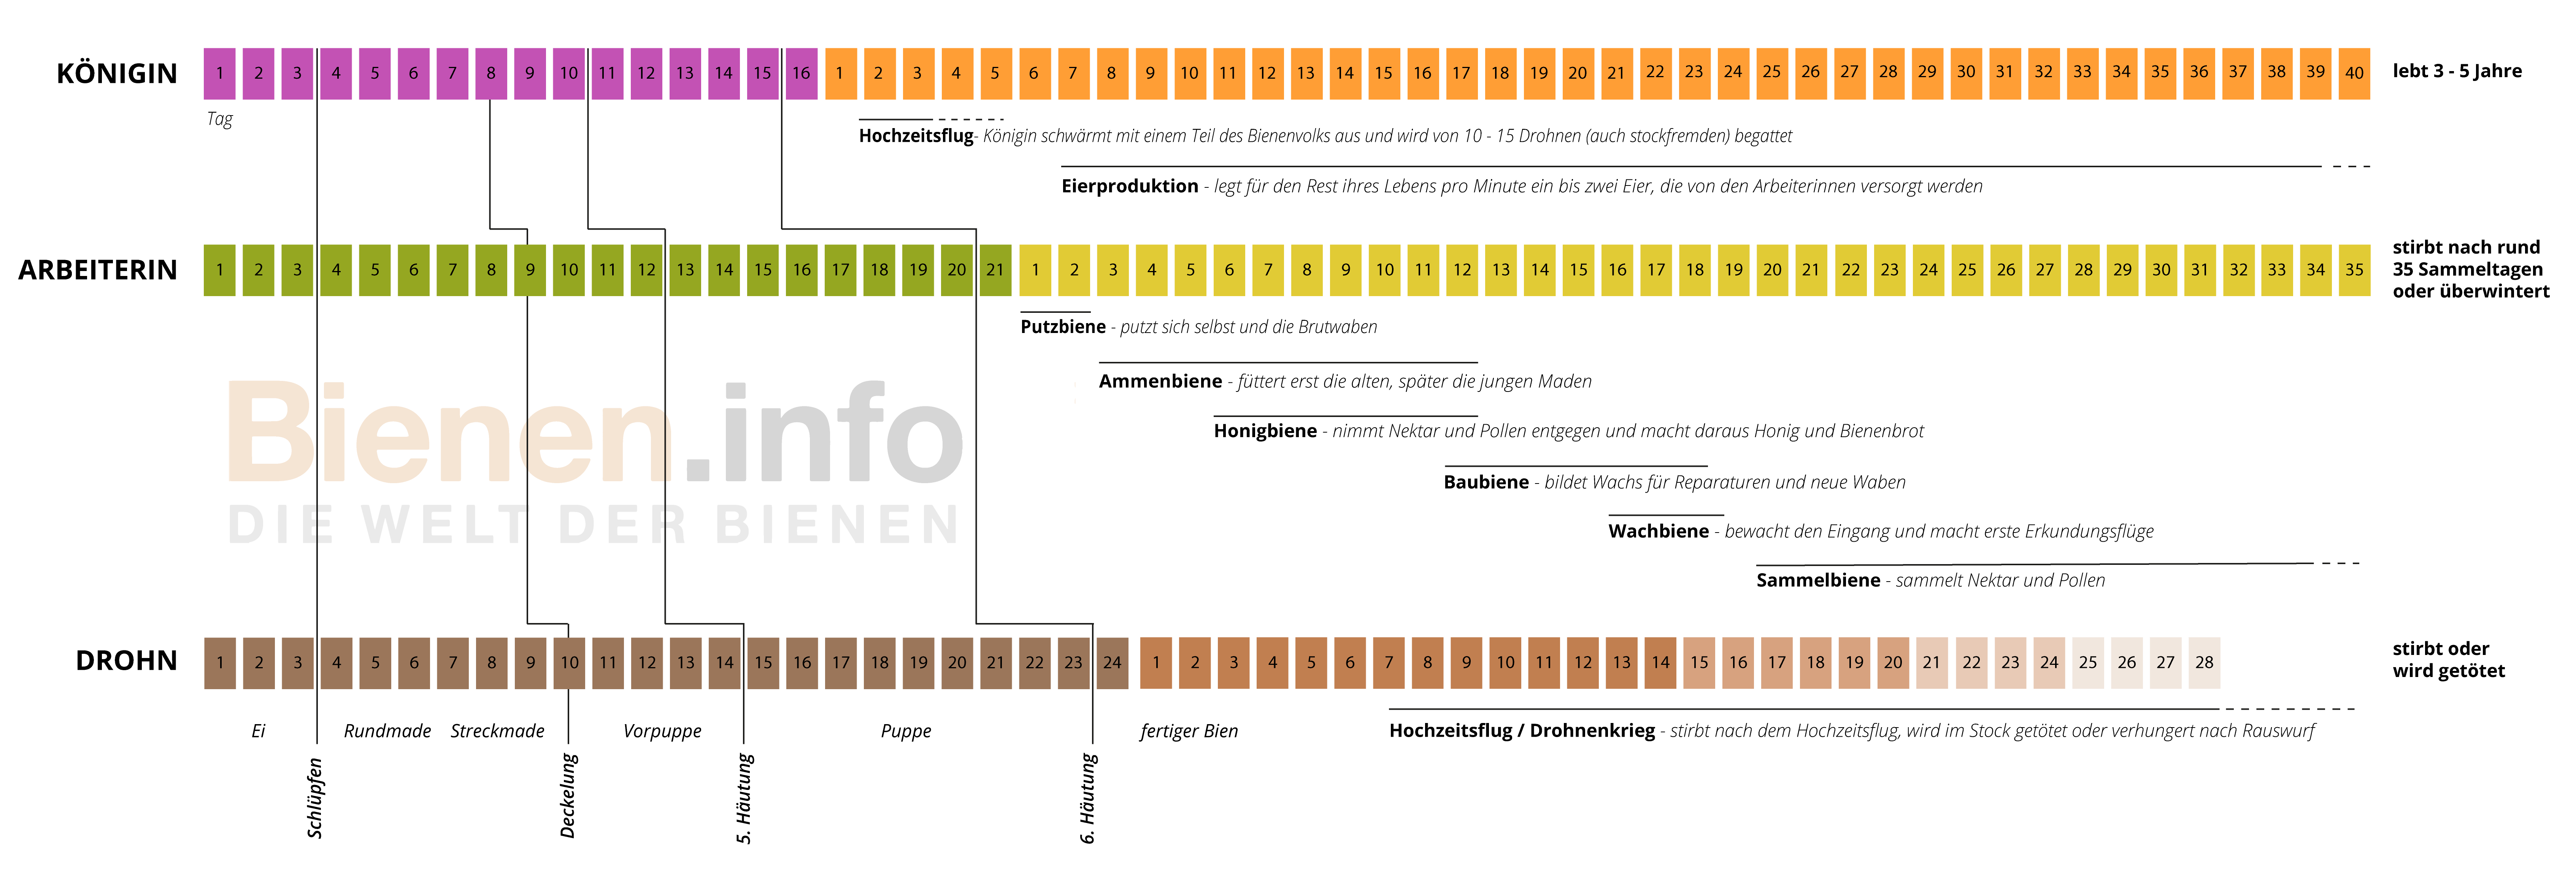
\includegraphics[width=400px]{0.bilder/livesofcastes.png}
    \end{center}
    \caption{Überblick über den Lebensverlauf einer Biene jeder Kaste (\cite[]{bees:lifeexpectancy})} \label{image:livesofcastes}
\end{figure}

\newpage
\subsubsection{Lebenserwartungen}
Die Lebenserwartung einer jeden Biene hängt mit ihrer jeweiligen Kaste zusammen. Die kürzeste Lebensdauer weisen die Drohnen auf, welche zwischen zwei bis vier Wochen leben, da diese anschließend durch die Drohnenschlacht gewaltsam entfernt oder getötet werden. Am längsten hingegen leben Königinnen, mit drei bis fünf Jahren Lebensdauer. Bei Arbeitsbienen ist es entscheidend, ob diese während des Sommers oder gegen Anbruch des Winters geschlüpft sind. Durch die Wintereinnistung steigt die Lebenserwartung der Arbeitsbienen stark an, von gerade mal zwei bis vier Wochen auf sechs bis sieben Monate \cite*[]{bees:lifeexpectancy}. Eine Übersicht dieser Lebenserwartungen ist in \autoref{image:lifeexpectancy} vorzufinden.

\begin{figure}
    \begin{center}
        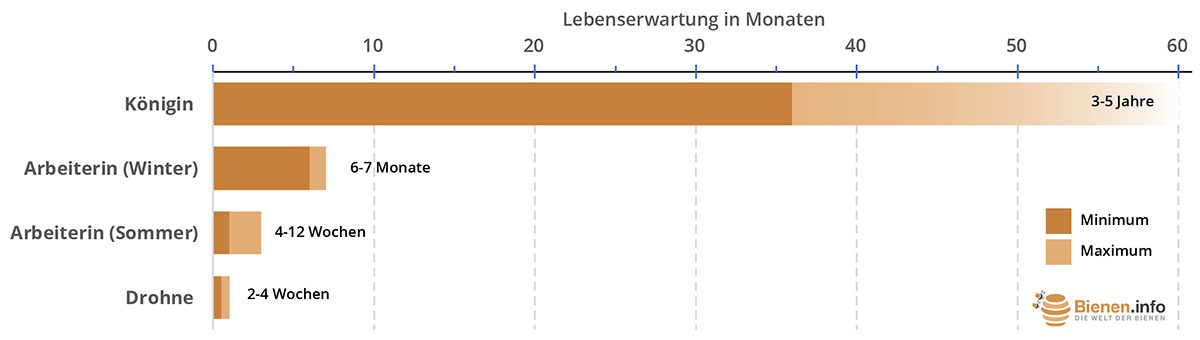
\includegraphics[width=400px]{0.bilder/lifeexpectancy.png}
    \end{center}
    \caption{Die minimale und maximale Lebenserwartung einer Biene jeder Kaste (\cite[]{bees:lifeexpectancy})} \label{image:lifeexpectancy}
\end{figure}

\subsubsection{Winter}
Die Vorbereitung auf den kommenden Winter beginnt bereits im Spätsommer, wobei neue Brut erzeugt wird für den Zweck der Überwinterung, sogenannte \textit{Winterbienen}. Ab Oktober werden die \textit{Sommerbienen} aus der Kolonie entfernt, sodass die Kolonie lediglich aus Winterbienen besteht. Dadurch, dass keine Energie für Brutpflege oder Sammelflüge aufgewendet werden muss, ist die Lebenserwartung der Winterbienen deutlich höher als die der Sommerbienen, wie bereits zuvor erläutert. Außerdem legen sich die Winterbienen ein Fettpolster zu, durch hohen Konsum von Pollen. Statt eines Winterschlafes formiert sich der Stock zu einer \textit{Wintertraube}, bei welcher die Kolonie die Königin umschließt und durch Muskelvibration warm hält. Mit Anfang des Frühlings wird mit gleicher Technik der Stock auf 35°C erhitzt, wodurch der Nahrungsverbrauch stark ansteigt aber das erfolgreiche Brüten der neuen Generation sichert. Sobald die ersten Blumen wieder sprießen setzen wieder die Sammelflüge ein \cite*[]{bees:winter}.
\subsection{Spiel-Engine}
Ein Videospiel wird heutzutage nicht mehr von Grund auf neu programmiert. Die Grundlage schafft in den meisten Fällen eine sogenannte \textit{Game Engine} (Spiele-Engine). Diese Engine bietet wichtige Grundlagen, welche es dem Entwickler oder dem Entwicklerteam deutlich vereinfachen loszulegen. Darunter fallen Grafik-, Physik- und Audiosysteme, welche je nach Engine variieren. Im Folgenden werden die drei größten Marktführer untersucht, verglichen und es wird anschließend in einem Fazit eine Entscheidung für eine dieser gefällt, welche für die Entwicklung des Prototypen verwendet wird.

\subsubsection{Godot}

\subsubsection{Unreal Engine}

\subsubsection{Unity}
\subsection{Spielwelt}
Die grundlegende Idee der Spielwelt ist, dass diese in zwei Instanzen geteilt wird. Die erste Instanz stellt die Oberwelt dar, wo Pflanzen und Bäume wachsen, wobei die zweite Instanz den Innenraum des Bienenstocks darstellt. In dem Bienenstock können Strukturen gebaut werden, welche in der Außenwelt nicht verfügbar sind. In der Außenwelt hingegen finden sich die Ressourcen, welche für das Fortleben essenziell sind. Für die gesamte Welt, in welcher das Spiel gespielt wird, stehen mehrere Optionen der Erstellung zur Verfügung.

\paragraph{Gridless}
Die erste Möglichkeit einer Spielwelt ist eine Karte ohne dargestelltes oder vorhandenes Grid. Solch ein System verwendet beispielsweise \textit{Age of Mythology}, wobei die Karte nicht in ein Grid, sondern viele tausende  Koordinaten eingeteilt ist. Diese Form der Positionierung ist daher gängig für \textit{Real Time Strategy} Spiele.

\paragraph{Square Grid}
Eine weitere Möglichkeit zur Positionierung von Gebäuden oder Einheiten innerhalb einer Spielwelt ist ein \textit{Square Grid} (vgl. \autoref{image:squaregrid}), also die Einteilung der Karte in eine gewisse Anzahl von Quadraten, welche als eigene Felder agieren und worauf Gebäude oder Einheiten zugreifen können. Dieses System wird unter anderem in \textit{Starcraft II} oder \textit{Age of Empires} verwendet, wodurch auch diese Form der Positionierung gängig für \textit{Real Time Strategy} ist. Allerdings findet man diese Eigenschaft auch in \textit{Turn Based Strategy}, darunter die älteren Teile der \textit{Civilization}-Reihe. Dieses System wurde im Laufe der Jahre jedoch von einem Square Grid auf ein Hex Grid umgestellt.

\begin{figure}
    \begin{center}
        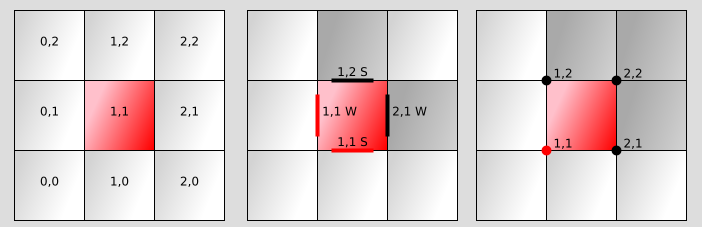
\includegraphics[width=300px]{0.bilder/squaregrid.png}
    \end{center}
    \caption{Aufbau eines Square Grids (\cite{world:grids})} \label{image:squaregrid}
\end{figure}

\paragraph{Hex Grid}
Die letzte Möglichkeit ist ein \textit{Hex Grid}, welches vor allem Anklang findet im Genre der \textit{Turn Based Strategy} Games, darunter \textit{Endless Legend}, \textit{Civilization VI} und \textit{Humankind}. Der klare Vorteil von einem Grid bestehend aus Hexagonen ist die \textit{Distanzberechnung} und die Anzahl \textit{direkter Nachbarn}. Im Vergleich zu einem Quadrat besitzt ein Hexagon in einem Grid 6 statt 4 direkter Nachbarn, wobei direkt bedeutet, dass die Kanten aneinander angrenzen. Um einen diagonalen Weg in einem Square Grid einzuschlagen, muss ein weiterer Weg aufgewendet werden, da nach dem \textit{Satz des Pythagoras} gilt:
\begin{equation}
    a^2 + b^2 = c^2
\end{equation}
Der diagonale Weg innerhalb eines Quadrates mit Länge 1 und Breite 1 wäre folglich 
\begin{equation}
    \sqrt{1^2 + 1^2} = \sqrt{2}
\end{equation}
Wobei offensichtlich gilt, dass
\begin{equation}
    \sqrt{2} > 1
\end{equation}
Möchte man also Bewegungen von Einheiten in 6 statt 4 Richtungen ermöglichen, empfiehlt sich ein Hex Grid statt einem Square Grid. Die Distanz zwischen allen gegenüberliegenden Kanten eines Hexagons ist stets gleichlang (vgl. \autoref{image:hexgrid}). Unter der Berücksichtigung, dass die Thematik der Bienen auch mit \textit{Bienenwaben} und deren hexagonalen Form assoziiert wird, wird der Prototyp ein Hex Grid verwenden. 
\begin{figure}
    \begin{center}
        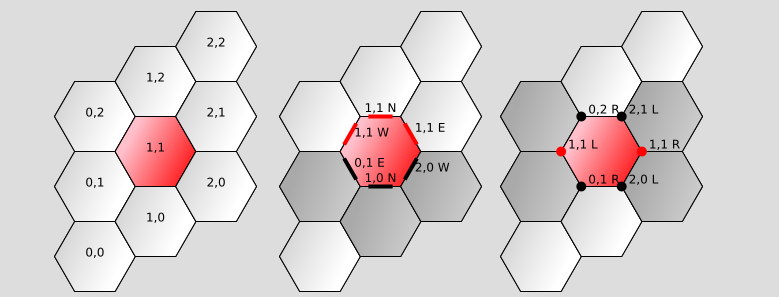
\includegraphics[width=300px]{0.bilder/hexgrid.png}
    \end{center}
    \caption{Aufbau eines Hex Grids (\cite{world:grids})} \label{image:hexgrid}
\end{figure}

\subsubsection{Generierung}
Das Terrain beziehungsweise Grid wird über einen vielschichtigen Algorithmus generiert, welcher die gesamte Fläche in Columns und die Columns wiederum in Chunks unterteilt. Der Algorithmus wurde mittels eines im Internet gefundenen Tutorials \cite*[]{world:tutorial} erarbeitet und anschließend angepasst. Mittels der Methode \textit{GenerateMap} (vgl. \autoref{code:worldgeneration}) kann von außerhalb dann der Algorithmus verwendet werden. Es gibt etliche Variationen zur Anpassung, darunter ein Seed, welcher die Generierung beeinflusst, Meeresspiegel, Erosion, Feuchtigkeit und Temperatur, es ist damit viel Diversität zwischen verschiedener Karten gegeben. In dieser Arbeit wird nicht weiter auf dieses Tutorial eingegangen, ist jedoch für weitere Informationen verlinkt. Der Bienenstock ist in dem Prototypen lediglich eine kleinere Version der generierten Außenwelt und noch nicht visuell als Bienenstock erkennbar. Dies wird in zukünftigen Iterationen angepasst und gelb und orange eingefärbt. Außerdem soll ein Ausgang für die Bienen in dem Bienenstock generiert werden, durch welchen die Einheiten sich von Bienenstock nach Außenwelt und umgekehrt bewegen können. 

\definecolor{LightGray}{gray}{0.9}
\begin{listing}[H]
\caption{World Generation}
\label{code:worldgeneration}
\begin{minted}[
bgcolor=LightGray,
framesep=2mm,
baselinestretch=1.2,
fontsize=\footnotesize,
linenos,
]{csharp}
public void GenerateMap (int x, int z, bool wrapping) {
    Random.State originalRandomState = Random.state;
    if (!useFixedSeed) {
        seed = Random.Range(0, int.MaxValue);
        seed ^= (int)System.DateTime.Now.Ticks;
        seed ^= (int)Time.unscaledTime;
        seed &= int.MaxValue;
    }
    Random.InitState(seed);

    cellCount = x * z;
    overworldGrid.CreateMap(x, z, wrapping);
    if (searchFrontier == null) {
        searchFrontier = new HexCellPriorityQueue();
    }
    for (int i = 0; i < cellCount; i++) {
        overworldGrid.GetCell(i).WaterLevel = waterLevel;
    }
    CreateRegions();
    CreateLand();
    ErodeLand();
    CreateClimate();
    CreateRivers();
    SetTerrainType();
    for (int i = 0; i < cellCount; i++) {
        overworldGrid.GetCell(i).SearchPhase = 0;
        overworldGrid.GetCell(i).MapType = HexMapType.Overworld;
    }

    Random.state = originalRandomState;
}
\end{minted}
\end{listing}
\subsection{Spielbeginn}
Das Spiel beginnt auf der nun zufällig generierten, hexagonalen Spielwelt. Es wird mit exakt zwei \textit{Arbeitsbienen} und einer \textit{Königin} gestartet, welche sich im mittleren Alter befinden. Diese Bienen starten auf drei zufälligen Kacheln nebeneinander auf einer zufällig generierten Karte.

\subsection{Gameplay Loop}
Der primäre \textit{Gameplay Loop} besteht darin, die Bienenkolonie am Leben zu halten. Nach Spielbeginn wird der Spieler mit den gegebenen Arbeitsbienen und der Königin auf sich alleine gestellt. Der Spieler sollte damit anfangen, etwas Nektar und Pollen zu sammeln, um diese dann zu Bienenwachs zu verarbeiten und einen Stock zu bauen. Innerhalb dieses Stocks sollte die Königin beginnen, Drohnen heranzuziehen, mit welchen man wiederum neue Arbeiterinnen und/oder eine neue Königin heranziehen kann. Das Ziel besteht darin, das Überleben der Kolonie möglichst lange zu sichern. Die Herausforderung besteht darin, dass die Winter schwer sind und mit der Zeit auch immer schwerer werden. Es gilt, die Balance zu finden zwischen Nahrungsbeschaffung, Erweiterung des Stocks und Erzeugung neuer Brut. Zeugt der Spieler zu viel neue Bienen, kippt das Gleichgewicht und die Kolonie stirbt an einem Mangel an Nahrung. Das grobe Konzept des Gameplay Loops ist in \autoref{image:gameplayloop} veranschaulicht.

\begin{figure}
    \begin{center}
        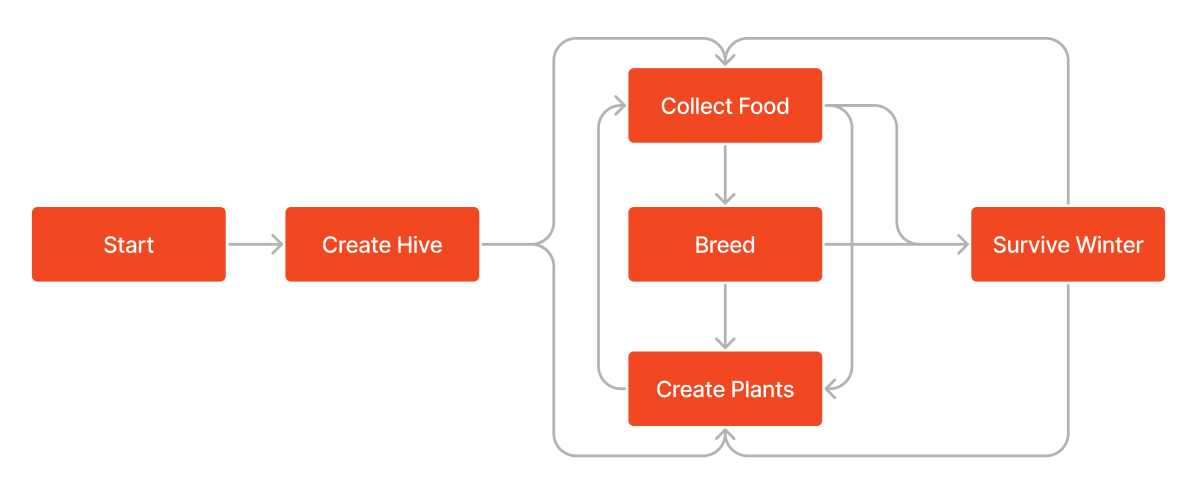
\includegraphics[width=300px]{0.bilder/gameplayloop.PNG}
    \end{center}
    \caption{Grobe Skizze des Gameplay Loops} \label{image:gameplayloop}
\end{figure}
\subsection{Spielende}
Analog zu \textit{SimCity 2000} gibt es kein direkt vordefiniertes Ende. Der Endzustand des Game Over wird jedoch erreicht, wenn keine Königin mehr verfügbar ist, um die Kolonie zu leiten. Das Spiel ist also theoretisch unendlich lange spielbar, sollte jedoch von der Schwierigkeit so gesteigert werden, dass ein natürliches Ende nach einiger Zeit eintritt. Die Endzustände des Spieles können später noch angepasst werden, eine Idee wäre es, dem Spieler nach Sterben der Königin noch etwas mehr Zeit zu geben um darauf reagieren zu können, sodass eine gerade herangezogene Königin noch die Chance hat zu schlüpfen. Es könnte auch die maximale Jahreszahl begrenzt werden und dem Spieler eine Siegbedingung bereitstellen, in Form eines Überlebens für eine gewisse Zeit.

\subsection{Mechaniken}
Es wurden nun in \textit{Sektion 2} und \textit{Sektion 3} einige Mechaniken und Eigenheiten von älteren und neu erschienen Management Games untersucht und Hypothesen dazu angeführt. Diese Hypothesen und Mechaniken, welche sich als besonders interessant und nutzerfreundlich erweisen, werden nun unter Berücksichtigung der in \textit{Sektion 4.1} erörterten Vorgänge innerhalb einer Bienenkolonie konkretisiert und ausgefeilt. Außerdem werden die in \textit{Sektion 1} definierten Eigenschaften eines Resource Management Games berücksichtigt und versucht, die untersuchten Gegebenheiten (Ressourcen, Ökonomie, Informationsgehalt und Verwaltungsaspekte) möglichst sinnvoll mit den Vorgängen einer Bienenkolonie zu kombinieren, um daraus ein Spiel zu gestalten, welches sehr stark an die echten Vorgänge einer solchen angelehnt ist. Im folgende referenzierte Hypothesen aus \autoref{table:hypotheses} werden mit [HX] abgekürzt, wobei X für die jeweilige Nummer der Hypothese steht.

\subsubsection{Anweisungsstil}
Wie sich in den Interviews und der Analyse von RimWorld gezeigt hat, lassen sich die Art, auf welche Anweisungen an die jeweiligen Einheiten erteilt werden, in \textit{direktes} und \textit{indirektes} Anweisen beziehungsweise Zuweisen. Während in den bereits vorgestellten Titeln meistens auf eine direkte Anweisung der Einheiten zurückgegriffen wird, stellt RimWorld eine Neuerung dar, welche laut [H15] für das Genre des Colony Managements als durchaus positiv von den Probanden aufgefasst wird. Daher wird dieser Anweisungsstil, mitsamt der Prioritätenliste [H13], welche mittels Grafiken verständlicher gemacht wird [H14]. Diese Grafiken finden sich in \autoref{image:prioritylist} wieder. Es gibt fünf verschiedene Prioritätszustände pro Tätigkeitsbereich pro Biene. Falls die Biene aufgrund ihrer Kaste oder ihres Alters eine bestimmte Tätigkeit nicht machen kann, ist der Button nicht vorhanden. Ansonsten gilt, dass ein grüner Pfeil nach oben bedeutet \textit{Hohe Priorität}, ein gelber Strich bedeutet \textit{Mittlere Priorität}, ein roter Pfeil nach unten bedeutet \textit{Niedrige Priorität}. Falls keine Grafik in dem Button angezeigt wird, steht dies für \textit{Untätig}, womit der Spieler auch entscheiden kann, dass manche Bienen bestimmte Tätigkeiten nicht erledigen, selbst wenn möglich. Wird eine Aktion auf ein Feld angewiesen, wird eine \textit{JobOrder} erstellt, welche alle wichtigen Informationen enthält (vgl. \autoref{code:addjoborder}). Diese JobOrder wird in eine Liste hinzugefügt, welche jedes Frame iteriert wird, und geschaut, ob noch offene Anfragen vorhanden sind. Für jede offene Anfrage wird anhand einer Liste vieler Kriterien eine Biene aus der Liste aller vorhandenen adulten Bienen gesucht (vgl. \autoref{code:assignjobs}). Zuerst werden alle Bienen gesucht, welche keine Anfrage zugewiesen haben, theoretisch die Anfrage ausführen können und ausgewachsen sind. In einer zweiten Iteration werden die nun ausgesuchten Bienen auf Prioritäten geprüft, die Bienen mit der jeweils höchsten Priorität werden in einer Liste gespeichert. Zuletzt werden spezifische Informationen gesucht, wie etwa ein passendes Inventar für die Anfrage, beispielsweise genug Pollen für die Anfrage Pollinate. Letztendlich sollte von dieser dritten Liste die Biene mit dem kürzesten Pfad ausgewählt werden, wobei dieser letzte Schritt aus zeitlichen Gründen noch nicht im Prototyp vorhanden, aber algorithmisch durchaus möglich ist.

\begin{figure}
    \begin{center}
        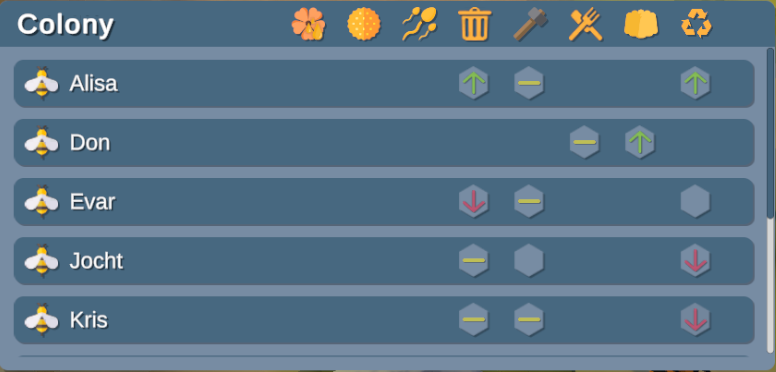
\includegraphics[width=300px]{0.bilder/prioritylist.png}
    \end{center}
    \caption{Fertig implementierte Prioritätenliste} \label{image:prioritylist}
\end{figure}

\definecolor{LightGray}{gray}{0.9}
\begin{listing}[H]
\caption{Erstellung einer neuen Anweisung}
\label{code:addjoborder}
\begin{minted}[
bgcolor=LightGray,
framesep=2mm,
baselinestretch=1.2,
fontsize=\footnotesize,
linenos,
]{csharp}
public JobOrder AddJobOrder(Bee bee, BeeAction action, HexCell hexCell) {
    JobOrder jobOrder = new JobOrder();
    jobOrder.Action = action;
    jobOrder.AssignedBee = bee;
    jobOrder.Finished = false;
    jobOrder.MapType = hexCell.MapType;
    jobOrder.Cell = hexCell;
    
    jobQueue.Add(jobOrder);
    hexCell.AssignJob(jobOrder);
    hexCell.ShowJobHighlight();
    return jobOrder;
}
\end{minted}
\end{listing}

\definecolor{LightGray}{gray}{0.9}
\begin{listing}[H]
\caption{Zuweisung einer Biene von einer offenen Anweisung}
\label{code:assignjobs}
\begin{minted}[
bgcolor=LightGray,
framesep=2mm,
baselinestretch=1.2,
fontsize=\footnotesize,
linenos,
]{csharp}
private void AssignJobs() {
    for (int i = 0; i < jobQueue.Count; i++) {
        JobOrder jobOrder = jobQueue[i];
        Bee bee = jobOrder.AssignedBee == null ? 
        FindBee(jobOrder) : jobOrder.AssignedBee;
        if (bee) {
            jobOrder.AssignedBee = bee;
            bee.AssignJob(jobOrder);
            this.activeJobs.Add(jobOrder);
            this.jobQueue.Remove(jobOrder);
            bee.Travel(jobOrder.Cell);
        }
    }
}
\end{minted}
\end{listing}

\subsubsection{Ressourcen}
Die im Spiel vorhandenen Ressourcen sind in \autoref{table:resources} aufgelistet. Die Gründe für die Auswahl der Ressourcen sind \textit{Sektion 4.1.1} zu finden. \textit{Honigtau} wird nicht als Ressource implementiert, da diese von lebenden Tieren extrahiert wird, und aufgrund von weiteren benötigten Modellen und Animationen keine weiteren Tiere neben den eigentlichen Bienen implementiert werden. Um das Spiel spannender und etwas komplexer zu gestalten werden verschiedene \textit{Sources}, \textit{Converter} und \textit{Drains} (vgl. \textit{Sektion 1.1.2}) verwendet. Alle involvierten Ressourcen, wie auch baubare Waben, sind in \autoref{image:resourceloop} skizziert. Die Zahlen sind dabei rein experimentell und müssen im Verlauf der Tests gegebenenfalls angepasst werden.

\begin{table}[]
    \centering
    \caption{Verfügbare konkrete Ressourcen}
    \label{table:resources}
    \begin{tabular}{|l|l|}
    \hline
    Nahrung     & Nektar, Honig, Pollen, Royal Jelly, Wasser \\ \hline
    Baumaterial & Bienenwachs                                \\ \hline
    Einheiten   & Königinnen, Drohnen, Arbeitsbienen         \\ \hline
    \end{tabular}
\end{table}

\paragraph{Nektar}
Nektar wird ausschließlich von Blumen extrahiert, welche eine \textit{Source} darstellen. Jedoch ist an jede Blume eine Bedingung geknüpft. Blumen haben ein eigenes Inventar für Nektar und Pollen, welches bei Extraktion durch eine Biene geleert wird und neu regenerieren muss. Eine Biene sollte also frequentiv die Blumen wechseln, um möglichst viele Ressourcen zu sammeln. Nektar hat eine gewisse Lebensdauer und wird nach einiger Zeit schlecht, wodurch eine gewisse Anzahl von Nektar aus dem Spiel entfernt wird. Diese Lebensdauer agiert dadurch als \textit{Drain}.

\paragraph{Pollen}
Die zweite Ressource sind die Pollen, welche ebenfalls von Blumen extrahiert werden. Pollen können unter anderem verwendet werden, um neue Blumen zu pflanzen und spielen daher gerade im Frühling eine große Rolle, aber auch für das Herstellen für Bienenwachs und Gelée Royal. Pollen besitzen eine etwas längere Lebensdauer und können daher über den Winter gelagert werden. Dadurch, dass Pollen mehrere Anwendungsfälle besitzen, muss der Spieler abwägen, für welchen er diese Ressource am ehesten verwendet beziehungsweise wie er die vorhandenen Ressourcen aufteilt.

\paragraph{Honig}
Honig ist eine manuell hergestellte Ressource, welche an einem \textit{Evaporator}, also einer leicht umgebauten Wabe, von einer Biene hergestellt werden kann. Dieser Evaporator stellt, neben den anderen baubaren Waben, einen \textit{Converter} dar. Ein wichtiger Aspekt des Honigs ist der Fakt, dass man mehr als ein Nektar pro Honig verwenden muss, damit der Spieler abwägen muss, ob es die Herstellung wert ist. Dadurch entsteht mehr Komplexität und der Spieler besitzt Entscheidungsfreiheit. So könnten manche Spieler versuchen, lediglich genug Honig für den Winter herzustellen, und andere wiederum jeglichen Nektar direkt in Honig umwandeln. Es entsteht somit eine mögliche \textit{Strategie}.

\paragraph{Bienenwachs}
Entgegen der anderen Ressourcen ist Bienenwachs keine Nahrung. Diese Ressource wird einzig und allein für den Bau neuer Strukturen verwendet. Diese Strukturen werden im Folgenden näher erläutert. Bienenwachs muss an einem \textit{Mixer} hergestellt werden, welcher sowohl Honig als auch Pollen verwendet, um neues Bienenwachs herzustellen. Aus diesem Bienenwachs können dann \textit{Brutwaben, Lagerwaben} und \textit{Refiner} hergestellt werden, wie auch ein neuer Stock, sollte man den gegebenen verlagern wollen.

\paragraph{Gelée Royal}
Eine weitere fundamentale Ressource ist das Gelée Royal oder auch \textit{Royal Jelly}, welches an einem \textit{Refiner} durch Vermischen von Pollen und Honig erzeugt werden kann. Diese Ressource ist wichtig für das Heranziehen einer neuen Königin und wird in die Brutwabe einer \textit{Arbeitsbienenlarve} gegeben, damit diese sich zu einer Königin entwickelt.

\paragraph{Wasser}
Die einzige nicht vom Spieler sammelbare oder lagerbare Ressource ist Wasser. Dieses müssen die Bienen durch Nahrung aufnehmen (Nektar besitzt mehr Wasser als Honig), oder über das Trinken an einem Fluss. Da im Winter keine Ausflüge gestattet sind, ist es wichtig, dass Bienen vor dem Winter genug Wasser zu sich nehmen, um nicht zu verdursten.

\paragraph{Königin, Drohne und Arbeitsbiene}
Diese greifbaren Ressourcen sind das Fundament des Spiels, wobei neue Bienen, analog zu \textit{Sektion 4.1.3}, Kasten-spezifisch herangezogen werden können, mehr dazu im folgenden Abschnitt.

\begin{figure}
    \begin{center}
        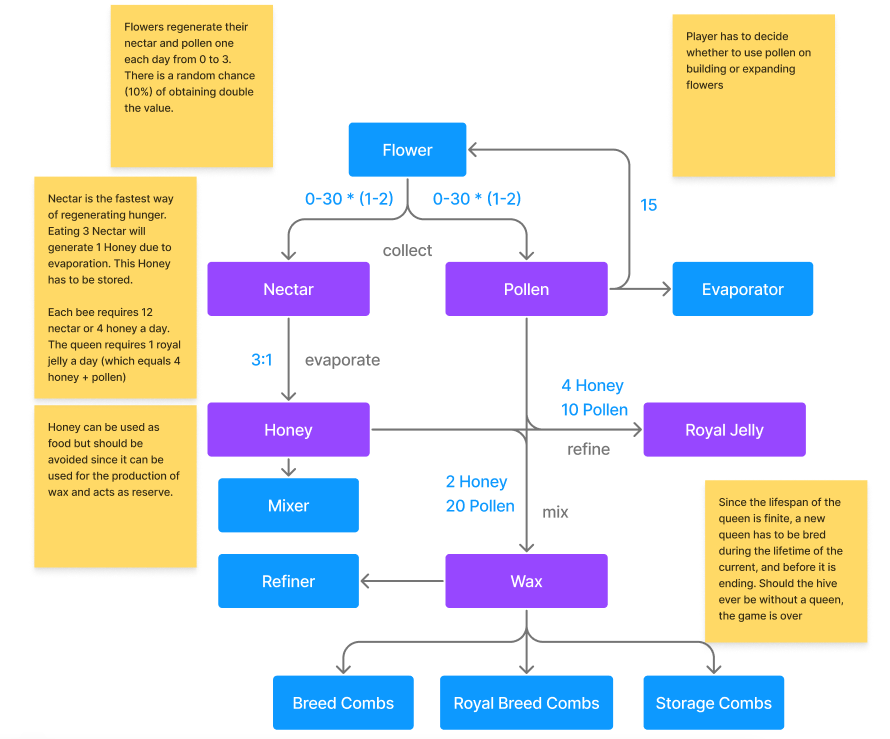
\includegraphics[width=300px]{0.bilder/resourceloop.png}
    \end{center}
    \caption{Ressourcenverlauf und mögliche Umwandlungen} \label{image:resourceloop}
\end{figure}

\subsubsection{Jahreszeiten}
Es gibt vier verschiedene Jahreszeiten, \textit{Frühling, Sommer, Herbst} und \textit{Winter}. Alle 30 Tage wechselt die Jahreszeit zur jeweils nächsten. Jede Jahreszeit ist dabei anders und bietet andere, mögliche Events. Jegliche Angaben von Chancen sind dabei rein experimentell und müssen im späteren Verlauf getestet werden. Im Prototypen werden aufgrund der niedrigen Zeitspanne keine Events implementiert sein, jedoch bereits konzipiert für die spätere Implementation.

\paragraph{Frühling} ist die Zeit, in welcher neue Blumen sprießen. Es gibt ein besonderes Event namens \textit{Pollenflug}, wobei besonders viele Blumen sprießen, was es dem Spieler durchaus erleichtern kann, neue Nahrung zu beschaffen. Das Event hat eine Chance von $\frac{1}{30}$ pro Tag zu passieren, und kann pro Jahr maximal ein Mal geschehen.

\paragraph{Sommer} ist die Zeit der Hitze und des \textit{Schwärmens}. Deshalb gibt es zwei Events welche passieren können, das erste ist die \textit{Dürre}, wobei einige Blumen sterben und manche Flüsse austrocknen. Die Chance dafür ist pro Tag $\frac{1}{60}$. Das zweite ist das Schwärmen, welches jedes Jahr erneut passiert, insofern eine Königin vorhanden ist. Dabei wird angegeben, dass die Königin den Stock verlassen wird. Deshalb ist der Spieler dazu gezwungen, eine neue Königin heranzuziehen, da ansonsten keine Königin mehr vorhanden sein wird. Die Königin wird dabei einen kleinen Anteil der Kolonie mitnehmen (mindestens eine \textit{Arbeitsbiene} und \textit{20\%} der Arbeitsbienen). Diese Zahl ist variabel und wird gegebenenfalls angepasst. Der Spieler wird also etwas zurückgesetzt und gezwungen, zu handeln, was die Herausforderung durchaus erschwert. 

\paragraph{Herbst} bringt zwei negative Events mit sich. Es kann jeden Tag mit einer $\frac{1}{60}$ Chance passieren, dass jegliche Blumen weniger Ertrag geben in entweder Pollen oder Nektar. Auch hier wird der Spieler dazu gezwungen, sich anzupassen und sinnvoll darauf zu reagieren. Zudem ist die Chance auf Regen durchaus etwas höher, als sonst in den Jahreszeiten. Als wiederkehrendes Event, analog zum Schwärmen, steht jedes Jahr der \textit{Drohnenkrieg} beziehungsweise die \textit{Drohnenschlacht} an, wobei sämtliche Drohnen aus dem Stock 

\paragraph{Winter} ist die Zeit des Notstands. Die Bienen sind in dieser Zeit nicht ausflugfähig und müssen in ihrem Bienenstock warten, bis der Winter endet. Daher muss darauf geachtet werden, dass genug Honig gelagert ist, damit die Kolonie überleben kann. Sollte Regen während dieser Zeit fallen, ist dieser stattdessen Schnee. Es sterben zu dieser Jahreszeit sämtliche Blumen ab, wodurch, selbst wenn eine Biene rausfliegen würde, es keine Möglichkeit gibt, Nahrung zu beschaffen.


\begin{figure}
    \begin{center}
        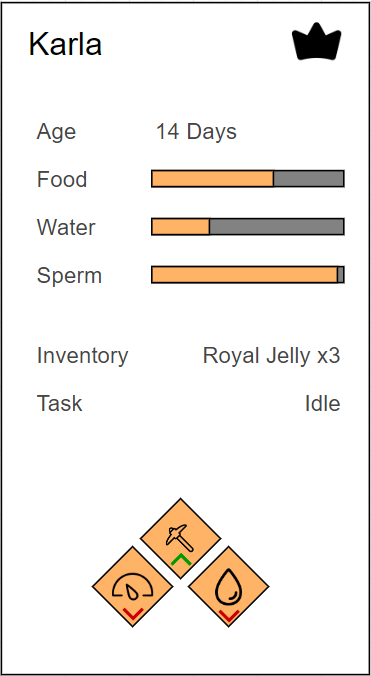
\includegraphics[width=100px]{0.bilder/beeinfodraw.PNG}
    \end{center}
    \caption{Skizze des Informationsfensters einer ausgewählten Biene} \label{image:beeinfodraw}
\end{figure}

\subsubsection{Bienen}
Die Bienen sind das Herzstück des Spiels und werden analog zu \textit{RimWorld} indirekt gesteuert. Eine Biene hat mehrere Eigenschaften. Sämtliche aufgelisteten Eigenschaften sind visuell dargestellt als Skizze beziehungsweise Mockup in \autoref{image:beeinfodraw}.

\paragraph{Kasten}
Es gibt analog zu einer realen Bienenkolonie drei verschiedene Kasten. Jede Biene besitzt eine Variable in Form einer Enum, welche angibt, ob es sich um eine Königin, eine Drohne oder eine Arbeitsbiene handelt. Aufgrund dieser Information werden etliche Entscheidungen getroffen, darunter das gezeigte Modell, wovon es drei verschiedene für jede Kaste gibt, die möglichen ausführbaren Aktionen und die Lebensdauer. Es können kastenspezifisch neue Bienen herangezogen werden. Wie auch in der realen Welt werden für die Arbeitsbienen befruchtete Eier benötigt, für die Königinnen befruchtete Eier und Royal Jelly, und für die Drohnen lediglich unbefruchtete Eier. Diese Mechanik ist in \autoref{image:reproductionloop} schematisch dargestellt.

\begin{figure}
    \begin{center}
        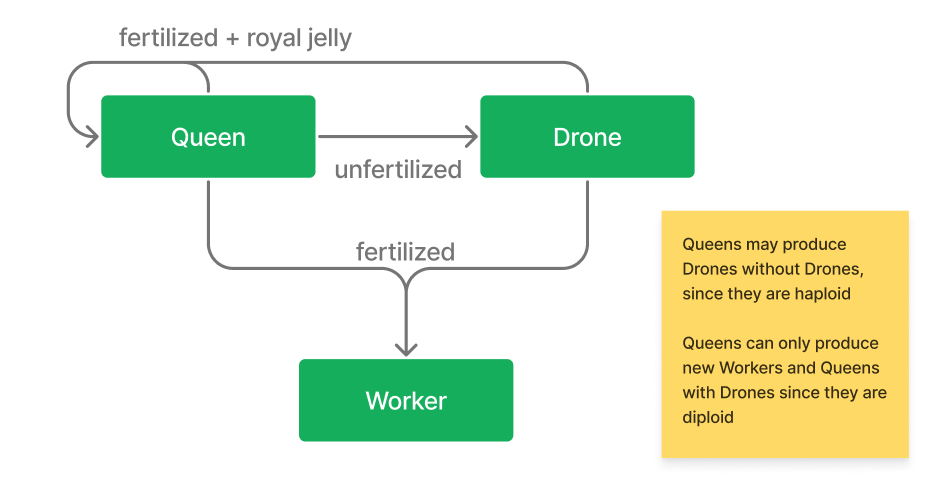
\includegraphics[width=300px]{0.bilder/reproductionloop.png}
    \end{center}
    \caption{Reproduktionsverhalten der Bienen} \label{image:reproductionloop}
\end{figure}

\paragraph{Name}
Jede Biene hat zur besseren Unterscheidung einen zufällig generierten Namen aus einer großen Variation verschiedenster Ethnien. Der Generator entstammt dem Unity Asset Store \cite*[]{asset:namegenerator}.

\paragraph{Alter} 
Das Alter der Biene ist von zentraler Bedeutung. Für die Königin ist es entscheidend einzuschätzen, wie lange diese noch lebt, für die Arbeitsbienen ist es wichtig zu erkennen, welche Arbeiten und Aufgaben diese übernehmen kann. Eine Biene am Ende ihres Lebens ist biologisch nicht mehr in der Lage, die neue Brut zu füttern, und dient lediglich dem Sammeln von Ressourcen.

\paragraph{Hunger} 
Eine Biene hat das Bedürfnis nach Nahrung. Der Nahrungsbalken wird mit der Zeit weniger, weshalb die Biene Nahrung beschaffen muss, jedoch nicht aktiv. Ist Nahrung vorhanden und die Biene erreicht einen Schwellenwert, wird sich diese Biene die Nahrung eigenständig aus dem Lager entnehmen. Ist der Wert der Nahrung zu lange auf 0, stirbt die Biene. Die voreingestellte Reihenfolge der verspeisten Nahrung lautet:

\begin{center}
    Nektar > Honig > Pollen
\end{center} Royal Jelly wird nicht von den Arbeitern angerührt und wird lediglich von der Königin verspeist, genau so wie für das Heranziehen neuer Königinnen zur Larve gegeben. Stetige Bewegung sorgt für schnelleren Hunger. Die Reihenfolge der Nahrung kann vom Spieler angepasst werden, wodurch mehr Entscheidungsfreiheit gegeben ist und mehr Taktik angewandt werden kann. So könnte ein Spieler möglichst viele Pollen sammeln und diese als primäre Nahrungsquelle nutzen. Natürlich müssen diese Mechaniken ausgiebig getestet werden, sodass verschiedene Strategien nicht zu unausgeglichen sind. Diese Änderung, wie auch das Futtern oder Füttern, ist im gegebenen Prototypen nicht implementiert.

\paragraph{Durst} 
Bienen benötigen Flüssigkeit, genauer gesagt Wasser. Dieses wird nicht im Stock gelagert, sondern an Flüssen getrunken. Je mehr sich eine Biene bewegt, desto mehr Flüssigkeit benötigt diese. Sinkt dieser Wert auf 0, wird die Biene nach kurzer Zeit sterben. Die Funktionalität des Trinkens ist im Prototypen noch nicht implementiert, jedoch stirbt eine Biene an Durst, sobald der gegebene Wert auf 0 sinkt.

\paragraph{Samen} 
Diese Eigenschaft hat lediglich eine Königin, und gibt an, wie viel Samen der Drohnen noch vorhanden sind um neue und befruchtete Eier zu legen. Es ist wichtig darauf ein Auge zu haben, da ohne verfügbare Samen weder Arbeitsbienen, noch Königinnen herangezogen werden können. Die Aktion zieht aus dem Pool der vorhandenen in der Königin gespeicherten Samen einen Wert ab, sodass die Anzahl der Aktion durch diese nicht greifbare Ressource limitiert ist.

\paragraph{Inventar} 
Das Inventar besitzt jede Biene und zeigt an, was diese gerade trägt. Getragen werden können Nektar, Pollen, Honig, Royal Jelly und Bienenwachs. Die Menge richtet sich nach der Art des Getragenen. Das Inventar ist ein zentraler Punkt der Ressourcen, da Bienen für Aktionen in den meisten Fällen die benötigte Ressource erst aus dem Lager holen müssen, falls nicht bereits im Inventar vorhanden, und dann diese nicht greifbaren Ressourcen weiterverwenden mittels Converter.

\paragraph{Auftrag} 
Der momentane Auftrag ist ebenfalls Teil der Biene. Dieser zeigt dem Nutzer, was diese Biene gerade vorhat und wieso sie sich zu der bestimmten Stelle bewegt.

\paragraph{Genetische Eigenschaften / Traits} 
Die genetischen Eigenschaften beziehungsweise \textit{Traits} sind immer exakt drei Stück und werden nach [H6] in überschaubarer Anzahl gehalten und so benannt, dass aus dem Namen der Effekt grundlegend ersichtlich ist. Diese können sowohl \textit{positive} als auch \textit{negative} Auswirkungen auf die Effizienz der einzelnen Biene haben, wobei nicht eindeutig erkennbar sein soll, welcher der effektiv beste oder schlechteste Trait ist, der zur Auswahl steht, um [H7] nachzugehen, und Nutzer-eigene Strategien zu fördern. Die möglichen Traits und ihre Wahrscheinlichkeiten sind in \autoref{table:traits} zu finden. Die Traits sind vererbbar, wobei bei der Vererbung eine Chance besteht, dass ein Trait \textit{mutiert} und deshalb in einen anderen, zufälligen, geändert wird. Wird eine Königin von mehreren verschiedenen Drohnen besamt, werden die Erbinformationen gespeichert. Ob der jeweilige Trait nun von der Seite des Vaters oder der Seite der Mutter übernommen wird, ist gleichverteilt 50:50. Seien die besamenden Drohnen folgende:

\begin{itemize}
    \item Drohne A: Schillernd, Arbeitsfreudig, Gesegnet
    \item Drohne B: Schillernd, Arbeitsfreudig, Verflucht
    \item Drohne C: Schillernd, Großer Magen, Verdampfer
\end{itemize} Und die Königin besäße folgende Eigenschaften:

\begin{itemize}
    \item Königin: Schillernd, Großer Magen, Empfänglich
\end{itemize} Dann gelten folgende Chancen für die Traits der Brut:

\begin{itemize}
    \item Schillernd: $100\%$
    \item Empfänglich: $\frac{1}{2}$
    \item Großer Magen: $\frac{1}{3} + \frac{1}{2} = \frac{5}{6}$
    \item Arbeitsfreudig: $\frac{2}{3} \times \frac{1}{2} = \frac{1}{3}$
    \item Gesegnet: $\frac{1}{3} \times \frac{1}{2} = \frac{1}{6}$
    \item Verflucht: $\frac{1}{3} \times \frac{1}{2} = \frac{1}{6}$
    \item Verdampfer: $\frac{1}{3} \times \frac{1}{2} = \frac{1}{6}$
\end{itemize} Die Traits, welche speziell auf eine gewisse Art von Kaste gelten, werden im Hintergrund gespeichert und es wird ein neuer Trait gezogen. Dieser wird sich vorgemerkt. Sollte die Arbeitsbienenlarve also zur Königin herangezogen werden, wird der vorgemerkte Trait durch den Erstgezogenen ersetzt. Die Traits sind bereits namentlich implementiert, es werden drei bei der Geburt der Biene zugewiesen. Allerdings haben diese im Prototypen noch keine weiteren Effekte und keine passenden Grafiken. Auch werden die Traits noch nicht genetisch vererbt, sondern zufällig gezogen, was sich im Laufe der Entwicklung noch ändern wird.

\paragraph{Mutation}
Damit eine Diversität entstehen kann, und nicht stetig die gleichen Traits in der Kolonie weitervererbt werden, bedarf es der Möglichkeit einer Mutation. Es besteht eine geringe Chance, dass \textit{nach dem Ziehen} eines vererbten Traits, dieser Trait durch einen völlig anderen ersetzt wird. Diese Mechanik ist in dem Prototypen noch nicht gegeben.
% Please add the following required packages to your document preamble:
% \usepackage{graphicx}
\begin{table}[]
    \centering
    \caption{Mögliche Traits einer Biene}
    \label{table:traits}
    \resizebox{\columnwidth}{!}{%
    \begin{tabular}{|l|l|l|}
    \hline
    Arbeitsfreudig / Arbeitsscheu (Alle)        & Erledigt alle Aufgaben 10\% schneller / langsamer                                        & 12\% \\ \hline
    Sammelfreudig / Sammelscheu (Arbeitsbiene)  & Sammelt Ressourcen 15\% schneller / langsamer                                            & 12\% \\ \hline
    Fingerfertig / Grobmotorisch (Arbeitsbiene) & Stellt neue Ressourcen 10\% schneller / langsamer her.                                   & 12\% \\ \hline
    Sparsam / Freigiebig (Arbeitsbiene)         & Verbraucht beim Füttern etwas weniger / mehr Nahrung.                                    & 12\% \\ \hline
    Empfänglich / Unempfänglich (Königin)       & Benötigt weniger / mehr Drohnen um die Samen zu füllen und hat mehr / weniger Kapazität. & 12\% \\ \hline
    Gesegnet / Verflucht (Alle)                 & Lebt ein längeres / kürzeres Leben.                                                      & 12\% \\ \hline
    Wasserspeicher / Verdampfer (Alle)          & Benötigt weniger / mehr Wasser und verbraucht weniger / mehr.                            & 12\% \\ \hline
    Kleiner / Großer Magen (Alle)               & Benötigt weniger / mehr Nahrung und verbraucht weniger / mehr.                           & 12\% \\ \hline
    Königliche Immunität (Drone)                & Die Drohne ist ausgenommen von der Drohnenschlacht.                                      & 2\%  \\ \hline
    Schillernd (Alle)                           & Die Biene sieht anders aus als gewöhnliche Bienen.                                       & 2\%  \\ \hline
    \end{tabular}%
    }
    \end{table}



\subsubsection{Aktionen}
Es gibt 6 verschiedene, vom Spieler ausführbare, Anordnungen. Diese werden verwendet, um die Bienen indirekt zu steuern und den Stock somit möglichst am Leben zu erhalten. Von den Aktionen sind im Prototyp das Sammeln, das Bestäuben, das Eier legen und das Abbrechen funktional. 

\paragraph{Sammeln} wird verwendet, um von den in der Spielwelt vorhandenen Blumen den Nektar und die Pollen zu extrahieren. Diese Aktion ist lediglich von Arbeitsbienen im späten Alter ausführbar.

\paragraph{Bestäuben} verwendet Pollen, um neue Blumen zu erstellen, welche als weitere Quelle von Nektar und Pollen agieren. Dies kann sinnvoll sein, sollten nicht genug Blumen vorhanden sein, etwa im Frühling nach einem harten Winter. Diese Aktion ist ebenfalls nur von älteren Bienen ausführbar.

\paragraph{Besamen} ist eine Aktion, welche lediglich den Drohnen vorbehalten ist. Mit Auswahl der Königin finden sich nacheinander Drohnen, bis die Königin keine weiteren Samen speichern kann.

\paragraph{Eier legen} wird lediglich von der Königin ausgeführt. Nach Auswahl einer passenden Brutwabe (normale Brutwabe oder königliche Brutwabe), fliegt die Königin zu der jeweiligen Stelle und legt ein Ei ab. Ob dieses befruchtet ist oder nicht hängt davon ab, ob die Königin Samen gespeichert hat.

\paragraph{Abbrechen} wird verwendet, um eine bereits ausgeführte Anordnung zurückzuziehen. Anders als die anderen Aktionen ist hierfür keine Biene nötig.

\paragraph{Zerstören} kann verwendet werden, um vom Spieler gebaute Strukturen wieder zu vernichten. Diese Aktion ist lediglich von mittelalten Arbeitsbienen ausführbar und ist auf den Bienenstock beschränkt.

\subsubsection{Strukturen}
Es gibt, analog zu den Aktionen, 6 verschiedene, baubare Strukturen. Diese dienen in den meisten Fällen als \textit{Converter} und Arbeitsstätte der Bienen, aber auch als Lagerplatz. Sämtliche baubare Strukturen sind \autoref{image:resourceloop} zu entnehmen.

\paragraph{Evaporator} ist ein Converter, um aus Nektar Honig herzustellen, und dient der Erfüllung von [H12]. Dieser wird, wie in \autoref{image:resourceloop} erkennbar, aus Pollen hergestellt. Mit Klick auf den gebauten Evaporator können Aufträge erstellt werden, wodurch festgelegt werden kann, wie viel Honig hergestellt werden soll. Für diese Aufträge müssen Bienen am Evaporator arbeiten.

\paragraph{Mixer} ist ebenfalls ein Converter, erfüllt ebenfalls [H12] und wird verwendet, um aus Honig und Pollen Bienenwachs herzustellen. Zum Bau dieser Struktur wird Honig verwendet, wodurch ein zuvor gebauter Evaporator sinnvoll ist. Das Auftragssystem ist analog zum Evaporator.

\paragraph{Refiner} wird verwendet, um aus Honig und Pollen Royal Jelly herzustellen, wobei für den Bau dieser Struktur Bienenwachs verwendet wird. Dadurch kann es sinnvoll sein, einen Mixer gebaut zu haben. Das Auftragssystem ist analog zu dem Evaporator und dem Mixer und dient ebenfalls der Erfüllung von [H12].

\paragraph{Lagerwaben} sind essenziell zum Speichern und Lagern bestimmter Ressourcen. In diesen Lagerwaben können Nektar, Pollen, Honig, Royal Jelly und Bienenwachs gespeichert werden, wobei eine Lagerwabe nur eine Art von Ressource halten kann, und ebenfalls ein quantitatives Limit für diese Ressource besitzt. Für den Bau einer Lagerwabe wird Bienenwachs verwendet. Diese Lagerstruktur dient als klare, baubare Struktur der Erfüllung von [H9].

\paragraph{Brutwaben} werden für die Fortpflanzung beziehungsweise Eierhaltung der Königin verwendet. Junge Arbeitsbienen werden lediglich angeordnet Nektar oder Honig zu liefern. Wird die Larve zu einer Puppe, muss außerdem von einer Arbeitsbiene die Brutwabe durch Bienenwachs bedeckt werden.

\paragraph{Königliche Brutwaben} sind ähnlich zu den normalen Brutwaben, mit der Ausnahme, dass lediglich befruchtete Eier dort gelegt werden können, und die jungen Arbeitsbienen zu der Larve Royal Jelly geben, falls vorhanden.

\begin{figure}
    \begin{center}
        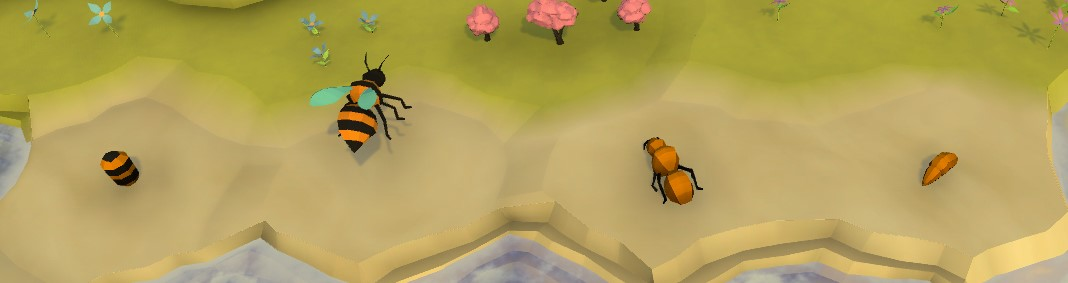
\includegraphics[width=300px]{0.bilder/metamorphosisimplemented.jpg}
    \end{center}
    \caption{Vier verschiedene Stadien des Bienenmodells von links nach rechts: Ei, Adult, Puppe und Larve} \label{image:metamorphosisimplemented}
\end{figure}

\subsubsection{Brutvorgang}
Um neue Bienen herzustellen werden, wie bereits zuvor erläutert und in \autoref{image:reproductionloop} erkennbar, verschiedene Bienen für verschiedene Resultate benötigt. Wird ein Ei in eine Brutkammer gelegt, beginnt ab diesem Zeitpunkt die Metamorphose, analog zu den In \textit{Sektion 4.1.4} erläuterten Vorgängen. Das gelegte Ei wird nach einer gegebenen Zeit zu einer Larve, danach zu einer Puppe und anschließend zu einer voll ausgewachsenen Biene. Die Modelle einer einzelnen Einheit sind in \autoref{image:metamorphosisimplemented} zu erkennen.

\paragraph{Stadium 1: Ei} Das Ei liegt nach dem Legen in der Brutwabe. Zu diesem Stadium ist lediglich erkennbar, ob befruchtet oder unbefruchtet. Die Wabe muss ein Mal mit Nahrung, vorzugsweise Nektar oder Honig, gefüllt werden, damit das Ei überlebt. Nach einigen Tagen schlüpft daraus eine Larve und die Nahrung in der Brutwabe ist verbraucht.

\paragraph{Stadium 2: Larve} Die Larve ist das Stadium, in welchem Royal Jelly dazugegeben werden kann. Liegt das Ei in einer Königlichen Brutkammer, wird einmalig Royal Jelly statt gewöhnlicher Nahrung dazugegeben. Damit entwickelt sich eine königliche Puppe statt einer herkömmlichen und die Nahrung wird verbraucht.

\paragraph{Stadium 3: Puppe} Die Puppe benötigt, anders als die anderen Stadien, zusätzlich zur Nahrung noch Bienenwachs, welches die Brutwabe bedeckt. Zuerst muss Nahrung dazugegeben, danach die Wabe bedeckt werden. Sobald die Biene alt genug ist, schlüpft sie aus der Puppe und bricht durch die Wachsschicht. Eine erwachsene Biene ist somit herangereift.

\paragraph{Stadium 4: Ausgewachsen} Das ausgewachsene Stadium ermöglicht sämtliche Aktionen einer Biene. In diesem Stadium befinden sich die meisten Bienen. 

\begin{figure}
    \begin{center}
        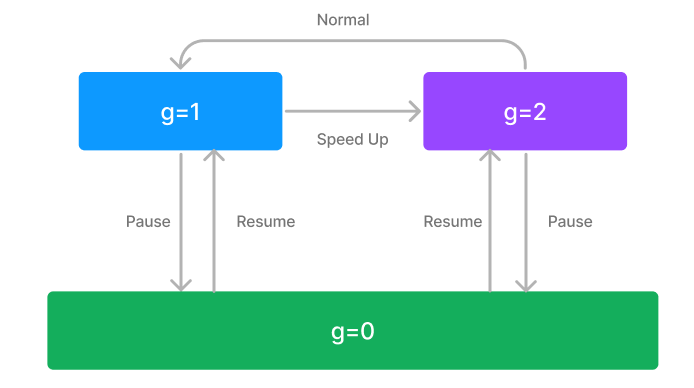
\includegraphics[width=200px]{0.bilder/timecontrol.png}
    \end{center}
    \caption{Zeitsteuerung Zustandsdiagramm} \label{image:timecontrol}
\end{figure}

\subsubsection{Zeitsteuerung}
Analog zu RimWorld wird nach [H21] eine Zeitsteuerung zur besseren Kontrolle eingeführt. Zur Auswahl stehen dabei \textit{Pause} beziehungsweise \textit{Fortführen} (engl. \textit{Resume}) als sich abwechselnde Zustände, und weiterhin \textit{Normal} und \textit{Erhöht}, wobei \textit{Pause} die Geschwindigkeit des Spiels auf $g=0$ setzt, \textit{Normal} die Geschwindigkeit auf $g=1$ setzt, und \textit{Erhöht} die Geschwindigkeit auf $g=2$ setzt. Allerdings wird eine intelligentere Logik verwendet, um das Nutzererlebnis zu erhöhen, welche in \autoref{image:timecontrol} veranschaulicht wird. Pausiert der Nutzer das Spiel, während die Geschwindigkeit auf g=2 steht, wird sich dieser Wert gemerkt, und bei Klick auf den nun vorhandenen Resume-Button wiederhergestellt. Analog funktioniert dieser Prozess auch bei g=1.


\subsection{Interface}
Für alle genannten Mechaniken und Informationen muss ein passendes Interface erstellt werden. Der erste Prototyp ist erkennbar in Form eines Mockups in  \autoref{image:interfaceprototype}. Das Interface wird aus einzelnen Komponenten bestehen, welche in der Grafik durch die rot markierten Bereiche erkennbar sind und in folgenden Paragraphen mit (X) referenziert werden, wobei X dem roten Bereich mit der Zahl X in \autoref{image:interfaceprototype} zugeordnet wird.

\begin{figure}
    \begin{center}
        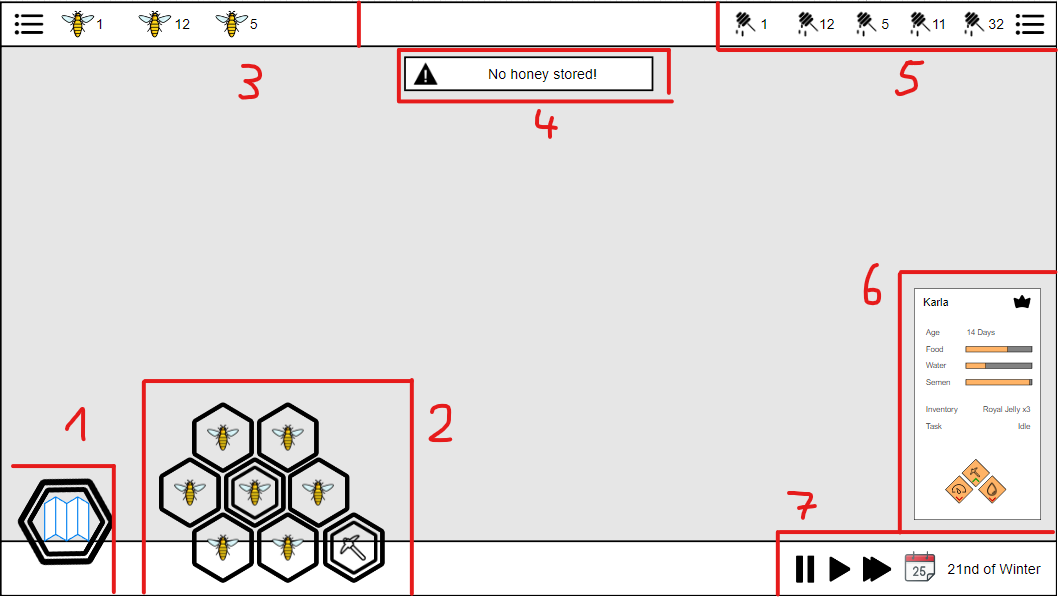
\includegraphics[width=300px]{0.bilder/interfaceprototype.png}
    \end{center}
    \caption{Erster Prototyp des Spielinterfaces} \label{image:interfaceprototype}
\end{figure}

\subsubsection{Karte wechseln}
Um zwischen der Außenwelt und dem inneren des Bienenstocks hin- und herzuwechseln gibt es den Button, welcher in Bereich (1) von \autoref{image:interfaceprototype} dargestellt wird. Befindet sich die Kamera in der Außenwelt, ist auf diesem Knopf ein Bienenstock abgebildet, befindet sich die Kamera im Bienenstock ist dort ein Baum abgebildet, welcher Symbolisch für die Außenwelt steht.

\subsubsection{Action Buttons}
Zur Steuerung der Bienen bedarf es verschiedener auswählbaren Aktionen, welche bereits zuvor erläutert wurden. Es gibt insgesamt 12 verschiedene Aktionen, welche in zwei hexagonale Menüs aufgeteilt sind, zum einen die Tätigkeiten und zum anderen die Strukturen. Diese Menu Buttons sind mit einem zweiten, inneren Hexagon markiert und in Bereich (2) auffindbar. Klickt man auf den jeweiligen Menü-Knopf öffnen sich die jeweils 6 untergeordneten Buttons. Ist währenddessen das andere Menü geöffnet, wird es geschlossen. Es kann somit maximal nur ein Menü gleichzeitig aktiv sein, aber es können beide zeitgleich geschlossen werden. Für den in der Arbeit angefertigten Prototypen werden lediglich die Aktionen \textit{Gather}, \textit{Pollinate}, \textit{Build Storage}, \textit{Lay Eggs} und \textit{Cancel} funktional implementiert. Die ursprüngliche Idee war es, sämtliche Aktionen in ein Menü zu verpacken, wurde dann jedoch aufgrund der schlechteren Übersicht verworfen und aufgeteilt.

\subsubsection{Bee List}
Für einen besseren Überblick der Anzahl verschiedener in der Kolonie vorhandener Kasten wird eine kleine Übersicht dargestellt (3). Zum jeztigen Zeitpunkt werden dort 6 verschiedene Werte angezeigt, je ein Element pro Kaste und je ein Element pro prä-adulter Biene je Kaste. Der Button an der linken Seite öffnet die Liste der Prioritäten, welche bereits zuvor erläutert wurde (vgl. \autoref{image:prioritylist}). Die Grafiken der jeweiligen Kaste oder des Jobs sind noch nicht unterschiedlich dargestellt. 

\subsubsection{Alerts}
Damit der Spieler leichter Überblick über kritische Situationen, wie auch stattfindende Events, haben kann, wird in der Mitte des Bildschirms eine kleine Benachrichtigung visualisiert (4). Ein Alert bleibt für einen kurzen Moment und verschwindet dann wieder, der Spieler wird damit angeregt, aufmerksamer zu spielen und bedient sich der Hypothese [H8]. In dem Prototyp kann mit Drücken der Taste 9 auf der Tastatur für Testzwecke ein kleiner Alert aufgerufen werden. In der späteren Implementierung können sehr einfach neue Alerts ergänzt werden.

\subsubsection{Resource List}
Analog zu RimWorld wird dem Spieler der globale Speicherzustand aller Ressourcen angezeigt (5). Es werden also die Summen aller verschiedenen sammel- und tragbaren Ressourcen angezeigt: \textit{Nectar, Pollen, Wax, Honey} und \textit{Royal Jelly}. Der Button auf der rechten Seite ist im Prototypen noch nicht funktional, soll aber eine Statistik offenbaren, um den Verlauf der Ressourcenstände zu visualisieren. Dies soll dem Spieler etwas mehr Überblick über den Werteverlauf der Kolonie bieten. Da das Lager noch nicht funktional, sondern lediglich dekorativ ist, wird jederzeit bei jeder Ressource eine 0 angezeigt.

\subsubsection{Infofenster}
An der rechten Seite des Bildschirms ist ein Infofenster auffindbar, welches Informationen zum ausgewählten Objekt darstellt. In dem Mockup des Prototypen ist das angezeigte Infofenster jenes, welches bei Auswahl einer Biene gezeigt wird (6). Es werden unter anderem Hunger, Durst, Traits und momentane Aufgabe dargestellt.

\subsubsection{Time Control}
Ebenfalls analog zu RimWorld ist eine Zeitsteuerung implementiert, welche bereits zuvor erläutert wurde. Auf der rechten Seite dieser Steuerung wird das derzeitige Datum angezeigt in dem Format \textit{Year A, Day B of C, Dh}, wobei A das derzeitige Jahr, B der momentane Tag, C die derzeitige Jahreszeit und D die momentane Stunde ist (7). Wie bereits zuvor aufgezeigt gibt es drei verschiedene Grade der Zeit, g=0, g=1 und g=2.

\subsubsection{Start Screen}
Das Interface, welches dem Spieler als allererstes gezeigt wird, ist der Start Screen, welcher für den Anfang sehr simpel gehalten ist nach Hypothese [H1]. Es werden lediglich zwei Buttons zum Erstellen und Laden eines Spielstands angezeigt, ein Hintergrund des Spiels und eine Überschrift mit dem Titel des Spiels \autoref{image:startscreen}. Das Laden und Speichern eines Spielstands sind im Prototyp noch nicht implementiert, die Fundamente dafür sind jedoch bereitgestellt.

\begin{figure}
    \begin{center}
        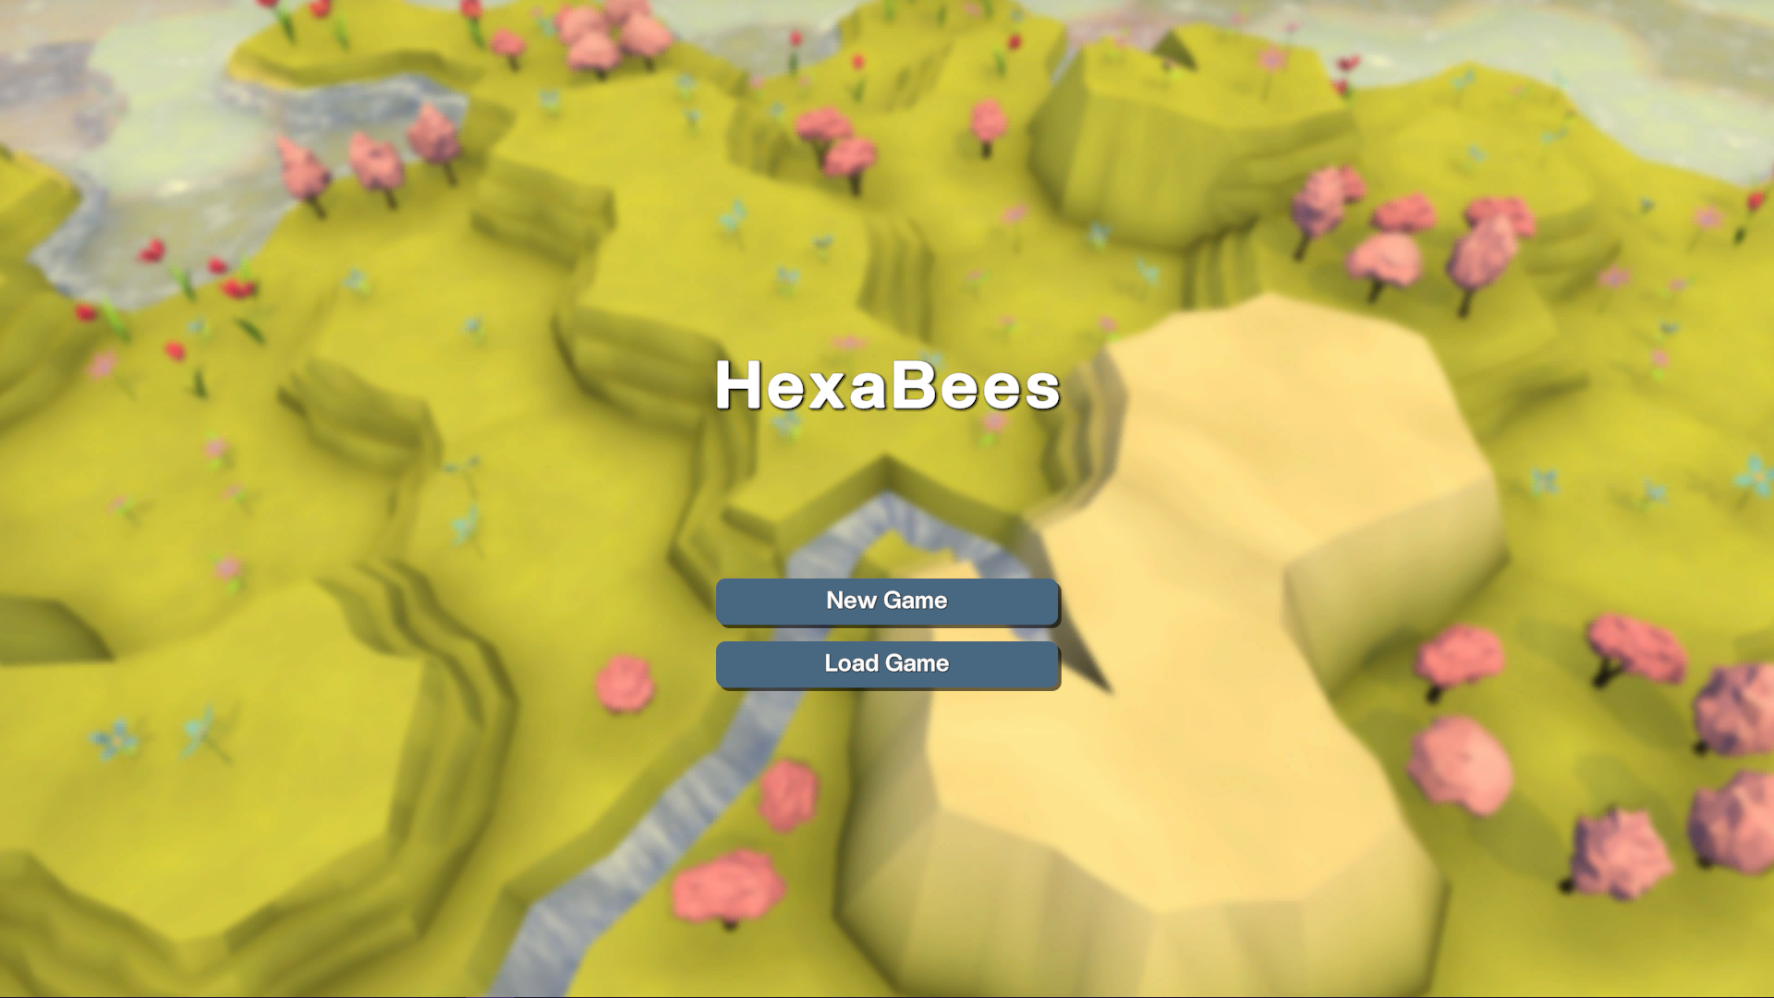
\includegraphics[width=300px]{0.bilder/startscreen.png}
    \end{center}
    \caption{Start Screen des Spiels} \label{image:startscreen}
\end{figure}

\subsubsection{Spielwelt}
Der hellgraue Bereich in \autoref{image:interfaceprototype} stellt die interaktive Spielwelt dar, in welcher die Aktionen angegeben werden können und die Einheiten sich dementsprechend verhalten.
\subsection{User Testing}
Für den Abschluss der Implementierung des Prototypen wird ein letzter Test durchgeführt in Form eines User Testing beziehungsweise Produkttests. Der zuvor entwickelte Prototyp mit dem Arbeitstitel \textit{HexaBees} wird in einer letzten Iteration von einem ausgewählten Probanden getestet, wobei sich jegliche Eindrücke, Ideen und Probleme bei der Auseinandersetzung notiert werden, um in späteren Implementationszyklen eingebunden zu werden. Da der zuvor erarbeite Gameplay Loop nicht vollständig im Prototyp vorhanden ist, wird der Gameplay Loop lediglich theoretisch erörtert und das Feedback dazu notiert. Selbstverständlich wäre es interessant, die Eindrücke und Ideen von mehreren Personen aufzugreifen, das Testing wird der Einfachheit halber und aus zeitlichen Gründen allerdings nicht auf mehrere Personen erweitert.

\subsubsection{Versuchsaufbau}
Analog zu den Interviews stehen im Produkttest erneut die Fragen und Beobachtung im Vordergrund. Jedoch ist nun die Versuchszeit auf 15 Minuten heruntergesetzt, da sich der Prototyp in einem recht frühen Stadium befindet. Das Transkript zu dem Produkttest befindet sich erneut im Anhang als \hyperref[transcript:D]{Transkript D}. Anders als im Interview wird der Produkttest auf eine einzelne Phase begrenzt, den \textit{Hauptteil}. In diesem werden Fragen zu sowohl Interface Design, als auch Gameplay Loop oder Spaßfaktor gestellt.

\paragraph{Hauptteil}
\begin{itemize}
    \item F1: Wie findest du das Farbschema?
    \item F2: Ist das User Interface übersichtlich?
    \item F3: Findest du die Grafiken ersichtlich und hilfreich?
    \item F4: Ist die Zeit gut erkennbar?
    \item F5: Ist der Sinn der Zeitsteuerung klar?
    \item F6: Wie findest du die generierte Welt?
    \item F7: Findest du es sinnvoll, dass Bienenstock und Außenwelt getrennt sind?
    \item F8: Wie findest du die Auswahl der Ressourcen?
    \item F9: Was hältst du von dem Gameplay Loop?
    \item F10: Denkst du, das voll implementierte Spiel hätte einen gewissen Faktor an Spaß und eine Langzeitmotivation?
\end{itemize}

\subsubsection{Proband}
Der ausgewählte Proband war bereits im zuvor durchgeführten Interview als Proband aufgetreten und hat daher mit absoluter Sicherheit Kontakt mit Resource Management Games gehabt. Da mit den Hypothesen der Prototyp erarbeitet wurde, und damit ein großer Fokus auf Einsteigerfreundlichkeit gelegt wurde, empfiehlt es sich, auf Proband A zurückzugreifen, welcher tendenziell weniger Erfahrung mit Videospielen im Allgemeinen vorweist, als die anderen beiden Probanden.

\subsubsection{Ablauf}
Der Produkttest beginnt, wie bereits zuvor erläutert, direkt mit dem Einblick in das Spielgeschehen. Im Folgenden werden Ergebnisse beziehungsweise Konklusionen mit [KX] gekennzeichnet, welche sich in \autoref{table:conclusions} aufgelistet wiederfinden, wobei das X für die Kennziffer der jeweiligen Konklusion steht. Es wird auf einzelne Hypothesen aus \autoref{table:hypotheses} zurückgegriffen, welche mit gegebenen Konklusionen unterstützt werden und wie bereits zuvor mit [HX] referenziert werden.

Es zeigt sich, dass das Menü noch sehr übersichtlich gehalten ist, wodurch auch ein unerfahrener Proband direkt spielen kann. Zwei Buttons zum Erstellen und Laden eines Spielstandes sind für die nahe Zukunft ausreichend, wodurch sich [H1] bestätigt [K1][Z.4-5]. Die Kamerasteuerung ist scheinbar sehr intuitiv und fühlt sich auch für Menschen mit weniger Erfahrung gut an, weder zu schnell, noch zu langsam, wodurch [H16] gestützt wird. [K2][Z.7-8, Z.69]. Die Farbpalette des UI ist angenehm und passt zum Spiel [K3][Z.13-14]. Auch die Hexagone sind intuitiv gesehen passend für das Spiel hinsichtlich der Thematik [K4][Z.15-18]. Das User-Interface ist selbsterklärend und übersichtlich, auch Menschen mit sehr wenig Erfahrung sind in der Lage, zu erkennen, welche Informationen wo dargestellt werden [K5][Z.19-29].  Die Grafiken im UI scheinen die Überforderung eines Neuanfängers deutlich zu senken und erhöhen das Spielgefühl, wodurch [H14] und [H18] gestützt werden. Die Ausnahme hierbei macht der Nektar, welcher gegebenenfalls mit Honig verwechselt werden kann [Z.46-49]. Diese Fehlinterpretation könnte aber mit einem einfachen Tutorial sehr schnell vermieden werden, wie bereits mit [H20] erörtert. Die Zeit ist gut erkenntlich dargestellt und belegt einen eigenen Quadranten im Bildschirm, ohne beidseitig von weiteren Elementen und Informationen umgeben zu sein, womit [H10] erfolgreich umgesetzt wurde [K6]. Die Zeitsteuerung ergibt im Kontext des Gameplay Loops ergibt auch ohne Videospiel-Erfahrung Sinn und stützt damit [H21][K7][Z.32-35]. Die Trennung der beiden Karten (Außenwelt, Bienenstock) ist ersichtlich, aber eine komplette Trennung wäre nicht sinnvoll [K8][Z.36-44]. Da dies ohnehin nicht geplant war, müssen keine Ideen verworfen werden. Das Gegenteil jedoch ist der Fall, da Proband D die eigentlich geplante Idee selber aufwirft und damit unterstützt [Z.37-41]. Die Anzahl und Variation der Ressourcen scheint ausreichend und intuitiv zu sein in Kontext von einer Bienenkolonie [K9][Z.45-53]. Im Produkttest wurde festgestellt, dass ein Icon falsch implementiert wurde (Honig statt Royal Jelly), was jedoch im Nachhinein behoben wurde [Z.51]. Der Gameplay Loop klingt für Proband D interessant, wenn auch sehr heruntergebrochen auf die wichtigsten Aspekte des Spiels [K10][Z.54-58]. Proband D bringt die Anregung auf, mehr Details in das Spiel einzubauen, beispielsweise Fressfeinde der Bienen, etwa Bären [Z.60-62]. Diese Idee könnte als Hypothese für eine zukünftige Iteration aufgenommen werden, wird für diese Arbeit jedoch nicht weiter untersucht. Außerdem sollten die Bäume von Modell her nicht der gleichen Größe wie die Blumen entsprechen [Z.62]. Diese Anpassung wird aufgrund zeitlicher Umstände vorerst nicht durchgeführt, aber in naher Zukunft umgesetzt. Ein gewisser Spaßfaktor und eine Langzeitmotivation, gegebenenfalls durch replayability, sind ersichtlich und könnten bei Fertigstellung durchaus vorhanden sein, selbst wenn der Proband selber nicht viel Kontakt mit Videospielen hat [K11][Z.63-67].

\begin{table}[]
    \centering
    \caption{Übersicht aller aufgestellten Konklusionen des Produkttests}
    \label{table:conclusions}
    \begin{tabular}{|l|l|}
    \hline
    K1 & Zwei Buttons im Startmenü sind vorerst ausreichend    \\ \hline
    K2 & Die Kamerasteuerung ist optimal                       \\ \hline
    K3 & Die gewählte Farbpalette ist angenehm                 \\ \hline
    K4 & Hexagone unterstreichen die Thematik und sind passend \\ \hline
    K5 & Das User-Interface ist übersichtlich                  \\ \hline
    K6 & Die Zeit ist gut erkennbar dargestellt                 \\ \hline
    K7 & Eine Zeitsteuerung ist eine gute Ergänzung                  \\ \hline
    K8 & Die Trennung zwischen Außenwelt und Bienenstock ist gut                  \\ \hline
    K9 & Die Anzahl und Auswahl der Ressourcen ist zufriedenstellend                  \\ \hline
    K10 & Der Kern des Gameplay Loops ist interessant                  \\ \hline
    K11 & Ein Spaßfaktor und eine Langzeitmotivation sind erkennbar                  \\ \hline
    \end{tabular}
\end{table}
\subsection{Abschluss}
Um die Implementierung des Prototypen abzuschließen werden die erarbeiteten Hypothesen angeschaut und erörtert, inwiefern diese umgesetzt werden konnten. Als Fundament der wissenschaftlich erarbeiteten Grundlage der Konzeption des Spiels ist dieser Schritt unerlässlich und 

\paragraph*{H1}
Das Startmenü im Prototypen besitzt lediglich zwei Buttons zum Erstellen und Laden eines Spielstandes. Der Button zum Laden ist momentan noch nicht funktionsfähig, wird in naher Zukunft aber implementiert. 

\paragraph*{H2}
Die Steuerung oberhalb der Karte anzuzeigen ist scheinbar nicht weiter nötig wie der Produkttest gezeigt hat. Sollte die Steuerung komplexer werden, könnte diese Hypothese erneut aufgegriffen werden.

\paragraph*{H3}
Für den Moment sind noch keine optionalen Inhalte implementiert, aber sollten optionale Umgebungsinhalte für eine höhere Schwierigkeit eingefügt werden, beispielsweise die im Produkttest aufgezeigte Idee der Bären als Fressfeinde, sollte dieser Schritt umgesetzt werden.

\paragraph*{H4}
Dieser Aspekt sollte unbedingt im Laufe der Zeit gegeben sein. Je schneller verschiedene Sprachen unterstützt werden, desto einfacher werden zukünftige Iterationen, da weniger nachimplementiert werden muss, und bei jedem neuen Wort oder Begriff die Übersetzung direkt hinzugefügt werden kann statt nachträglich. Dieser Schritt der Inklusion ist essenziell um eine breitere Masse ansprechen zu können und daher auch kommerziell interessant.

\paragraph*{H5}
Der Plan im Gameplay Loop ist es, den Bienenstock zufällig zu platzieren, sodass der Spieler mal bessere und mal schlechtere Startbedingungen hat. Damit ist dieser Schritt zwar momentan noch nicht umgesetzt, aber im Design berücksichtigt.

\paragraph*{H6}
Zur Zeit des Prototypen gibt es 18 theoretisch implementierte Traits, welche in \autoref{table:traits} zu finden sind. Allerdings haben diese noch nicht die richtigen Grafiken zugeordnet und noch keine Effekte auf das Spielgeschehen, werden jedoch bereits zufällig zugeordnet.

\paragraph*{H7}
Da die Traits noch nicht vollends implementiert sind, ist diese Hypothese noch nicht vollends erfüllt. Jedoch ist diese Hypothese im Design vorgemerkt und soll keine direkte Entscheidung über beste oder schlechteste Traits zulassen.

\paragraph*{H8}
Diese Hypothese ist mit dem Konzept des Alerts umgesetzt wurde, wenn auch nicht in Fülle angewandt.

\paragraph*{H9}
Durch das Konzept der Storage als baubare, kachel-belegende Struktur mittels Aktionen und Anweisungen ist diese Hypothese umgesetzt worden.

\paragraph*{H10}
Das User Testing hat gezeigt, dass die gewählte Stelle der Uhrzeit und des Datums gut erkennbar sind.

\paragraph*{H11}
Diese Idee könnte nach wie vor umgesetzt werden, würde die Komplexität jedoch stark erhöhen. Eine mögliche Umsetzung der Temperatur könnte eine Jahreszeitenbedingte Außentemperatur mit sich bringen, und eine Mindestanzahl benötigter Bienen im Bienenstock, um die Temperatur hoch genug für das Überleben zu halten. Dieses System wird in naher Zukunft jedoch voraussichtlich nicht implementiert.

\paragraph*{H12}
Diese Hypothese wurde versucht im Design zu berücksichtigen, sodass sowohl die Ressourcen, als auch die Converter und die Schritte der Ressourcenumwandlung intuitiv sind.

\paragraph*{H13}
Das in RimWorld gezeigte Prioritätensystem wurde funktionsfähig implementiert und stellt einen festen Kernbestandteil des Spiels dar.

\paragraph*{H14}
Die verschiedenen Stufen der jeweiligen Prioritäten wurden grafisch umgesetzt, womit die Hypothese in das Spielgeschehen übernommen wurde.

\paragraph*{H15}
Das indirekte Anweisen ist implementiert worden mittels der im Quellcode ersichtlichen JobQueue und der JobOrder. 

\paragraph*{H16}
Die Steuerung scheint, laut User Testing, sehr intuitiv zu sein, wodurch diese Hypothese unmittelbar in das Spiel integriert wurde.

\paragraph*{H17}
Durch die zufällig generierte Karte, und den im Design vorgemerkten zufälligen Startpunkt des Bienenstocks, wie auch den verschiedenen Traits, ist einiges an Zufall im Spiel enthalten. Dadurch wird versucht, diese Hypothese weiter zu integrieren und damit die replayability zu steigern.

\paragraph*{H18}
Dieser Aspekt wurde stark berücksichtigt, wodurch in jedem Quadranten des User-Interface mehrere Icons zu finden sind, wie auch in der Prioritätenliste. Es zeigt sich, dass eventuell Fehlinterpretationen auftreten können, welche jedoch mit einem Tutorial sehr leicht beseitigt werden können.

\paragraph*{H19}
Diese Hypothese konnte durch den kleinen Umfang des Prototypen nicht in das Spiel integriert werden, ist im Design jedoch vorgemerkt.

\paragraph*{H20}
Auch diese Hypothese konnte aufgrund der kurzen Zeitspanne noch nicht in das Spiel integriert werden, ist jedoch unerlässlich und steht neben der Integration verschiedener Sprachen weit oben auf der Liste der zukünftigen Iterationen.

\paragraph*{H21}
Das User-Testing hat gezeigt, dass die Zeitsteuerung ein durchaus gut verstandenes Konzept darstellt und die Kontrolle des Nutzers verstärkt. Es ergeben sich daraus keinerlei Nachteile für den Spieler und ist damit ein bleibendes Element des Spiels.
\subsection{Unit Tests}
Um die Stabilität der Anwendung im Allgemeinen zu gewährleisten, und die Zuverlässigkeit der einzelnen Funktionen sicherzustellen, werden, auch im Bereich des Game Development, sogenannte \textit{Unit Tests} verwendet. Es gibt dabei mehrere Vorteile dieser Tests. Man kann beispielsweise mit diesen Tests Szenarien abdecken, welche nur sehr selten im produktiven Anwendungsfall auftreten würden, sogenannte \textit{Corner Cases}. Außerdem ist die Chance deutlich geringer, dass bereits aufgetretene Bugs, welche durch Unit Tests bereits behoben wurden, erneut auftreten. Der größte Nachteil dieser Tests ist der Fakt, dass deutlich mehr Code geschrieben werden muss, was sehr viel Zeit einfordert \cite*[]{unittests}. In einem industriellen Umfeld und bei der Entwicklung einer marktreifen Anwendung ist dieser Schritt allerdings unerlässlich. Es ist daher sinnvoll, auch im weiteren Verlauf, Unit Tests für die gesamte Anwendung nachträglich hinzuzufügen. Aufgrund der kurzen Zeitspanne und dem bereits großen Umfang des Quellcodes wird in dieser Arbeit bewusst auf diese Art des Testings verzichtet.
\subsection{Ausblick}
Das Projekt wird in Zukunft fortgesetzt. Der Grundstein wurde gelegt und scheint, laut Ergebnissen, auch vielversprechend zu sein. Neben den bereits konzipierten Mechaniken und Elementen, welche mit Sicherheit implementiert werden, gibt es weitere Ideen, die erörtert werden müssen. Eine solche Idee wäre der Mensch als natürlicher Feind der Bienen. Es könnten zu Beginn des Spiels einige Kacheln, je nach Größe der Gesamtkarte, mit kleinen Dörfern belegt sein. Über die Zeit breiten sich diese Dörfer dann aus auf vorzugsweise zufällige Nachbarkacheln aus. Ist eine Kachel mit einem Dorf vollständig umringt von Kacheln mit Dörfern, wird aus dem Dorf eine Stadt. Dörfer und Städte beherbergen Menschen, welche das Klima beeinflussen, wodurch mit der Zeit die Temperatur (falls implementiert), wie auch der Meeresspiegel, die Flüsse und die Vegetation verändert wird. Außerdem belegen die Dörfer mehr und mehr Kacheln, welche Blumen zerstören und das Erstellen neuer Blumen unmöglich machen. 

\section{Fazit}
Es wurde binnen 8 Wochen ein Prototyp auf Grundlage von wissenschaftlicher Arbeit und kreativem Input konzipiert, implementiert und getestet. Es hat sich gezeigt, dass die ausgewählte Thematik der Bienenkolonie einen äußerst vielversprechender Kontext für kreative und mechanisch interessante Ideen darstellt, welche viel Potenzial für künftige Iterationen bieten. Einer der wohl wichtigsten Erkenntnisse ist, dass das Einbinden von Probanden mittels Interviews und User Testing in die Konzipierung des Spiels sehr große Vorteile mit sich bringt. Es zeigt sich damit, dass Methoden der nutzungsorientierten Gestaltung positive Einflüsse auf den Verlauf der Entwicklung eines Videospiels haben. Außerdem war es in Retrospektive die richtige Entscheidung, Probanden mit jeweils drei verschiedenen Erfahrungsgraden zu wählen, da die daraus gewonnen Ergebnisse sehr hilfreich für die Konzipierung des Spiels waren. Es existiert großes Potenzial für die Weiterentwicklung, wodurch dieses Projekt mit enormer Sicherheit weitergeführt wird. Es ist zum Stand der Arbeit noch nicht ersichtlich, wie viele Iterationen noch benötigt werden, um das Projekt abzuschließen. Allerdings waren es erfreulicherweise wenige Bugs, die im Laufe der Implementierung behoben werden mussten, was den Entwicklungsprozess deutlich vereinfacht hat. Es wurde ein Großteil der Hypothesen umgesetzt, wenn nicht praktisch dann trotzdem theoretisch im Konzept, was als Erfolg angesehen werden kann. Es besteht ein Gameplay Loop, ein Spielbeginn, ein Spielende und viele durchaus interessante Mechaniken, die das Spiel von anderen Titeln des Genres abheben, gleichzeitig aber auch auf gut funktionierende Elemente anderer Vertreter fundieren. Alles in allem ist die Arbeit, und damit auch das Projekt, ein voller Erfolg. Der Prototyp ist sowohl als bereits gebaute Version, wie auch als Unity Projekt auf dem Datenträger enthalten.

\newpage
\printbibliography

\newpage
\section*{Notizen}
\subsection*{Offene Fragen}
\begin{itemize}
    \item Age of Empires und Civ noch ausbauen?
    \item Genauer auf alle Nachfolger und Vorgänger eingehen, mit Publishern, Developern und Änderungen?
    \item Wirklich alle verfügbaren Rezensionen suchen und reinpacken?
    \item Umfrage zu gespielten Klassikern über Discord?
    \item Noch Anno 1602 als Klassiker hinzufügen?
    \item Notable Mentions? Cruisader Kings, Anno 1602, 
\end{itemize}

\subsection*{Ideen}
\begin{itemize}
    \item HexaBees turn based, oder RTS?
    \item Falls RTS dann 
\end{itemize}

\subsection*{Fremdwörter}
\begin{itemize}
    \item Game engine
    \item Real Time Strategy
    \item launch arcos
    \item Singeplayer (Game)
    \item Isometrisch
    \item Domination
    \item Space Race
    \item 
\end{itemize}

\subsection*{Abkürzungen}
\begin{itemize}
    \item SAT - Sega Saturn, Konsole
    \item RTS
    \item R - Residents
    \item C - Commercial
    \item I - Industries
    \item KI
    \item 
\end{itemize}
\end{document}